\documentclass[twoside,openright,titlepage,numbers=noenddot,headinclude,%
               footinclude=true,cleardoublepage=empty,abstractoff,BCOR=5mm,%
               paper=a4,fontsize=12pt,ngerman,american]{scrreprt}

% Solve too many packages
\usepackage{etex}
\reserveinserts{28}

% Custom config ===============================================================

% Classic thesis
\usepackage{amssymb}
% ****************************************************************************************************
% classicthesis-config.tex
% formerly known as loadpackages.sty, classicthesis-ldpkg.sty, and classicthesis-preamble.sty
% Use it at the beginning of your ClassicThesis.tex, or as a LaTeX Preamble
% in your ClassicThesis.{tex,lyx} with % ****************************************************************************************************
% classicthesis-config.tex
% formerly known as loadpackages.sty, classicthesis-ldpkg.sty, and classicthesis-preamble.sty
% Use it at the beginning of your ClassicThesis.tex, or as a LaTeX Preamble
% in your ClassicThesis.{tex,lyx} with % ****************************************************************************************************
% classicthesis-config.tex
% formerly known as loadpackages.sty, classicthesis-ldpkg.sty, and classicthesis-preamble.sty
% Use it at the beginning of your ClassicThesis.tex, or as a LaTeX Preamble
% in your ClassicThesis.{tex,lyx} with \input{classicthesis-config}
% ****************************************************************************************************
% If you like the classicthesis, then I would appreciate a postcard.
% My address can be found in the file ClassicThesis.pdf. A collection
% of the postcards I received so far is available online at
% http://postcards.miede.de
% ****************************************************************************************************

% ****************************************************************************************************
% 1. Configure classicthesis for your needs here, e.g., remove "drafting" below
% in order to deactivate the time-stamp on the pages
% ****************************************************************************************************
\PassOptionsToPackage{eulerchapternumbers,listings,drafting,
				 pdfspacing,eulermath,%floatperchapter,%linedheaders,%
				 subfig,parts,dottedtoc}{classicthesis}
% ********************************************************************
% Available options for classicthesis.sty
% (see ClassicThesis.pdf for more information):
% drafting
% parts nochapters linedheaders
% eulerchapternumbers beramono eulermath pdfspacing minionprospacing
% tocaligned dottedtoc manychapters
% listings floatperchapter subfig
% ********************************************************************

% ********************************************************************
% Triggers for this config
% ********************************************************************
\usepackage{ifthen}
\newboolean{enable-backrefs} % enable backrefs in the bibliography
\setboolean{enable-backrefs}{true} % true false
% ****************************************************************************************************


% ****************************************************************************************************
% 2. Personal data and user ad-hoc commands
% ****************************************************************************************************
\newcommand{\myTitle}{Example-Dependent Cost-Sensitive Classification\xspace}
\newcommand{\mySubtitle}{Applications in Financial Risk Modeling and Marketing Analytics\xspace}
\newcommand{\myDegree}{Doktor-Ingenieur (Dr.-Ing.)\xspace}
\newcommand{\myName}{Alejandro Correa Bahnsen\xspace}
\newcommand{\myProf}{Put name here\xspace}
\newcommand{\myOtherProf}{Put name here\xspace}
\newcommand{\mySupervisor}{Bj\"orn~Ottersten\xspace}
\newcommand{\myFaculty}{Doctoral School of Computer Science and Computer Engineering\xspace}
\newcommand{\myDepartment}{Department of EE and CS\xspace}
\newcommand{\myUni}{University of Luxembourg\xspace}
\newcommand{\myLocation}{Luxembourg, Luxembourg\xspace}
\newcommand{\myTime}{July 2015\xspace}
\newcommand{\myVersion}{version 0.7\xspace}


% ********************************************************************
% Setup, finetuning, and useful commands
% ********************************************************************
\newcounter{dummy} % necessary for correct hyperlinks (to index, bib, etc.)
\newlength{\abcd} % for ab..z string length calculation
\providecommand{\mLyX}{L\kern-.1667em\lower.25em\hbox{Y}\kern-.125emX\@}
\newcommand{\ie}{i.\,e.}
\newcommand{\Ie}{I.\,e.}
\newcommand{\eg}{e.\,g.}
\newcommand{\Eg}{E.\,g.}
% ****************************************************************************************************


% ****************************************************************************************************
% 3. Loading some handy packages
% ****************************************************************************************************
% ********************************************************************
% Packages with options that might require adjustments
% ********************************************************************
% \PassOptionsToPackage{latin9}{inputenc}	% latin9 (ISO-8859-9) = latin1+"Euro sign"
%  \usepackage{inputenc}

%\PassOptionsToPackage{ngerman,american}{babel}   % change this to your language(s)
% Spanish languages need extra options in order to work with this template
%\PassOptionsToPackage{spanish,es-lcroman}{babel}
 \usepackage{babel}

\PassOptionsToPackage{square,authoryear}{natbib}
 \usepackage{natbib}

\PassOptionsToPackage{fleqn}{amsmath}		% math environments and more by the AMS
 \usepackage{amsmath}

% ********************************************************************
% General useful packages
% ********************************************************************
\PassOptionsToPackage{T1}{fontenc} % T2A for cyrillics
	\usepackage{fontenc}
\usepackage{lipsum}
\usepackage{textcomp} % fix warning with missing font shapes
%\usepackage{scrhack} % fix warnings when using KOMA with listings package
\usepackage{xspace} % to get the spacing after macros right
\usepackage{mparhack} % get marginpar right
\usepackage{fixltx2e} % fixes some LaTeX stuff
\PassOptionsToPackage{printonlyused,smaller}{acronym}
	\usepackage{acronym} % nice macros for handling all acronyms in the thesis
%\renewcommand*{\acsfont}[1]{\textssc{#1}} % for MinionPro
%\renewcommand{\bflabel}[1]{{#1}\hfill} % fix the list of acronyms
% ****************************************************************************************************


% ****************************************************************************************************
% 4. Setup floats: tables, (sub)figures, and captions
% ****************************************************************************************************
\usepackage{tabularx} % better tables
	\setlength{\extrarowheight}{3pt} % increase table row height
\newcommand{\tableheadline}[1]{\multicolumn{1}{c}{\spacedlowsmallcaps{#1}}}
\newcommand{\myfloatalign}{\centering} % to be used with each float for alignment
\usepackage{caption}
\captionsetup{format=hang,font=small}
\usepackage{subfig}
% ****************************************************************************************************


% ****************************************************************************************************
% 5. Setup code listings
% ****************************************************************************************************
\usepackage{listings}
%\lstset{emph={trueIndex,root},emphstyle=\color{BlueViolet}}%\underbar} % for special keywords
\lstset{language=[LaTeX]Tex,%C++,
    keywordstyle=\color{RoyalBlue},%\bfseries,
    basicstyle=\small\ttfamily,
    %identifierstyle=\color{NavyBlue},
    commentstyle=\color{Green}\ttfamily,
    stringstyle=\rmfamily,
    numbers=none,%left,%
    numberstyle=\scriptsize,%\tiny
    stepnumber=5,
    numbersep=8pt,
    showstringspaces=false,
    breaklines=true,
    frameround=ftff,
    frame=single,
    belowcaptionskip=.75\baselineskip
    %frame=L
}
% ****************************************************************************************************


% ****************************************************************************************************
% 6. PDFLaTeX, hyperreferences and citation backreferences
% ****************************************************************************************************
% ********************************************************************
% Using PDFLaTeX
% ********************************************************************
\PassOptionsToPackage{pdftex,hyperfootnotes=true,pdfpagelabels}{hyperref}
	\usepackage{hyperref}  % backref linktocpage pagebackref
\pdfcompresslevel=9
\pdfadjustspacing=1
\PassOptionsToPackage{pdftex}{graphicx}
	\usepackage{graphicx}

% ********************************************************************
% Setup the style of the backrefs from the bibliography
% (translate the options to any language you use)
% ********************************************************************
\newcommand{\backrefnotcitedstring}{\relax}%(Not cited.)
\newcommand{\backrefcitedsinglestring}[1]{(Cited on page~#1.)}
\newcommand{\backrefcitedmultistring}[1]{(Cited on pages~#1.)}
\ifthenelse{\boolean{enable-backrefs}}%
{%
		\PassOptionsToPackage{hyperpageref}{backref}
		\usepackage{backref} % to be loaded after hyperref package
		   \renewcommand{\backreftwosep}{ and~} % separate 2 pages
		   \renewcommand{\backreflastsep}{, and~} % separate last of longer list
		   \renewcommand*{\backref}[1]{}  % disable standard
		   \renewcommand*{\backrefalt}[4]{% detailed backref
		      \ifcase #1 %
		         \backrefnotcitedstring%
		      \or%
		         \backrefcitedsinglestring{#2}%
		      \else%
		         \backrefcitedmultistring{#2}%
		      \fi}%
}{\relax}

% ********************************************************************
% Hyperreferences
% ********************************************************************
\hypersetup{%
    %draft,	% = no hyperlinking at all (useful in b/w printouts)
    colorlinks=true, linktocpage=true, pdfstartpage=3, pdfstartview=FitV,%
    % uncomment the following line if you want to have black links (e.g., for printing)
    %colorlinks=false, linktocpage=false, pdfborder={0 0 0}, pdfstartpage=3, pdfstartview=FitV,%
    breaklinks=true, pdfpagemode=UseNone, pageanchor=true, pdfpagemode=UseOutlines,%
    plainpages=false, bookmarksnumbered, bookmarksopen=true, bookmarksopenlevel=1,%
    hypertexnames=true, pdfhighlight=/O,%nesting=true,%frenchlinks,%
    urlcolor=webbrown, linkcolor=MidnightBlue, citecolor=MidnightBlue, %pagecolor=RoyalBlue,%
    %urlcolor=Black, linkcolor=Black, citecolor=Black, %pagecolor=Black,%
    pdftitle={\myTitle},%
    pdfauthor={\textcopyright\ \myName, \myUni, \myFaculty},%
    pdfsubject={},%
    pdfkeywords={},%
    pdfcreator={pdfLaTeX},%
    pdfproducer={LaTeX with hyperref and classicthesis}%
}

% ********************************************************************
% Setup autoreferences
% ********************************************************************
% There are some issues regarding autorefnames
% http://www.ureader.de/msg/136221647.aspx
% http://www.tex.ac.uk/cgi-bin/texfaq2html?label=latexwords
% you have to redefine the makros for the
% language you use, e.g., american, ngerman
% (as chosen when loading babel/AtBeginDocument)
% ********************************************************************
\makeatletter
\@ifpackageloaded{babel}%
    {%
       \addto\extrasamerican{%
					\renewcommand*{\figureautorefname}{Figure}%
					\renewcommand*{\tableautorefname}{Table}%
					\renewcommand*{\partautorefname}{Part}%
					\renewcommand*{\chapterautorefname}{Chapter}%
					\renewcommand*{\sectionautorefname}{Section}%
					\renewcommand*{\subsectionautorefname}{Section}%
					\renewcommand*{\subsubsectionautorefname}{Section}%
				}%
       \addto\extrasngerman{%
					\renewcommand*{\paragraphautorefname}{Absatz}%
					\renewcommand*{\subparagraphautorefname}{Unterabsatz}%
					\renewcommand*{\footnoteautorefname}{Fu\"snote}%
					\renewcommand*{\FancyVerbLineautorefname}{Zeile}%
					\renewcommand*{\theoremautorefname}{Theorem}%
					\renewcommand*{\appendixautorefname}{Anhang}%
					\renewcommand*{\equationautorefname}{Gleichung}%
					\renewcommand*{\itemautorefname}{Punkt}%
				}%
			% Fix to getting autorefs for subfigures right (thanks to Belinda Vogt for changing the definition)
			\providecommand{\subfigureautorefname}{\figureautorefname}%
    }{\relax}
\makeatother


% ****************************************************************************************************
% 7. Last calls before the bar closes
% ****************************************************************************************************
% ********************************************************************
% Development Stuff
% ********************************************************************
\listfiles
%\PassOptionsToPackage{l2tabu,orthodox,abort}{nag}
%	\usepackage{nag}
%\PassOptionsToPackage{warning, all}{onlyamsmath}
%	\usepackage{onlyamsmath}

% ********************************************************************
% Last, but not least...
% ********************************************************************
\usepackage{classicthesis}
% ****************************************************************************************************


% ****************************************************************************************************
% 8. Further adjustments (experimental)
% ****************************************************************************************************
% ********************************************************************
% Changing the text area
% ********************************************************************
%\linespread{1.05} % a bit more for Palatino
%\areaset[current]{312pt}{761pt} % 686 (factor 2.2) + 33 head + 42 head \the\footskip
%\setlength{\marginparwidth}{7em}%
%\setlength{\marginparsep}{2em}%

% ********************************************************************
% Using different fonts
% ********************************************************************
%\usepackage[oldstylenums]{kpfonts} % oldstyle notextcomp
%\usepackage[osf]{libertine}
%\usepackage{hfoldsty} % Computer Modern with osf
%\usepackage[light,condensed,math]{iwona}
%\renewcommand{\sfdefault}{iwona}
%\usepackage{lmodern} % <-- no osf support :-(
% \usepackage[T1]{fontenc}
% \usepackage{textcomp}
%\usepackage[urw-garamond]{mathdesign} <-- no osf support :-(
% ****************************************************************************************************

% ****************************************************************************************************
% If you like the classicthesis, then I would appreciate a postcard.
% My address can be found in the file ClassicThesis.pdf. A collection
% of the postcards I received so far is available online at
% http://postcards.miede.de
% ****************************************************************************************************

% ****************************************************************************************************
% 1. Configure classicthesis for your needs here, e.g., remove "drafting" below
% in order to deactivate the time-stamp on the pages
% ****************************************************************************************************
\PassOptionsToPackage{eulerchapternumbers,listings,drafting,
				 pdfspacing,eulermath,%floatperchapter,%linedheaders,%
				 subfig,parts,dottedtoc}{classicthesis}
% ********************************************************************
% Available options for classicthesis.sty
% (see ClassicThesis.pdf for more information):
% drafting
% parts nochapters linedheaders
% eulerchapternumbers beramono eulermath pdfspacing minionprospacing
% tocaligned dottedtoc manychapters
% listings floatperchapter subfig
% ********************************************************************

% ********************************************************************
% Triggers for this config
% ********************************************************************
\usepackage{ifthen}
\newboolean{enable-backrefs} % enable backrefs in the bibliography
\setboolean{enable-backrefs}{true} % true false
% ****************************************************************************************************


% ****************************************************************************************************
% 2. Personal data and user ad-hoc commands
% ****************************************************************************************************
\newcommand{\myTitle}{Example-Dependent Cost-Sensitive Classification\xspace}
\newcommand{\mySubtitle}{Applications in Financial Risk Modeling and Marketing Analytics\xspace}
\newcommand{\myDegree}{Doktor-Ingenieur (Dr.-Ing.)\xspace}
\newcommand{\myName}{Alejandro Correa Bahnsen\xspace}
\newcommand{\myProf}{Put name here\xspace}
\newcommand{\myOtherProf}{Put name here\xspace}
\newcommand{\mySupervisor}{Bj\"orn~Ottersten\xspace}
\newcommand{\myFaculty}{Doctoral School of Computer Science and Computer Engineering\xspace}
\newcommand{\myDepartment}{Department of EE and CS\xspace}
\newcommand{\myUni}{University of Luxembourg\xspace}
\newcommand{\myLocation}{Luxembourg, Luxembourg\xspace}
\newcommand{\myTime}{July 2015\xspace}
\newcommand{\myVersion}{version 0.7\xspace}


% ********************************************************************
% Setup, finetuning, and useful commands
% ********************************************************************
\newcounter{dummy} % necessary for correct hyperlinks (to index, bib, etc.)
\newlength{\abcd} % for ab..z string length calculation
\providecommand{\mLyX}{L\kern-.1667em\lower.25em\hbox{Y}\kern-.125emX\@}
\newcommand{\ie}{i.\,e.}
\newcommand{\Ie}{I.\,e.}
\newcommand{\eg}{e.\,g.}
\newcommand{\Eg}{E.\,g.}
% ****************************************************************************************************


% ****************************************************************************************************
% 3. Loading some handy packages
% ****************************************************************************************************
% ********************************************************************
% Packages with options that might require adjustments
% ********************************************************************
% \PassOptionsToPackage{latin9}{inputenc}	% latin9 (ISO-8859-9) = latin1+"Euro sign"
%  \usepackage{inputenc}

%\PassOptionsToPackage{ngerman,american}{babel}   % change this to your language(s)
% Spanish languages need extra options in order to work with this template
%\PassOptionsToPackage{spanish,es-lcroman}{babel}
 \usepackage{babel}

\PassOptionsToPackage{square,authoryear}{natbib}
 \usepackage{natbib}

\PassOptionsToPackage{fleqn}{amsmath}		% math environments and more by the AMS
 \usepackage{amsmath}

% ********************************************************************
% General useful packages
% ********************************************************************
\PassOptionsToPackage{T1}{fontenc} % T2A for cyrillics
	\usepackage{fontenc}
\usepackage{lipsum}
\usepackage{textcomp} % fix warning with missing font shapes
%\usepackage{scrhack} % fix warnings when using KOMA with listings package
\usepackage{xspace} % to get the spacing after macros right
\usepackage{mparhack} % get marginpar right
\usepackage{fixltx2e} % fixes some LaTeX stuff
\PassOptionsToPackage{printonlyused,smaller}{acronym}
	\usepackage{acronym} % nice macros for handling all acronyms in the thesis
%\renewcommand*{\acsfont}[1]{\textssc{#1}} % for MinionPro
%\renewcommand{\bflabel}[1]{{#1}\hfill} % fix the list of acronyms
% ****************************************************************************************************


% ****************************************************************************************************
% 4. Setup floats: tables, (sub)figures, and captions
% ****************************************************************************************************
\usepackage{tabularx} % better tables
	\setlength{\extrarowheight}{3pt} % increase table row height
\newcommand{\tableheadline}[1]{\multicolumn{1}{c}{\spacedlowsmallcaps{#1}}}
\newcommand{\myfloatalign}{\centering} % to be used with each float for alignment
\usepackage{caption}
\captionsetup{format=hang,font=small}
\usepackage{subfig}
% ****************************************************************************************************


% ****************************************************************************************************
% 5. Setup code listings
% ****************************************************************************************************
\usepackage{listings}
%\lstset{emph={trueIndex,root},emphstyle=\color{BlueViolet}}%\underbar} % for special keywords
\lstset{language=[LaTeX]Tex,%C++,
    keywordstyle=\color{RoyalBlue},%\bfseries,
    basicstyle=\small\ttfamily,
    %identifierstyle=\color{NavyBlue},
    commentstyle=\color{Green}\ttfamily,
    stringstyle=\rmfamily,
    numbers=none,%left,%
    numberstyle=\scriptsize,%\tiny
    stepnumber=5,
    numbersep=8pt,
    showstringspaces=false,
    breaklines=true,
    frameround=ftff,
    frame=single,
    belowcaptionskip=.75\baselineskip
    %frame=L
}
% ****************************************************************************************************


% ****************************************************************************************************
% 6. PDFLaTeX, hyperreferences and citation backreferences
% ****************************************************************************************************
% ********************************************************************
% Using PDFLaTeX
% ********************************************************************
\PassOptionsToPackage{pdftex,hyperfootnotes=true,pdfpagelabels}{hyperref}
	\usepackage{hyperref}  % backref linktocpage pagebackref
\pdfcompresslevel=9
\pdfadjustspacing=1
\PassOptionsToPackage{pdftex}{graphicx}
	\usepackage{graphicx}

% ********************************************************************
% Setup the style of the backrefs from the bibliography
% (translate the options to any language you use)
% ********************************************************************
\newcommand{\backrefnotcitedstring}{\relax}%(Not cited.)
\newcommand{\backrefcitedsinglestring}[1]{(Cited on page~#1.)}
\newcommand{\backrefcitedmultistring}[1]{(Cited on pages~#1.)}
\ifthenelse{\boolean{enable-backrefs}}%
{%
		\PassOptionsToPackage{hyperpageref}{backref}
		\usepackage{backref} % to be loaded after hyperref package
		   \renewcommand{\backreftwosep}{ and~} % separate 2 pages
		   \renewcommand{\backreflastsep}{, and~} % separate last of longer list
		   \renewcommand*{\backref}[1]{}  % disable standard
		   \renewcommand*{\backrefalt}[4]{% detailed backref
		      \ifcase #1 %
		         \backrefnotcitedstring%
		      \or%
		         \backrefcitedsinglestring{#2}%
		      \else%
		         \backrefcitedmultistring{#2}%
		      \fi}%
}{\relax}

% ********************************************************************
% Hyperreferences
% ********************************************************************
\hypersetup{%
    %draft,	% = no hyperlinking at all (useful in b/w printouts)
    colorlinks=true, linktocpage=true, pdfstartpage=3, pdfstartview=FitV,%
    % uncomment the following line if you want to have black links (e.g., for printing)
    %colorlinks=false, linktocpage=false, pdfborder={0 0 0}, pdfstartpage=3, pdfstartview=FitV,%
    breaklinks=true, pdfpagemode=UseNone, pageanchor=true, pdfpagemode=UseOutlines,%
    plainpages=false, bookmarksnumbered, bookmarksopen=true, bookmarksopenlevel=1,%
    hypertexnames=true, pdfhighlight=/O,%nesting=true,%frenchlinks,%
    urlcolor=webbrown, linkcolor=MidnightBlue, citecolor=MidnightBlue, %pagecolor=RoyalBlue,%
    %urlcolor=Black, linkcolor=Black, citecolor=Black, %pagecolor=Black,%
    pdftitle={\myTitle},%
    pdfauthor={\textcopyright\ \myName, \myUni, \myFaculty},%
    pdfsubject={},%
    pdfkeywords={},%
    pdfcreator={pdfLaTeX},%
    pdfproducer={LaTeX with hyperref and classicthesis}%
}

% ********************************************************************
% Setup autoreferences
% ********************************************************************
% There are some issues regarding autorefnames
% http://www.ureader.de/msg/136221647.aspx
% http://www.tex.ac.uk/cgi-bin/texfaq2html?label=latexwords
% you have to redefine the makros for the
% language you use, e.g., american, ngerman
% (as chosen when loading babel/AtBeginDocument)
% ********************************************************************
\makeatletter
\@ifpackageloaded{babel}%
    {%
       \addto\extrasamerican{%
					\renewcommand*{\figureautorefname}{Figure}%
					\renewcommand*{\tableautorefname}{Table}%
					\renewcommand*{\partautorefname}{Part}%
					\renewcommand*{\chapterautorefname}{Chapter}%
					\renewcommand*{\sectionautorefname}{Section}%
					\renewcommand*{\subsectionautorefname}{Section}%
					\renewcommand*{\subsubsectionautorefname}{Section}%
				}%
       \addto\extrasngerman{%
					\renewcommand*{\paragraphautorefname}{Absatz}%
					\renewcommand*{\subparagraphautorefname}{Unterabsatz}%
					\renewcommand*{\footnoteautorefname}{Fu\"snote}%
					\renewcommand*{\FancyVerbLineautorefname}{Zeile}%
					\renewcommand*{\theoremautorefname}{Theorem}%
					\renewcommand*{\appendixautorefname}{Anhang}%
					\renewcommand*{\equationautorefname}{Gleichung}%
					\renewcommand*{\itemautorefname}{Punkt}%
				}%
			% Fix to getting autorefs for subfigures right (thanks to Belinda Vogt for changing the definition)
			\providecommand{\subfigureautorefname}{\figureautorefname}%
    }{\relax}
\makeatother


% ****************************************************************************************************
% 7. Last calls before the bar closes
% ****************************************************************************************************
% ********************************************************************
% Development Stuff
% ********************************************************************
\listfiles
%\PassOptionsToPackage{l2tabu,orthodox,abort}{nag}
%	\usepackage{nag}
%\PassOptionsToPackage{warning, all}{onlyamsmath}
%	\usepackage{onlyamsmath}

% ********************************************************************
% Last, but not least...
% ********************************************************************
\usepackage{classicthesis}
% ****************************************************************************************************


% ****************************************************************************************************
% 8. Further adjustments (experimental)
% ****************************************************************************************************
% ********************************************************************
% Changing the text area
% ********************************************************************
%\linespread{1.05} % a bit more for Palatino
%\areaset[current]{312pt}{761pt} % 686 (factor 2.2) + 33 head + 42 head \the\footskip
%\setlength{\marginparwidth}{7em}%
%\setlength{\marginparsep}{2em}%

% ********************************************************************
% Using different fonts
% ********************************************************************
%\usepackage[oldstylenums]{kpfonts} % oldstyle notextcomp
%\usepackage[osf]{libertine}
%\usepackage{hfoldsty} % Computer Modern with osf
%\usepackage[light,condensed,math]{iwona}
%\renewcommand{\sfdefault}{iwona}
%\usepackage{lmodern} % <-- no osf support :-(
% \usepackage[T1]{fontenc}
% \usepackage{textcomp}
%\usepackage[urw-garamond]{mathdesign} <-- no osf support :-(
% ****************************************************************************************************

% ****************************************************************************************************
% If you like the classicthesis, then I would appreciate a postcard.
% My address can be found in the file ClassicThesis.pdf. A collection
% of the postcards I received so far is available online at
% http://postcards.miede.de
% ****************************************************************************************************

% ****************************************************************************************************
% 1. Configure classicthesis for your needs here, e.g., remove "drafting" below
% in order to deactivate the time-stamp on the pages
% ****************************************************************************************************
\PassOptionsToPackage{eulerchapternumbers,listings,drafting,
				 pdfspacing,eulermath,%floatperchapter,%linedheaders,%
				 subfig,parts,dottedtoc}{classicthesis}
% ********************************************************************
% Available options for classicthesis.sty
% (see ClassicThesis.pdf for more information):
% drafting
% parts nochapters linedheaders
% eulerchapternumbers beramono eulermath pdfspacing minionprospacing
% tocaligned dottedtoc manychapters
% listings floatperchapter subfig
% ********************************************************************

% ********************************************************************
% Triggers for this config
% ********************************************************************
\usepackage{ifthen}
\newboolean{enable-backrefs} % enable backrefs in the bibliography
\setboolean{enable-backrefs}{true} % true false
% ****************************************************************************************************


% ****************************************************************************************************
% 2. Personal data and user ad-hoc commands
% ****************************************************************************************************
\newcommand{\myTitle}{Example-Dependent Cost-Sensitive Classification\xspace}
\newcommand{\mySubtitle}{Applications in Financial Risk Modeling and Marketing Analytics\xspace}
\newcommand{\myDegree}{Doktor-Ingenieur (Dr.-Ing.)\xspace}
\newcommand{\myName}{Alejandro Correa Bahnsen\xspace}
\newcommand{\myProf}{Put name here\xspace}
\newcommand{\myOtherProf}{Put name here\xspace}
\newcommand{\mySupervisor}{Bj\"orn~Ottersten\xspace}
\newcommand{\myFaculty}{Doctoral School of Computer Science and Computer Engineering\xspace}
\newcommand{\myDepartment}{Department of EE and CS\xspace}
\newcommand{\myUni}{University of Luxembourg\xspace}
\newcommand{\myLocation}{Luxembourg, Luxembourg\xspace}
\newcommand{\myTime}{July 2015\xspace}
\newcommand{\myVersion}{version 0.7\xspace}


% ********************************************************************
% Setup, finetuning, and useful commands
% ********************************************************************
\newcounter{dummy} % necessary for correct hyperlinks (to index, bib, etc.)
\newlength{\abcd} % for ab..z string length calculation
\providecommand{\mLyX}{L\kern-.1667em\lower.25em\hbox{Y}\kern-.125emX\@}
\newcommand{\ie}{i.\,e.}
\newcommand{\Ie}{I.\,e.}
\newcommand{\eg}{e.\,g.}
\newcommand{\Eg}{E.\,g.}
% ****************************************************************************************************


% ****************************************************************************************************
% 3. Loading some handy packages
% ****************************************************************************************************
% ********************************************************************
% Packages with options that might require adjustments
% ********************************************************************
% \PassOptionsToPackage{latin9}{inputenc}	% latin9 (ISO-8859-9) = latin1+"Euro sign"
%  \usepackage{inputenc}

%\PassOptionsToPackage{ngerman,american}{babel}   % change this to your language(s)
% Spanish languages need extra options in order to work with this template
%\PassOptionsToPackage{spanish,es-lcroman}{babel}
 \usepackage{babel}

\PassOptionsToPackage{square,authoryear}{natbib}
 \usepackage{natbib}

\PassOptionsToPackage{fleqn}{amsmath}		% math environments and more by the AMS
 \usepackage{amsmath}

% ********************************************************************
% General useful packages
% ********************************************************************
\PassOptionsToPackage{T1}{fontenc} % T2A for cyrillics
	\usepackage{fontenc}
\usepackage{lipsum}
\usepackage{textcomp} % fix warning with missing font shapes
%\usepackage{scrhack} % fix warnings when using KOMA with listings package
\usepackage{xspace} % to get the spacing after macros right
\usepackage{mparhack} % get marginpar right
\usepackage{fixltx2e} % fixes some LaTeX stuff
\PassOptionsToPackage{printonlyused,smaller}{acronym}
	\usepackage{acronym} % nice macros for handling all acronyms in the thesis
%\renewcommand*{\acsfont}[1]{\textssc{#1}} % for MinionPro
%\renewcommand{\bflabel}[1]{{#1}\hfill} % fix the list of acronyms
% ****************************************************************************************************


% ****************************************************************************************************
% 4. Setup floats: tables, (sub)figures, and captions
% ****************************************************************************************************
\usepackage{tabularx} % better tables
	\setlength{\extrarowheight}{3pt} % increase table row height
\newcommand{\tableheadline}[1]{\multicolumn{1}{c}{\spacedlowsmallcaps{#1}}}
\newcommand{\myfloatalign}{\centering} % to be used with each float for alignment
\usepackage{caption}
\captionsetup{format=hang,font=small}
\usepackage{subfig}
% ****************************************************************************************************


% ****************************************************************************************************
% 5. Setup code listings
% ****************************************************************************************************
\usepackage{listings}
%\lstset{emph={trueIndex,root},emphstyle=\color{BlueViolet}}%\underbar} % for special keywords
\lstset{language=[LaTeX]Tex,%C++,
    keywordstyle=\color{RoyalBlue},%\bfseries,
    basicstyle=\small\ttfamily,
    %identifierstyle=\color{NavyBlue},
    commentstyle=\color{Green}\ttfamily,
    stringstyle=\rmfamily,
    numbers=none,%left,%
    numberstyle=\scriptsize,%\tiny
    stepnumber=5,
    numbersep=8pt,
    showstringspaces=false,
    breaklines=true,
    frameround=ftff,
    frame=single,
    belowcaptionskip=.75\baselineskip
    %frame=L
}
% ****************************************************************************************************


% ****************************************************************************************************
% 6. PDFLaTeX, hyperreferences and citation backreferences
% ****************************************************************************************************
% ********************************************************************
% Using PDFLaTeX
% ********************************************************************
\PassOptionsToPackage{pdftex,hyperfootnotes=true,pdfpagelabels}{hyperref}
	\usepackage{hyperref}  % backref linktocpage pagebackref
\pdfcompresslevel=9
\pdfadjustspacing=1
\PassOptionsToPackage{pdftex}{graphicx}
	\usepackage{graphicx}

% ********************************************************************
% Setup the style of the backrefs from the bibliography
% (translate the options to any language you use)
% ********************************************************************
\newcommand{\backrefnotcitedstring}{\relax}%(Not cited.)
\newcommand{\backrefcitedsinglestring}[1]{(Cited on page~#1.)}
\newcommand{\backrefcitedmultistring}[1]{(Cited on pages~#1.)}
\ifthenelse{\boolean{enable-backrefs}}%
{%
		\PassOptionsToPackage{hyperpageref}{backref}
		\usepackage{backref} % to be loaded after hyperref package
		   \renewcommand{\backreftwosep}{ and~} % separate 2 pages
		   \renewcommand{\backreflastsep}{, and~} % separate last of longer list
		   \renewcommand*{\backref}[1]{}  % disable standard
		   \renewcommand*{\backrefalt}[4]{% detailed backref
		      \ifcase #1 %
		         \backrefnotcitedstring%
		      \or%
		         \backrefcitedsinglestring{#2}%
		      \else%
		         \backrefcitedmultistring{#2}%
		      \fi}%
}{\relax}

% ********************************************************************
% Hyperreferences
% ********************************************************************
\hypersetup{%
    %draft,	% = no hyperlinking at all (useful in b/w printouts)
    colorlinks=true, linktocpage=true, pdfstartpage=3, pdfstartview=FitV,%
    % uncomment the following line if you want to have black links (e.g., for printing)
    %colorlinks=false, linktocpage=false, pdfborder={0 0 0}, pdfstartpage=3, pdfstartview=FitV,%
    breaklinks=true, pdfpagemode=UseNone, pageanchor=true, pdfpagemode=UseOutlines,%
    plainpages=false, bookmarksnumbered, bookmarksopen=true, bookmarksopenlevel=1,%
    hypertexnames=true, pdfhighlight=/O,%nesting=true,%frenchlinks,%
    urlcolor=webbrown, linkcolor=MidnightBlue, citecolor=MidnightBlue, %pagecolor=RoyalBlue,%
    %urlcolor=Black, linkcolor=Black, citecolor=Black, %pagecolor=Black,%
    pdftitle={\myTitle},%
    pdfauthor={\textcopyright\ \myName, \myUni, \myFaculty},%
    pdfsubject={},%
    pdfkeywords={},%
    pdfcreator={pdfLaTeX},%
    pdfproducer={LaTeX with hyperref and classicthesis}%
}

% ********************************************************************
% Setup autoreferences
% ********************************************************************
% There are some issues regarding autorefnames
% http://www.ureader.de/msg/136221647.aspx
% http://www.tex.ac.uk/cgi-bin/texfaq2html?label=latexwords
% you have to redefine the makros for the
% language you use, e.g., american, ngerman
% (as chosen when loading babel/AtBeginDocument)
% ********************************************************************
\makeatletter
\@ifpackageloaded{babel}%
    {%
       \addto\extrasamerican{%
					\renewcommand*{\figureautorefname}{Figure}%
					\renewcommand*{\tableautorefname}{Table}%
					\renewcommand*{\partautorefname}{Part}%
					\renewcommand*{\chapterautorefname}{Chapter}%
					\renewcommand*{\sectionautorefname}{Section}%
					\renewcommand*{\subsectionautorefname}{Section}%
					\renewcommand*{\subsubsectionautorefname}{Section}%
				}%
       \addto\extrasngerman{%
					\renewcommand*{\paragraphautorefname}{Absatz}%
					\renewcommand*{\subparagraphautorefname}{Unterabsatz}%
					\renewcommand*{\footnoteautorefname}{Fu\"snote}%
					\renewcommand*{\FancyVerbLineautorefname}{Zeile}%
					\renewcommand*{\theoremautorefname}{Theorem}%
					\renewcommand*{\appendixautorefname}{Anhang}%
					\renewcommand*{\equationautorefname}{Gleichung}%
					\renewcommand*{\itemautorefname}{Punkt}%
				}%
			% Fix to getting autorefs for subfigures right (thanks to Belinda Vogt for changing the definition)
			\providecommand{\subfigureautorefname}{\figureautorefname}%
    }{\relax}
\makeatother


% ****************************************************************************************************
% 7. Last calls before the bar closes
% ****************************************************************************************************
% ********************************************************************
% Development Stuff
% ********************************************************************
\listfiles
%\PassOptionsToPackage{l2tabu,orthodox,abort}{nag}
%	\usepackage{nag}
%\PassOptionsToPackage{warning, all}{onlyamsmath}
%	\usepackage{onlyamsmath}

% ********************************************************************
% Last, but not least...
% ********************************************************************
\usepackage{classicthesis}
% ****************************************************************************************************


% ****************************************************************************************************
% 8. Further adjustments (experimental)
% ****************************************************************************************************
% ********************************************************************
% Changing the text area
% ********************************************************************
%\linespread{1.05} % a bit more for Palatino
%\areaset[current]{312pt}{761pt} % 686 (factor 2.2) + 33 head + 42 head \the\footskip
%\setlength{\marginparwidth}{7em}%
%\setlength{\marginparsep}{2em}%

% ********************************************************************
% Using different fonts
% ********************************************************************
%\usepackage[oldstylenums]{kpfonts} % oldstyle notextcomp
%\usepackage[osf]{libertine}
%\usepackage{hfoldsty} % Computer Modern with osf
%\usepackage[light,condensed,math]{iwona}
%\renewcommand{\sfdefault}{iwona}
%\usepackage{lmodern} % <-- no osf support :-(
% \usepackage[T1]{fontenc}
% \usepackage{textcomp}
%\usepackage[urw-garamond]{mathdesign} <-- no osf support :-(
% ****************************************************************************************************


% Theorems and definitions
\usepackage{amsthm}
\newtheorem{theorem}{Theorem}
\newtheorem{lemma}[theorem]{Lemma}
\newtheorem{proposition}[theorem]{Proposition}
\newtheorem{corollary}[theorem]{Corollary}
\newtheorem{definition}{Definition}

\newtheorem{algorithm}{Algorithm}
\usepackage{algpseudocode}

% Counters
\renewcommand{\labelenumi}{{\color{halfgray}(\alph{enumi})}}
\renewcommand{\labelenumii}{\color{halfgray}{\roman{enumii}.}}
\renewcommand{\labelitemi}{{\color{halfgray}-}}%\raisebox{0.3ex}{\tiny$\blacksquare$}}}

\numberwithin{theorem}{chapter}
\numberwithin{definition}{chapter}
\numberwithin{algorithm}{chapter}
\numberwithin{figure}{chapter}
\numberwithin{table}{chapter}

% Maths
\DeclareMathOperator*{\argmin}{arg\,min}
\DeclareMathOperator*{\argmax}{arg\,max}
\newcommand{\partialb}[2]{\frac{\partial^2 J(\theta)}{\partial\theta_{#1}\partial\theta_{#2}}}

\numberwithin{equation}{chapter}
\allowdisplaybreaks

% Shaded boxes
\usepackage{framed}
\newenvironment{remark}[1]{%
  \definecolor{shadecolor}{gray}{0.9}%
  \begin{shaded}{\color{Maroon}\noindent\textsc{#1}}\\%
}{%
  \end{shaded}%
}

% Code snippets
\usepackage{minted}
\definecolor{rulecolor}{rgb}{0.80,0.80,0.80}
\definecolor{bgcolor}{rgb}{1.0,1.0,1.0}
\newminted{python}{bgcolor=bgcolor}

% Todo
\newcommand{\todo}[1]{\textcolor{red}{[TODO] #1}}

% PS pictures
\usepackage{pstricks,auto-pst-pdf}
\usepackage{epstopdf}

% Landscape tables
% \usepackage{rotating}

% Checkmarks
\usepackage{pifont}% http://ctan.org/pkg/pifont
\newcommand{\cmark}{\ding{51}}%
\newcommand{\xmark}{\ding{55}}%

% Wide tables
% \usepackage{ltablex}

% others
\usepackage{multirow}

\graphicspath{{figures/}}
\DeclareGraphicsExtensions{.pdf,.jpg,.png, .eps}

\usepackage{setspace} 
\setstretch{1.4} 

% TIKZ flowcharts
\usepackage{tikz}
\usetikzlibrary{shapes.geometric, arrows}

% -----------------------------------------------------------------------------

\begin{document}
\frenchspacing
\raggedbottom
\selectlanguage{american}
\pagenumbering{roman}
\pagestyle{plain}


% Front pages =================================================================
% Front page ==================================================================

\begin{titlepage}
	\begin{addmargin}[-1cm]{-3cm}
    \begin{center}
        
\includegraphics[width=0.25\textwidth]{figures/logo_unilu}\\
        \large
        PhD-FSTC-2015-39\\
        Facult\'{e} des Sciences, de la Technologie et de la Communication \\ \vskip1.5cm

				{\Large \textsc{DISSERTATION}} \\ \vskip1cm

        Presented on 15/09/2015 in Luxembourg\\ \vskip0.25cm
        to obtain the degree of \\ \vskip1cm
        
        {\Large \textsc{DOCTEUR DE L'UNIVERSIT\'{E} DU LUXEMBOURG}}\\ \vskip0.5cm
        {\Large \textsc{EN INFORMATIQUE}}\\ \vskip0.5cm
        
        by \\ \vskip0.5cm
        Alejandro CORREA BAHNSEN \\
        {\small Born on March 18, 1985 in Bogota, Colombia} \\ \vskip2cm
        
        \begingroup
            \Large
            \spacedallcaps{Example-Dependent Cost-Sensitive Classification} \\ 
						\bigskip
        \endgroup
        \spacedlowsmallcaps{Applications in Financial Risk Modeling}\\
        \spacedlowsmallcaps{and  Marketing Analytics} 
        \bigskip
        \vfill
    \end{center}
  \end{addmargin}
\end{titlepage}

\cleardoublepage%*******************************************************
% Dedication
%*******************************************************
\thispagestyle{empty}
%\phantomsection 
\refstepcounter{dummy}
\pdfbookmark[1]{Dedication}{dedication}

\vspace*{3cm}

\begin{center}
    \emph{Ohana} means family. \\
    Family means nobody gets left behind, or forgotten. \\ \medskip
    --- Lilo \& Stitch    
\end{center}

\medskip

\begin{center}
    Dedicated to the loving memory of Rudolf Miede. \\ \smallskip
    1939\,--\,2005
\end{center} 

\cleardoublepage% Abstract ====================================================================
\pdfbookmark[1]{Abstract}{Abstract}
\chapter*{Abstract}

Several real-world classification problems are example-dependent cost-sensitive in nature, where the 
costs due to misclassification vary between examples and not only within classes. However, standard 
classification methods do not take these costs into account, and assume a constant cost of 
misclassification errors. This approach is not realistic in many real-world applications. For  
example in credit card fraud detection, failing to detect a fraudulent transaction may have an 
economical impact from a few to thousands of Euros, depending on the particular transaction and card 
holder. In churn modeling, a model is used for predicting which customers are more likely to 
abandon a service provider. In this context, failing to identify a   profitable or unprofitable 
churner has a significant different economic   result. Similarly, in direct marketing, wrongly 
predicting that a customer   will not accept an offer when in fact he will, may have different 
financial impact, as not all   customers generate the same profit. Lastly, in credit scoring, 
accepting   loans from bad customers does not have the same economical loss, since customers have 
different   credit lines, therefore, different profit.

Accordingly, the goal of this thesis is to provide an in-depth analysis of example-dependent 
cost-sensitive classification. We analyze four real-world classification problems, namely, 
credit card fraud detection, credit scoring, churn modeling and direct marketing. For each problem, 
we propose an example-dependent cost-sensitive evaluation measure.

We propose four example-dependent cost-sensitive methods; the first method is the cost-sensitive 
Bayes minimum risk classifier which consists in quantifying tradeoffs between various decisions 
using probabilities and the costs that accompany such decisions. Second, we propose a
cost-sensitive logistic regression technique. This algorithm is based on a new logistic regression 
cost function; one that takes into account the real costs due to misclassification and correct 
classification. Subsequently, we propose a cost-sensitive decision trees algorithm which is based 
on incorporating the different example-dependent costs into a new cost-based impurity measure and a 
new cost-based pruning criteria. Lastly, we define an example-dependent cost-sensitive framework 
for ensembles of decision-trees. It is based on training example-dependent cost-sensitive 
decision trees using four different random inducer methods and then blending them using three 
different combination approaches. Moreover, we present the library \mbox{\textit{CostCla}} developed 
as part of the thesis. This library is an open-source implementation of all the algorithms covered 
in this manuscript.

Finally, the experimental results show the importance of using the real example-dependent financial 
costs associated with real-world applications. We found that there are significant differences 
in the results when evaluating a model using a traditional cost-insensitive measure such as  
accuracy or F1Score, than when using the financial savings. Moreover, the results show that the 
proposed algorithms have better results for all databases, in the sense of higher savings.
\cleardoublepage% Jury ====================================================================

\pdfbookmark[1]{Jury members}{Jury members}
\chapter*{Jury members}


\noindent \textsc{?????}, Professor at the Universit{\'e} ????? (President); \\

\noindent \textsc{Bj\"orn~Ottersten}, Professor at the University of Luxembourg (Advisor); \\

\noindent \textsc{Djamila Aouada}, Scientific Researcher at the University of  
Luxembourg (Advisor); \\

\noindent \textsc{Bart De Moor}, Professor at the Katholieke Universiteit Leuven; \\

\noindent \textsc{??????}, Professor at the Universit{\'e} ??????; \\

\noindent \textsc{??????}, Professor at the Universit{\'e} ??????; \\


\cleardoublepage%*******************************************************
% Publications
%*******************************************************
\pdfbookmark[1]{Publications}{publications}
\chapter*{Publications}
This dissertation summarizes several contributions to the field of example-dependent 
cost-sensitive machine learnings. Publications that have directly stemmed from this work 
include:
\bigskip

\begin{itemize}
\item \citep{CorreaBahnsen2013} \textit{Cost Sensitive Credit Card Fraud Detection Using Bayes 
Minimum Risk},
Alejandro Correa Bahnsen,  Aleksandar Stojanovic, Djamila Aouada and Bj\"rn Ottersten.
In ICMLA: International Conference on Machine Learning and Applications, 2013.

\item \citep{CorreaBahnsen2014} \textit{Improving Credit Card Fraud Detection with Calibrated 
Probabilities},
Alejandro Correa Bahnsen, Djamila Aouada and Bj\"rn Ottersten.
In SIAM-ICDM: SIAM International Conference on Data Mining, 2014.

\item \citep{CorreaBahnsen2014b} \textit{Example-Dependent Cost-Sensitive Logistic Regression for 
Credit Scoring},
Alejandro Correa Bahnsen, Djamila Aouada and Bj\"rn Ottersten.
In ICMLA: International Conference on Machine Learning and Applications, 2014.

\item \citep{CorreaBahnsen2015} \textit{Example-Dependent Cost-Sensitive Decision Trees},
Alejandro Correa Bahnsen, Djamila Aouada and Bj\"rn Ottersten.
In Expert Systems with Applications, 2015.

\item \citep{CorreaBahnsen2015a} \textit{A novel cost-sensitive framework for customer churn 
predictive modeling},
Alejandro Correa Bahnsen, Djamila Aouada and Bj\"rn Ottersten.
In Decision Analytics, 2015.

\item \citep{CorreaBahnsen2015b} \textit{Ensembles of Example-Dependent Cost-Sensitive Decision 
Trees},
Alejandro Correa Bahnsen, Djamila Aouada and Bj\"rn Ottersten.
In IEEE Transactions on Knowledge and Data Engineering, 2015.

\item \citep{CorreaBahnsen2015c} \textit{Paper Fraud},
Alejandro Correa Bahnsen, Djamila Aouada and Bj\"rn Ottersten.
In ECML PKDD, 2015.

\end{itemize}
\cleardoublepage% Acknowledgements ============================================================

\pdfbookmark[1]{Acknowledgments}{acknowledgments}
\chapter*{Acknowledgments}

As the saying goes, good premises do not entail good stories. Yet, this
dissertation would certainly not have come to its successful conclusion
without the help, support and trust of colleagues, friends and family.

First and foremost, I would like to sincerely thank my advisor Pierre Geurts
for his help, guidance and for the freedom I was granted throughout these
years.

I am grateful to all members of the jury for their interest in this work
and for taking the  time to evaluate this dissertation.

In alphabetical order, I would also like to thank my colleagues who all
contributed to create and maintain a pleasant and stimulating working
environment: Antonio, Arnaud, Benjamin, Damien, Fabien, Julien, Lo\"{i}c,
Louis, Marie, Olivier, Rapha\"{e}l, Van Anh, Vincent. Special thanks go to
Antonio, Arnaud and Vincent who accepted to proofread parts of this manuscript.

I want take this opportunity to thank the Scikit-Learn team and all its
contributors. This experience within the open source world really contributed
to shape my vision of science and software development towards a model
of rigor, pragmatism and openness. Thanks go to Ga\"{e}l, Olivier, Lars,
Mathieu, Andreas, Alexandre and Peter.

Special thanks go to the rowing team of the RCAE, for their friendship
and good mood in all circumstances. Guys, I thank you all.

Even if I never succeeded to fully explain my research topics, I would finally
like to warmly thank my dear friend J\'er\^{o}me and my family for their help
in moments of doubt.

Last but not least, Laura, I am forever grateful for your unconditional support
and love.

\pagestyle{scrheadings}
\cleardoublepage% Table of contents ===========================================================

\refstepcounter{dummy}
\pdfbookmark[1]{\contentsname}{tableofcontents}
\setcounter{tocdepth}{3} % <-- 2 includes up to subsections in the ToC
\setcounter{secnumdepth}{3} % <-- 3 numbers up to subsubsections
\manualmark
\markboth{\spacedlowsmallcaps{\contentsname}}{\spacedlowsmallcaps{\contentsname}}
\tableofcontents
\automark[section]{chapter}
\renewcommand{\chaptermark}[1]{\markboth{\spacedlowsmallcaps{#1}}{\spacedlowsmallcaps{#1}}}
\renewcommand{\sectionmark}[1]{\markright{\thesection\enspace\spacedlowsmallcaps{#1}}}

\cleardoublepage



% Content =====================================================================
\pagenumbering{arabic}

%\cleardoublepage
%\chapter{Introduction}

  Classification, in the context of machine learning, deals with the problem of 
  predicting the class of a set of examples given their features. Traditionally, classification 
  methods aim at minimizing the misclassification of examples, in which an example is 
  misclassified if the predicted class is different from the true class. Such a traditional 
  framework assumes that all misclassification errors carry the same cost. This is not the case in 
  many real-world applications. Methods that use different misclassification costs are known as 
  cost-sensitive classifiers. Typical cost-sensitive approaches assume a constant cost for each 
  type of error, in the sense that, the cost depends on the class and is the same among examples 
  \citep{Elkan2001,Kim2012}. 
  
  This class-dependent approach is not realistic in many real-world applications. For 
  example in credit card fraud detection, failing to detect a fraudulent transaction may have an 
  economical impact from a few to thousands of Euros, depending on the particular transaction and 
  card holder \citep{Ngai2011a}. In churn modeling, a model is used for predicting which
  customers are more likely to abandon a service provider. In this context, failing to identify a 
  profitable or unprofitable churner has a significant different economic 
  result~\citep{Verbraken2013}. Similarly, in direct marketing, wrongly predicting that a customer 
  will not accept an offer when in fact he will, may have different financial impact, as not all 
  customers generate the same profit \citep{Zadrozny2003}. Lastly, in credit scoring, accepting 
  loans from bad customers does not have the same economical loss, since customers have different 
  credit lines, therefore, different profit \citep{Verbraken2014}.
  
  Methods that use different misclassification costs are known as cost-sensitive classifiers. In 
  particular we are interested in methods that are example-dependent cost-sensitive, in the sense 
  that the costs vary among examples and not only among classes \citep{Elkan2001}. However, the 
  literature on example-dependent cost-sensitive methods is limited, mostly because there is a 
  lack of publicly available datasets that fit the problem \citep{MacAodha2013}.
  Example-dependent cost-sensitive classification methods can be grouped according to the step 
  where the costs are introduced into the system. Either the costs are introduced prior to the 
  training of the algorithm, after the training or during training \citep{Wang2013}. In 
  \figurename{ \ref{fig:1:1}}, the different algorithms are grouped according to the stage in a 
  classification system where they are used.
  
  The first set of methods that were proposed to deal with cost-sensitivity consist in 
  re-weighting the training examples based on their costs, either by cost-proportionate 
  rejection-sampling \citep{Zadrozny2003}, or cost-proportionate over-sampling \citep{Elkan2001}.
  The rejection-sampling approach consists in selecting a random subset by randomly 
  selecting examples from a training set, and accepting each example with probability equal to 
  the normalized misclassification cost of the example. On the other hand, the over-sampling 
  method consists in creating a new set, by making $n$ copies of each example, where $n$ is related 
  to the normalized misclassification cost of the example.
  In \citep{CorreaBahnsen2013,CorreaBahnsen2014}, we proposed a direct cost approach to make the 
  classification decision based on the expected costs. This method is called Bayes minimum risk, and 
  has been successfully applied to detect credit card fraud. The method   
  consists in quantifying tradeoffs between various decisions using probabilities and the costs   
  that accompany such decisions. 
  
  Moreover, in \cite{CorreaBahnsen2014b}, we proposed a new cost-sensitive logistic regression. The 
  method consists in introducing example-dependent costs into a logistic regression, by changing 
  the objective function of the model to one that is  cost-sensitive. 
  Then, in \cite{CorreaBahnsen2015}, we proposed a new example-dependent cost-sensitive decision 
  tree. The method is based on a new splitting criteria which is cost-sensitive, used during the 
  tree construction. Then, after the tree is fully grown, it is pruned by using a cost-based 
  pruning criteria. Lastly, in \cite{CorreaBahnsen2015c}, we proposed a ensemble of cost-sensitive 
  decision tree framework. This is an extension of the previously proposed methods, in which the 
  advantages of ensemble learning are used in order to have a more robust model.

  \begin{figure}
  \centering
    \begin{tikzpicture}[node distance=2.5cm]
  \tikzstyle{every node}=[font=\footnotesize]
  
  % Main boxes
  \node (data1) [rectangle, rounded corners, minimum width=2cm, minimum height=2cm,text 
                centered, fill=black!20, text width=8cm] 
                {\tabular{p{7.5cm}} Prior Training\\ \\ \\ \\ \endtabular};
  \node (data2) [rectangle, rounded corners, minimum width=2cm, minimum height=2cm,text 
                centered, fill=black!20, right of=data1, yshift=-3cm, xshift=-1cm, text 
                width=8cm] {\tabular{p{7.5cm}} During Training\\ \\ \\ \\ \\ \endtabular};
  \node (data3) [rectangle, rounded corners, minimum width=2cm, minimum height=1.5cm,text 
                centered, fill=black!20, right of=data2, yshift=-2.7cm, xshift=-1cm, text 
                width=8cm] {\tabular{p{7.5cm}} After Training\\ \\ \\ \endtabular};

  \node (data11) [rectangle, rounded corners, minimum width=2cm, minimum height=1cm, 
                fill=black!1, below of=data1, yshift=2.2cm, text width=7cm]
                {\tabular{p{7cm}} $\cdot$ Cost-proportionate   rejection sampling \\ 
                $\cdot$ Cost-proportionate over sampling \endtabular};

  \node (data21) [rectangle, rounded corners, minimum width=2cm, minimum height=1cm, 
                fill=black!1, below of=data2, yshift=2.2cm, text width=7cm]
                {\tabular{p{7cm}} $\cdot$ Cost-sensitive logistic regression \\
                $\cdot$ Cost-sensitive decision trees \\ 
                $\cdot$ Ensembles of cost-sensitive decision trees \endtabular};
  
  \node (data31) [rectangle, rounded corners, minimum width=2cm, minimum height=0.8cm, 
                fill=black!1, below of=data3, yshift=2.2cm, text width=7cm]
                {\tabular{l} $\cdot$ Bayes minimum risk  \endtabular};
	
	% Arrows
% 	\draw[thick,->,>=stealth] (data1) to (data2);
%   \draw[thick,->,>=stealth] (data2) to (data3);
  \end{tikzpicture}
 
%  \tikzstyle{startstop} = [rectangle, rounded corners, minimum width=2cm, minimum height=4cm,text 
% centered, draw=black, fill=black!20]
% \tikzstyle{startstop2} = [rectangle, rounded corners, minimum width=2cm, minimum height=1cm,text 
% centered, draw=black, fill=black!20]
% \tikzstyle{startstop3} = [rectangle, rounded corners, minimum width=2cm, minimum height=2.9cm,text 
% left, draw=black, fill=black!1]
% \tikzstyle{arrow} = [thick,->,>=stealth]
  \caption{Different example-dependent cost-sensitive algorithms grouped according to the 
    stage in a classification system where they are used.}
  \label{fig:1:1}
  \end{figure}
  
  We evaluate the different methods using five different databases from four real-world problems. In 
  particular, credit card fraud detection, churn modeling, credit scoring and direct marketing. 
  The results show that the proposed method outperforms state-of-the-art  example-dependent   
  cost-sensitive methods. Furthermore, our source code, as used for the experiments, is publicly 
  available as part of the \textit{CostSensitiveClassification}\footnote{
  https://github.com/albahnsen/CostSensitiveClassification} library.
  
  The results show that by taking into account the real financial costs of the different 
  real-world applications, our  proposed example-dependent cost-sensitive decision tree is a better 
  choice for these and many other applications. This is because, our algorithm is focusing on 
  solving the actual business problems,  and not proxies as standard classification models do. We 
  foresee that our approach should open the door to developing more business focused algorithms, 
  and  that ultimately, the use of the actual financial costs during training will become a common 
  practice. Moreover, by creating many different decision trees and combining them using a 
  cost-sensitive ensemble framework, the best results are found.

  Finally, our results show the importance of using the real example-dependent financial costs 
  associated with real-world applications, since there are significant differences in the 
  results when evaluating a model using a traditional cost-insensitive measure such as the 
  accuracy or F1Score,  than when using the savings, leading to the conclusion of the 
  importance of using the real practical financial costs of each context.

\section{Outline and contributions}

This dissertation summarizes several contributions to the field of example-dependent 
cost-sensitive machine learnings. Publications that have directly stemmed from this work 
include:
\bigskip

\begin{itemize}
\item \citep{CorreaBahnsen2013} \textit{Cost Sensitive Credit Card Fraud Detection Using Bayes 
Minimum Risk},
Alejandro Correa Bahnsen,  Aleksandar Stojanovic, Djamila Aouada and Bj\"rn Ottersten.
In ICMLA: International Conference on Machine Learning and Applications, 2013.

\item \citep{CorreaBahnsen2014} \textit{Improving Credit Card Fraud Detection with Calibrated 
Probabilities},
Alejandro Correa Bahnsen, Djamila Aouada and Bj\"rn Ottersten.
In SIAM-ICDM: SIAM International Conference on Data Mining, 2014.

\item \citep{CorreaBahnsen2014b} \textit{Example-Dependent Cost-Sensitive Logistic Regression for 
Credit Scoring},
Alejandro Correa Bahnsen, Djamila Aouada and Bj\"rn Ottersten.
In ICMLA: International Conference on Machine Learning and Applications, 2014.

\item \citep{CorreaBahnsen2015} \textit{Example-Dependent Cost-Sensitive Decision Trees},
Alejandro Correa Bahnsen, Djamila Aouada and Bj\"rn Ottersten.
In Expert Systems with Applications, 2015.

\item \citep{CorreaBahnsen2015a} \textit{A novel cost-sensitive framework for customer churn 
predictive modeling},
Alejandro Correa Bahnsen, Djamila Aouada and Bj\"rn Ottersten.
In Decision Analytics, 2015.

\item \citep{CorreaBahnsen2015b} \textit{Ensembles of Example-Dependent Cost-Sensitive Decision 
Trees},
Alejandro Correa Bahnsen, Djamila Aouada and Bj\"rn Ottersten.
In IEEE Transactions on Knowledge and Data Engineering, 2015.

\item \citep{CorreaBahnsen2015c} \textit{Paper Fraud},
Alejandro Correa Bahnsen, Djamila Aouada and Bj\"rn Ottersten.
In ECML PKDD, 2015.

\end{itemize}
\cleardoublepage

% %\ctparttex{}

\part{Cost-Sensitive classification}

	\chapter{Introduction}
	\chapter{Background}

\begin{remark}{Outline}
\todo{outline}
In this chapter, we present the well-known family of \textit{random forests}
methods. In Section~\ref{sec:4:bias-variance}, we first describe the bias-variance
decomposition of the prediction error and then present, in
Section~\ref{sec:4:ensemble}, how aggregating randomized models through
ensembles reduces the prediction error by decreasing the variance term in this
decomposition. In Section~\ref{sec:4:random-forests}, we revisit random forests
and its variants and study how randomness introduced into the decision trees
reduces prediction errors by decorrelating the decision
trees in the ensemble. Properties and features of random forests are then outlined
in Section~\ref{sec:4:features} while their consistency
is finally explored in Section~\ref{sec:4:consistency}.
\end{remark}


\section{Basics on classification}
In machine learning, classification refers to the attempt of identifying to which of a set of 
classes a new example belongs, based on learning from examples whose class membership is known. 
The most important point about classification is that for each example only one know class is 
possible, making this a discrete problem. 

A classification, task begins with a training set in which the class of a set of examples is know. 
For example, a classification model that predicts credit card fraud, is developed by analyzing 
many observed credit transactions over a period of time. The class in this case is a variable which 
indicates for each example whether or not the transaction was o not a fraud. Also, the predictors 
or features, are the transaction attributes like place, amount and time of the transaction.

Then, during the training process, a classification algorithm finds the patterns and relationships 
between the values of the features and the values of the target class. Different algorithms use 
different methods and techniques to estimate the relationships. Afterwards, these relationships are 
summarized in a model that is able to make predictions on new sets of data.

Formally, a classification algorithm deals with the problem	of predicting the class $y_i$ of a 
set $\cal S$ of examples or instances, given their $k$ features \mbox{$\bf{X}_i \in 
\mathbb{R}^k$}. The objective is to construct a function $f(\cal{S})$ that makes a prediction 
$c_i$ of the class of each of the $N$ examples using its feature vector $\bf{X}_i$.
\label{ntn:ch2:1}

\begin{figure}
	\centering
	  \begin{tikzpicture}[node distance=2cm]
  \tikzstyle{every node}=[font=\footnotesize]
  
  % Main boxes
  \node (step1) [rectangle, rounded corners, anchor=north west, fill=black!20, text width=10cm,
								minimum height=2.5cm] {};
	\node [anchor=north west] at (step1.north west){Step 1: Training};
	\node (step2) [rectangle, rounded corners, anchor=west, fill=black!20, text width=10cm, 
								minimum height=2cm, below of = step1, yshift=-0.5cm] {};
	\node [anchor=north west] at (step2.north west){Step 2: Prediction};
	
	% Training
	\node (label) [rectangle, anchor=north west, fill=black!5,
								yshift=-0.5cm, xshift=0.5cm] {Class label $\bf y $};
	\node (train) [rectangle, anchor=north west, fill=black!5, minimum height=1cm, minimum width=3cm,
								yshift=-1.25cm, xshift=0.5cm] {Training Set $\mathcal{S}_{train} $};
	\node (algo) [rectangle, anchor=north west, fill=black!5, minimum height=1.5cm,
							 minimum width=2.8cm, yshift=-.50cm, xshift=4.5cm] 
							 {\tabular{c} Classification \\ Algorithm  \\	$f(\mathcal{S}_{train}) $
								\endtabular}; 

	%Classification
	\node (test) [rectangle, anchor=north west, fill=black!5, minimum height=1cm, minimum width=3cm,
								yshift=-3.4cm, xshift=0.5cm] {Testing Set $\mathcal{S}_{test} $};
	\node (algo2)[rectangle, anchor=north west, fill=black!5, minimum height=1cm, minimum width=2.8cm,
							 yshift=-3.25cm, xshift=4.5cm] 
							 {\tabular{c} Prediction \\	$f(\mathcal{S}_{test}) $\endtabular};
	\node (pred) [rectangle, anchor=north west, fill=black!5, minimum height=1cm,
							yshift=-3.25cm, xshift=7.75cm] {\tabular{c} Prediction \\ class $\bf c$	\endtabular};
	
	% Arrows
	\node (label_temp) [rectangle, anchor=north west, yshift=-0.65cm, xshift=4.5cm] {};
	\draw[thick,->,>=stealth] (label) to (label_temp);
	\node (train_temp) [rectangle, anchor=north west,minimum height=1cm, minimum width=3cm,
								yshift=-1.25cm, xshift=4.5cm] {};
	\draw[thick,->,>=stealth] (train) to (train_temp);
	\draw[thick,->,>=stealth] (algo) to (algo2);
	\draw[thick,->,>=stealth] (test) to (algo2);
	\draw[thick,->,>=stealth] (algo2) to (pred);
  \end{tikzpicture}
 
  \caption{Classification process}
  \label{fig:ch2:0}
\end{figure}

\todo{Change training eq}

In \figurename{ \ref{fig:ch2:0}}, the process of a training and using a classification algorithm is 
summarized. First, during the training phase, using a training set $\mathcal{S}_{train}$, a 
algorithm is train to predict $\bf y$. Then the algorithm is used to make estimate the class $\bf 
c$ of a set of testing examples $\mathcal{S}_{test}$.

\begin{figure}[!t]
\centering
\subfloat[]{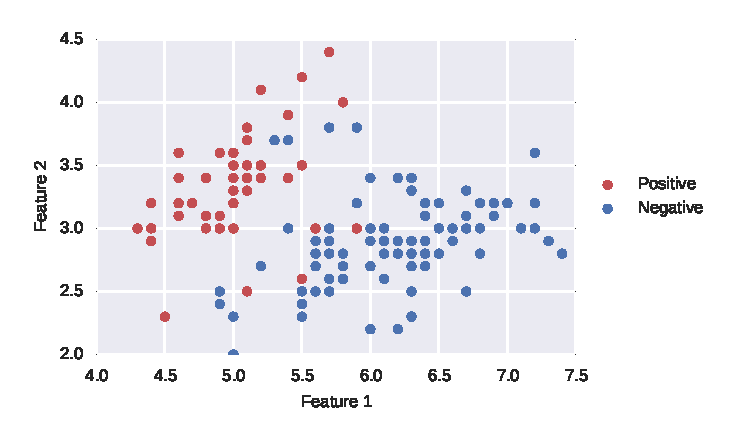
\includegraphics{ch2_fig1a}\label{fig:ch2:1a}}
\\
\subfloat[]{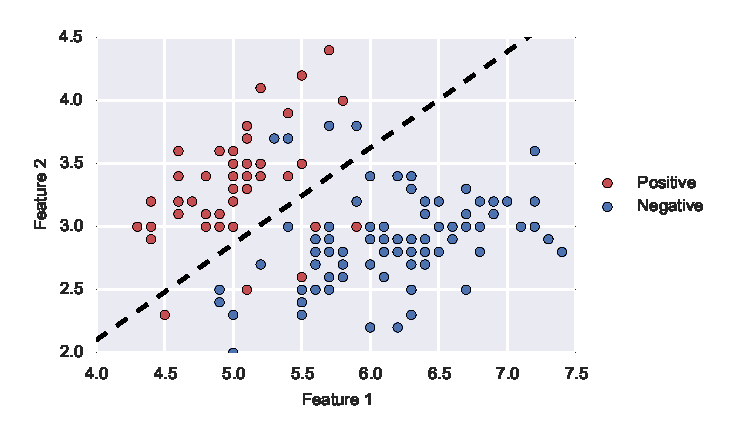
\includegraphics{ch2_fig1b}\label{fig:ch2:1b}}
\caption{Example of a classification algorithm. Using a set of examples from two classes, a 
	classification algorithm is learn in order to separate between the positives and the negatives. }
\label{fig:ch2:1}
\end{figure} 

There exists several algorithms that can be used for classification tasks. In general a 
classification algorithm is learn with the objective of finding patterns that separate between the 
different classes. In order to clarify this intuition, in \figurename{ \ref{fig:ch2:1}} an example 
of a classification algorithm is shown. Lets suppose a set of examples as shown in \figurename{ 
\ref{fig:ch2:1a}}.  Where the red points represents the positive examples and the blue the negative 
examples. The objective of a classifier is to find the best way to separate between the positive and 
negatives examples. In \figurename{ \ref{fig:ch2:1b}}, the output of a classifier learned using the 
set of examples is shown. It is observed that this classifier is able to separate almost all the 
examples using a linear classifier. 

However, not all examples are correctly classified. In particular there are 4 negative examples that 
were predicted as positive, and 5 positive examples that were predicted as negative. In the next 
section, we present the standard methods for evaluating the performance of a classification 
algorithm.

\begin{remark}{Classification examples}
Classification algorithms are widely used across a variety of domains. For example in the 
medical field, models have been used for making predictions about tumors, probability 
of a disease, selecting the right drug for a particular patient, and estimating the probability of 
relapsing, among others \citep{Herland2014}. In the financial sector, classification models have 
been successfully applied for fraud detection, credit scoring, portfolio management and algorithmic 
trading. Also, in marketing, several models are being currently used for churn modeling, customer 
targeting, behavior prediction and direct marketing \citep{Baesens2014}. Additionally, in many 
other emerging applications such as terrorism prevention, malware detection, computer security, 
energy consumption prediction, spam classification, and others \citep{Kriegel2007}.
\end{remark}

\subsection{Performance measures}

When evaluating the performance of a classification algorithm, the first thing to do is to check 
the number of examples that were misclassified. Since the the true class of the training examples 
is known. Therefore, evaluating the error of a model is as simply as counting the number of times 
an example is misclassified and divide it by the number of examples.

\begin{equation}\label{eqn:ch2:error}
Err(f({\cal S})) = \frac{1}{N}  \sum_{i=1}^N {\bf 1} _{y_i}(c_i),
\end{equation}
where $\mathbf{1}_c(z)$ is an indicator function that takes the value of one if $z \in c$ and 
zero if $z \notin c$. Moreover the accuracy is defined as the percentage of times the algorithm 
made the correct prediction
\begin{equation}\label{eqn:ch2:accuracy}
Acc(f({\cal S})) = 1- Err(f({\cal S})).
\end{equation}

However, just knowing these statistics is not enough to make decisions, as in many applications is 
important to know where the errors are coming from. In particular, the misclassified examples may 
belong only to one class, which may give interesting insights about the problem.
A way to observe the different errors is by looking to the confusion matrix.
As shown in \tablename{ \ref{tab:ch2:1}}, 
\todo{how to calculate TP, FP...}

	\begin{table}[!t]
		\centering
		\footnotesize
    \begin{tabular}{c|c|c}
      \multicolumn{3}{c}{}\\
			\multicolumn{1}{c|}{}  & Actual Positive& Actual Negative \\
			\multicolumn{1}{c|}{} & $y=1$& $y=0$ \\
			\hline
			Predicted Positive 		& \multirow{ 2}{*}{True Positive ($TP$)} & \multirow{ 
			2}{*}{False Positive ($FP$)} \\
			$c=1$ & &\\
			\hline
			Predicted Negative  	& \multirow{ 2}{*}{False Negative ($FN$)} & \multirow{ 
			2}{*}{True Positive ($TN$)} \\
			$c=0$ & &\\
		\end{tabular}
		\caption{Classification confusion matrix}
		\label{tab:ch2:1}
  \end{table}  

  	From this table several statistics are extracted. In particular:
	\begin{itemize}
		\item Recall = $\frac{TP}{TP+FN}$
		\item Precision = $\frac{TP}{TP+FP}$
		\item $F_1Score = 2\frac{Precision \cdot Recall}{Precision + Recall}$
	\end{itemize}


  
  	\begin{table}[!t]
		\centering
		\footnotesize
    \begin{tabular}{c|c|c}
      \multicolumn{3}{c}{}\\
			\multicolumn{1}{c|}{}  & Actual Positive& Actual Negative \\
			\multicolumn{1}{c|}{} & $y=1$& $y=0$ \\
			\hline
			Predicted Positive 		& \multirow{ 2}{*}{36} & \multirow{ 
			2}{*}{4} \\
			$c=1$ & &\\
			\hline
			Predicted Negative  	& \multirow{ 2}{*}{5} & \multirow{ 
			2}{*}{68} \\
			$c=0$ & &\\
		\end{tabular}
		\caption{Confusion matrix of the toy example}
		\label{tab:ch2:2}
  \end{table}  
  
  Calculating the different statistics for this example
  	\begin{itemize}
  	\item Error = $\frac{4+9}{36+4+9+68}=8\%$
		\item Recall = $\frac{TP}{TP+FN}$
		\item Precision = $\frac{TP}{TP+FP}$
		\item $F_1Score = 2\frac{Precision \cdot Recall}{Precision + Recall}$
	\end{itemize}
	
	In order to make a comparison, using the same example toy set, a new algorithm is learn. This 
time the algorithm made the correct prediction more often as shown in \figurename{ \ref{fig:ch2:2}}.

\begin{figure}[t!]
	\centering
	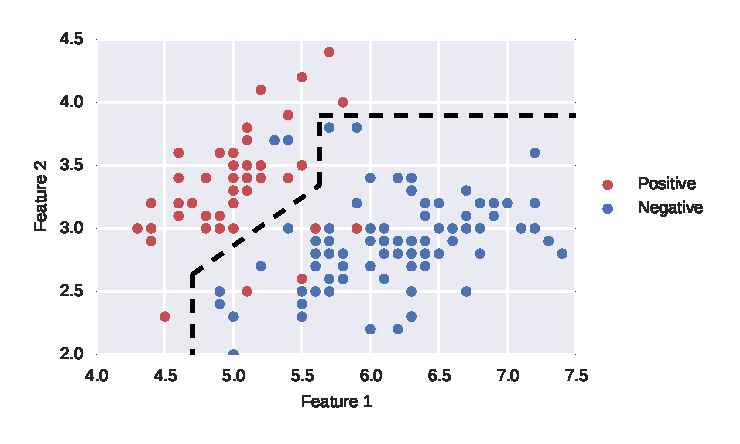
\includegraphics{ch2_fig2}
	\caption{Example of a classification algorithm. Using a set of examples from two classes, a 
	classification algorithm is learn in order to separate between the positives and the negatives. }
	\label{fig:ch2:2}
\end{figure}

    	\begin{table}[!t]
		\centering
		\footnotesize
    \begin{tabular}{c|c|c}
      \multicolumn{3}{c}{}\\
			\multicolumn{1}{c|}{}  & Actual Positive& Actual Negative \\
			\multicolumn{1}{c|}{} & $y=1$& $y=0$ \\
			\hline
			Predicted Positive 		& \multirow{ 2}{*}{37} & \multirow{ 
			2}{*}{2} \\
			$c=1$ & &\\
			\hline
			Predicted Negative  	& \multirow{ 2}{*}{4} & \multirow{ 
			2}{*}{70} \\
			$c=0$ & &\\
		\end{tabular}
		\caption{Confusion matrix of the toy example}
		\label{tab:ch2:2}
  \end{table}  
  Error = 5.31\%
  
\subsection{Families of binary classifiers}
% \subsection{Linear models}
% \subsection{Decision tree models}
% \subsection{Neural networks}
% \subsection{Suport vector machines}
% \subsection{Ensemble based classifiers}
% \section{Sampling}
% \subsection{Under/over sampling}
% \subsection{SMOTE}

% \chapter{Cost-sensitive classification}
% 
% \begin{remark}{Outline}
% \todo{fix outline}
% In this chapter, we present the well-known family of \textit{random forests}
% methods. In Section~\ref{sec:4:bias-variance}, we first describe the bias-variance
% decomposition of the prediction error and then present, in
% Section~\ref{sec:4:ensemble}, how aggregating randomized models through
% ensembles reduces the prediction error by decreasing the variance term in this
% decomposition. In Section~\ref{sec:4:random-forests}, we revisit random forests
% and its variants and study how randomness introduced into the decision trees
% reduces prediction errors by decorrelating the decision
% trees in the ensemble. Properties and features of random forests are then outlined
% in Section~\ref{sec:4:features} while their consistency
% is finally explored in Section~\ref{sec:4:consistency}.
% \end{remark}


\section{Cost-sensitive classification}
\todo{ Change notation}
  Classification, in the context of machine learning, deals with the problem of predicting the class
  of a set of examples given their features. Traditionally, classification methods aim at 
  minimizing the misclassification of examples, in which an example is misclassified if the 
  predicted class is different from the true class. Such a traditional framework assumes that all 
  misclassification errors carry the same cost. This is not the case in many real-world 
  applications. Methods that use different misclassification costs are known as cost-sensitive 
  classifiers. Typical cost-sensitive approaches assume a constant cost for each type of error, in 
  the sense that, the cost depends on the class and is the same among examples 
  \citep{Elkan2001,Kim2012}. 
  Although, this class-dependent approach is not realistic in many real-world applications, for 
  example in credit card fraud detection, failing to detect a fraudulent transaction may have an 
  economical impact from a few to thousands of Euros, depending on the particular transaction and 
  card holder \citep{Sahin2013}. In churn modeling, a model is used for predicting which
  customers are more likely to abandon a service provider. In this context, failing to identify a 
  profitable or unprofitable churner have a significant different financial impact 
  \citep{Glady2009}. Similarly, in direct marketing, wrongly predicting that a customer will not 
  accept an offer when in fact he will, has a different impact than the other way around 
  \citep{Zadrozny2003}. Also in credit scoring, where declining good customers has a non constant 
  impact since not all  customers generate the same profit \citep{Verbraken2014}. Lastly, in the 
  case of intrusion   detection, classifying a benign connection as malicious have a different cost 
  than when a   malicious connection is accepted \citep{Ma2011}.

  In order to deal with these specific types of cost-sensitive problems, called example-dependent
  cost-sensitive, some methods have been proposed recently. However, the literature on 
  example-dependent cost-sensitive methods is limited, mostly because there is a lack of publicly 
  available datasets that fit the problem \citep{MacAodha2013}. Standard solutions consist in 
  modifying the training set by re-weighting the examples proportionately to the misclassification 
  costs \citep{Elkan2001,Zadrozny2003}.

\subsection{Binary classification cost characteristic}
    In classification problems with two classes $y_i \in \{0,1\}$, the objective is to learn or 
    predict to which class $c_i \in \{0,1\}$ a given example $i$ belongs based on its $k$ features 
    $X_i=[x^1_i, x^2_i,...,x^k_i]$. In this context, classification costs can be represented using 
    a 2x2 cost matrix \citep{Elkan2001}, that introduces the costs associated with two types of 
    correct classification, true positives ($C_{TP_i}$), true negatives ($C_{TN_i}$), and the two 
    types of misclassification errors, false positives ($C_{FP_i}$), false negatives ($C_{FN_i}$),
    as defined below:
    \begin{table}[h]
      \caption{Classification cost matrix}
      \centering
      \begin{tabular}{c|c|c}
        \multicolumn{1}{c|}{}  & Actual Positive& Actual Negative \\
        \multicolumn{1}{c|}{} & $y_i=1$& $y_i=0$ \\
        \hline
        Predicted Positive    & \multirow{ 2}{*}{$C_{TP_i}$} & \multirow{ 2}{*}{$C_{FP_i}$} \\
        $c_i=1$ & &\\
        \hline
        Predicted Negative    & \multirow{ 2}{*}{$C_{FN_i}$} & \multirow{ 2}{*}{$C_{TN_i}$} \\
        $c_i=0$ & &\\
      \end{tabular}
    \end{table}  

  Conceptually, the cost of correct classification should always be lower than the cost of 
misclassification.
  These are referred to as the ``reasonableness`` conditions \citep{Elkan2001}, and are defined as
  $C_{FP_i} > C_{TN_i}$ and $C_{FN_i} > C_{TP_i}$.
  Taking into account the ``reasonableness`` conditions, a simpler cost matrix 
  with only one degree of freedom has been defined in \citep{Elkan2001},
  by scaling and shifting the initial cost matrix, resulting in:
  \begin{center}
  \begin{tabular}{c|c}

  \multirow{ 2}{*}{Negative} & \multirow{ 
2}{*}{$C^*_{FN_i}=\frac{(C_{FN_i}-C_{TN_i})}{(C_{FP_i}-C_{TN_i})}$} \\
  \\
  \hline
  \multirow{ 2}{*}{Positive} & \multirow{ 
2}{*}{$C^*_{TP_i}=\frac{(C_{TP_i}-C_{TN_i})}{(C_{FP_i}-C_{TN_i})}$} \\
  \\ 
  \end{tabular}
\end{center}

  A classification problem is said to be cost-insensitive if costs of both errors are equal. It 
    is class-dependent cost-sensitive if the costs are different but constant. Finally we talk 
    about an example-dependent cost-sensitive classification problem if the cost matrix is not 
    constant for all the examples.
  
    However, the definition above is not general enough. There are many cases when the cost matrix 
    is not constant and still the problem is cost-insensitive or class-dependent cost-sensitive. 
    For example, if the costs of correct classification are zero, \mbox{$C_{TP_i}=C_{TN_i}=0$}, 
    and the costs of misclassification are $C_{FP_i}=a_0\cdot z_i$ and $C_{FN_i}=a_1\cdot z_i$,
    where $a_0$, $a_1$, are constant and $z_i$ a random variable. This is an example of a cost 
    matrix that is not constant. However, $C^*_{FN_i}$ and $C^*_{TP_i}$ are constant, i.e. 
    $C^*_{FN_i}=(a_1\cdot z_i)/(a_0\cdot z_i)=a_1/a_0$ and $C^*_{TP_i}=0$ $\forall i$. In 
    this case the problem is cost-insensitive if $a_0=a_1$, or class-dependent cost-sensitive if 
    $a_0 \ne a_1$, even given the fact that the cost matrix is not constant.
  
    Nevertheless, using only the simpler cost matrix is not enough to define when a problem is 
    example-dependent cost-sensitive. To achieve this, we define the classification problem cost 
    characteristic as 
    \begin{equation}
     b_i = C^*_{FN_i}-C^*_{TP_i},
    \end{equation}
    and define its mean and standard deviation as $\mu_b$ and $\sigma_b$, respectively.
  
    Using $\mu_b$ and $\sigma_b$, we analyze different binary classification problems. In the case 
    of a cost-insensitive classification problem, for every example $i$ \mbox{$C_{FP_i}=C_{FN_i}$}
    and $C_{TP_i}=C_{TN_i}$, leading to $b_i=1$ $\forall i$ or more generally $\mu_b=1$ and 
    $\sigma_b=0$. For class-dependent cost-sensitive problems, the costs are not equal but 
    constants \mbox{$C_{FP_i}\ne C_{FN_i}$} or \mbox{$C_{TP_i}\ne C_{TN_i}$}, leading to $b_i \ne 
    1$ $\forall i$, or $\mu_b \ne 1$ and $\sigma_b=0$. Lastly, in the case of example-dependent 
    cost-sensitive problems, the cost difference is non constant or $\sigma_b \ne 0$.
  
    In summary a binary classification problem is defined according to the following conditions:
    \begin{table}[h]
      \centering
      \begin{tabular}{c | c | l}
        $\mu_b$ & $\sigma_b$ & Type of classification problem \\
        \hline 
        && \\
        $1$ &  $0$ & cost-insensitive \\ &&\\
        $\ne 1$ & $0$ & class-dependent cost-sensitive \\ &&\\
        & $\ne 0$ & example-dependent cost-sensitive \\ 
      \end{tabular}
    \end{table}

\subsection{Example-dependent Cost-based evaluation masures}
    Common cost-insensitive evaluation measures such as misclassification rate or \mbox{$F-Score$}, 
    assume the same cost for the different misclassification errors. Using these measures is not 
    suitable for example-dependent cost-sensitive binary classification problems. Indeed, two 
    classifiers with equal misclassification rate but different numbers of false positives and 
    false negatives do not have the same impact on cost since \mbox{$C_{FP_i}\ne C_{FN_i}$};
    therefore there is a need for a measure that takes into account the actual costs 
    ~$C_i=[C_{TP_i},C_{FP_i},C_{FN_i},C_{TN_i}]$ of each example $i$, as introduced in 
    the previous section.
  
    Let $S$ be a set of $N$ examples $i$, $N=\vert S \vert$, where each example is represented by 
    the augmented feature vector \mbox{$X^a_i=[X_i, C_i]$} and labelled using the class label $y_i 
    \in \{0,1\}$.
    A classifier $f$ which generates the predicted label $c_i$ for each element $i$ is trained 
    using the set $S$. Then the cost of using $f$ on $S$ is calculated by
    \begin{align}\label{eq:cost}
      Cost(f(S)) = \sum_{i=1}^{N} & {\bigg( y_i(c_i C_{TP_i} + (1-c_i)C_{FN_i})} + \\
      & {(1-y_i)(c_i C_{FP_i} + (1-c_i)C_{TN_i}) \bigg)}.
    \end{align}

However, the total cost may not be easy to interpret. In \citep{Whitrow2008}, a 
  \textit{normalized} cost measure was proposed, by dividing the total cost by the theoretical 
  maximum cost, which is the cost of misclassifying every example. The \textit{normalized} cost is 
  calculated using
  \begin{align}\label{eq:ncost}
    NCost(f(\mathcal{S})) = \frac{Cost(f(\mathcal{S}))}
    {\sum_{i \in \mathcal{S}_0} C_{FN_i} + 
    \sum_{i \in \mathcal{S}_1} C_{FP_i}},
  \end{align} 
  
  We proposed similar approach in \citep{CorreaBahnsen2014b}, where the savings of using an 
  algorithm  are defined as the cost of the algorithm versus the cost of using no algorithm at all. 
  To do that, the cost of the costless class is defined as 
  \begin{equation}
    Cost_l(\mathcal{S}) = \min \{Cost(f_0(\mathcal{S})), Cost(f_1(\mathcal{S}))\},
  \end{equation}
  where 
  \begin{equation}\label{eq:f_a}
    f_a(\mathcal{S}) = \mathbf{a}, \text{ with } a\in \{0,1\}.
  \end{equation}

  The cost improvement can be expressed as the cost savings as compared with $Cost_l(\mathcal{S})$. 
  \begin{equation}\label{eq:savings}
    Savings(f(\mathcal{S})) = \frac{ Cost_l(\mathcal{S}) - Cost(f(\mathcal{S}))}
    {Cost_l(\mathcal{S})}.
  \end{equation} 


\subsection{State-of-the-art methods}
\todo{Extend description of each method}

    As mentioned earlier, taking into account the different costs associated with each example, 
    some methods have been proposed to make classifiers example-dependent cost-sensitive. These 
    methods may be grouped in two categories. Methods based on changing the class distribution of 
    the training data, which are known as cost-proportionate sampling methods; and direct cost 
    methods \citep{Wang2013}.
  
    A standard method to introduce example-dependent costs into classification algorithms is to 
    re-weight the training examples based on their costs, either by cost-proportionate 
    rejection-sampling \citep{Zadrozny2003}, or over-sampling \citep{Elkan2001}. The 
    rejection-sampling approach consists in selecting a random subset $S_{r}$  by randomly 
    selecting examples from $S$, and accepting each example $i$ with probability $w_i/ 
    \max\limits_{1,\dots, N}\{w_i\}$, where $w_i$ is defined as the expected misclassification 
    error of example $i$:
    \begin{equation}\label{eq_pred1}
      w_i = y_i\cdot C_{FN_i}+(1-y_i)\cdot C_{FP_i}.
    \end{equation}
    Lastly, the over-sampling method consists in creating a new set $S_{o}$, by making $w_i$ 
    copies of each example $i$. However, cost-proportionate over-sampling increases the training 
    since $\vert S_{o}\vert >> \vert S \vert$, and it also may result in over-fitting 
    \citep{Drummond2003}. Furthermore, none of these methods uses the full cost matrix but only the 
    misclassification costs.

In addition to the traditional aforementioned algorithms we also evaluate a thresholding 
optimization to make the 
   classifiers cost sensitive, based on the method proposed in \cite{Sheng2006}.
   The idea behind this approach is to adaptively modify the probability threshold of an 
   algorithm such that a certain criterion is minimized; in our case the cost due to fraud.
   By default the probability threshold of an algorithm is 50\%, meaning that when the probability 
   of a positive event is greater than 50\% that example is classified as positive.
   This default threshold is not necessarily the one that minimizes the cost due to fraud. 
   %So we make an optimization, in the training dataset, in order to find the threshold which 
minimizes the cost measure,
   %and by doing so, we make the algorithm cost sensitive.
   So we make an optimization in the training dataset, in order to find the threshold which 
minimizes the cost measure.
   Then, this new threshold is applied to the test dataset to obtain the results,
   and by doing so, we make the algorithm cost sensitive by threshold optimization.\cleardoublepage
	\chapter{Cost-sensitive classification}\label{ch:3}

\begin{remark}{Outline}
In this chapter, we introduce classifications models from a machine learning perspective. 
Moreover, we present the example-dependent cost-sensitive framework that is the basis of the 
thesis. In Section~\ref{sec:3:classification}, we give a self contain introduction to 
classification, including the most-common algorithms, and the main methods for evaluating the 
performance of the different algorithm. Then, in Section~\ref{sec:3:cs}, we present the general 
framwork of cost-sensitive classification. Within this Section, we first introduce a method for 
defining the type of cost-sensitivity of a problem. Afterwards, we present the different 
cost-sensitive performance evaluation measures. Lastly, we show the state-of-the-art 
example-dependent cost-sensitive methods cost-proportionate rejection-sampling and 
cost-proportionate over-sampling.
\end{remark}


\section{Introduction}
\label{sec:3:intro}

  Classification, in the context of machine learning, deals with the problem of predicting the class
  of a set of examples given their features. Traditionally, classification methods aim at 
  minimizing the misclassification of examples, in which an example is misclassified if the 
  predicted class is different from the true class. Such a traditional framework assumes that all 
  misclassification errors carry the same cost. This is not the case in many real-world 
  applications. Methods that use different misclassification costs are known as cost-sensitive 
  classifiers. Typical cost-sensitive approaches assume a constant cost for each type of error, in 
  the sense that, the cost depends on the class and is the same among examples
  \citep{Elkan2001,Kim2012}. Although, this class-dependent approach is not realistic in many 
  real-world applications.
  
  \begin{remark}{Real-world cost sensitive applications}
  For example in credit card fraud detection, failing to detect a fraudulent transaction may have 
  an economical impact from a few to thousands of Euros, depending on the particular transaction 
  and card holder \citep{Sahin2013}. In churn modeling, a model is used for predicting which
  customers are more likely to abandon a service provider. In this context, failing to identify a 
  profitable or unprofitable churner have a significant different financial impact 
  \citep{Glady2009}. Similarly, in direct marketing, wrongly predicting that a customer will not 
  accept an offer when in fact he will, has a different impact than the other way around 
  \citep{Zadrozny2003}. Also in credit scoring, where declining good customers has a non constant 
  impact since not all  customers generate the same profit \citep{Verbraken2014}. Lastly, in the 
  case of intrusion   detection, classifying a benign connection as malicious have a different cost 
  than when a   malicious connection is accepted \citep{Ma2011}.
  \end{remark}

  In order to deal with these specific types of cost-sensitive problems, called example-dependent
  cost-sensitive, some methods have been proposed recently. However, the literature on 
  example-dependent cost-sensitive methods is limited, mostly because there is a lack of publicly 
  available datasets that fit the problem \citep{MacAodha2013}. Standard solutions consist in 
  modifying the training set by re-weighting the examples proportionately to the misclassification 
  costs \citep{Elkan2001,Zadrozny2003}.

  
\section{Class-dependent cost-sensitive classification}
\label{sec:3:class-dependent}

The cost-sensitive literature is mostly focused in class-dependent problems \citep{Elkan2001}, where 
the cost of misclassification is associated with the class. Ussually, the cost of misclassifying a 
positive example is denoted by $c_0$ and the one of misclassifying a negative example is denoted by 
$c_1$. Conceptually, $c_0\ge0$ and $c_1\ge0$, moreover, it is ussually defined that $c_0+c_1=2$ 
\citep{Flach2011a}, as when $c_0=c_1=1$ represents the case of cost-insensitive classification. 
Using the previous notation, a class-dependent cost measure is defined as \citep{Wang2014}:
\begin{equation}
  Cost_{cd}(f(\mathcal{S})) = c_0 \cdot FP + c_1 \cdot FN,
\end{equation}
where $FP$ and $FN$ are the number of false positives and false negatives, respectively.

Following the toy example shown in Section~\ref{sec:2:classification}, we now assume that 
misclassifying a negative example have a cost of $c_0=0.2$ and a positive example $c_1=1.8$. 
Under this scenario, the misclassifying a positive example have a much higher cost than 
misclassifying a negative one. Taking that into account, in \figurename{~\ref{fig:3:1}, we show an 
algorithm (Algorithm3), that focus on maximizing the correct classification of the positives, 
scarifying the correct classification of the negatives. In the following table, we compare the 
results of the standard measures and the class-dependent cost, of Algorithm3 and the classification 
algorithms presented in \figurename{~\ref{fig:2:2b}} (Algorithm1) and \figurename{ \ref{fig:2:3}} 
(Algorithm2):
\begin{center}
    \footnotesize
  \begin{tabular}{l|c|c|c|c|c}
  Algorithm & Error & Recall & Precision & $F_1Score$ & $Cost_{cd}$ \\
  \hline
  Algorithm1 & 11.11\% & 87.8\%& 90\%& 88.8\% & 9.8\\ %FP = 4 , FN=5
  Algorithm2 & 5.3\% & 90.2\%& 94.9\%& 92.5\% & 7.6\\ %FP = 2 , FN=4
  Algorithm3 & 7.97\%& 92.68\% &86.36\%& 89.41\% & 6.6 \\
  \end{tabular}
\end{center}

\begin{figure}[t!]
  \centering
  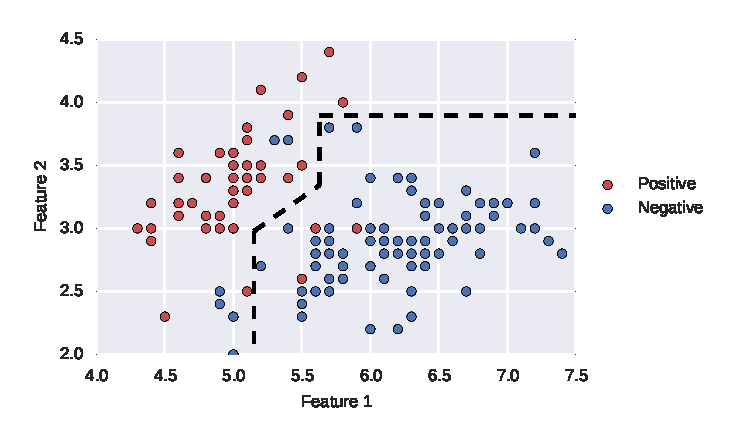
\includegraphics{ch3_fig1}
  \caption{Class-dependent cost-sensitive classification algorithm. Since the cost of misclassifying 
positives and negatives is different, the algorithm focus on maximizing the correct classification 
of the positives, scarifying the correct classification of the negatives.}
  \label{fig:3:1}
\end{figure}

It is found, that by focusing on the positives, Algorithm3 arises to a lower cost, even though, the 
traditional metrics are worst than Algorithm2. In conclusion, it is of highly importance to take 
into account the cost when evaluating and training a classification model.


\section{Example-dependent cost-sensitive classification}

The class-dependent framework introduced in the previous section, is highly restrictive, as 
assuming that the different costs are constant between classes is not realistic in many real world 
applications. In fraud detection, fraudulent transactions  can have a financial impact from 
hundreds or thousands of Euros \cite{Sahin2013}.


\section{Binary classification cost characteristic}
\label{sec:3:cost_characteristic}

  In classification problems with two classes $y_i \in \{0,1\}$, the objective is to learn or 
  predict to which class $c_i \in \{0,1\}$ a given example $i$ belongs based on its $k$ features 
  $\mathbf{x}_i=[x^1_i, x^2_i,...,x^k_i]$. In this context, classification costs can be 
  represented using a 2x2 cost matrix \citep{Elkan2001}, that introduces the costs 
  associated with   two types of correct   classification, true positives ($C_{TP_i}$), true 
  negatives ($C_{TN_i}$),   and the two  types of   misclassification errors, false positives 
  ($C_{FP_i}$), false negatives   ($C_{FN_i}$), as   defined in \tablename{ 
  \ref{tab:3:cost_matrix}}.

  
  \begin{table}[t]
    \centering
    \footnotesize
    \begin{tabular}{c|c|c}
      \multicolumn{1}{c|}{}  & Actual Positive& Actual Negative \\
      \multicolumn{1}{c|}{} & $y_i=1$& $y_i=0$ \\
      \hline
      Predicted Positive    & \multirow{ 2}{*}{$C_{TP_i}$} & \multirow{ 2}{*}{$C_{FP_i}$} \\
      $c_i=1$ & &\\
      \hline
      Predicted Negative    & \multirow{ 2}{*}{$C_{FN_i}$} & \multirow{ 2}{*}{$C_{TN_i}$} \\
      $c_i=0$ & &\\
    \end{tabular}
    \caption{Classification cost matrix}
    \label{tab:3:cost_matrix}
  \end{table}  

  Conceptually, the cost of correct classification should always be lower than the cost of 
  misclassification. These are referred to as the ``reasonableness`` conditions \citep{Elkan2001}, 
  and are defined as  $C_{FP_i} > C_{TN_i}$ and $C_{FN_i} > C_{TP_i}$.
  Taking into account the ``reasonableness`` conditions, a simpler cost matrix 
  with only one degree of freedom has been defined in \citep{Elkan2001},
  by scaling and shifting the initial cost matrix, resulting in:
  \begin{center}
    \footnotesize
    \begin{tabular}{c|c}
    \multirow{ 2}{*}{Negative} & \multirow{ 
    2}{*}{$C^*_{FN_i}=\frac{(C_{FN_i}-C_{TN_i})}{(C_{FP_i}-C_{TN_i})}$} \\
    \\
    \hline
    \multirow{ 2}{*}{Positive} & \multirow{ 
    2}{*}{$C^*_{TP_i}=\frac{(C_{TP_i}-C_{TN_i})}{(C_{FP_i}-C_{TN_i})}$} \\
    \\ 
    \end{tabular}
  \end{center}

  A classification problem is said to be cost-insensitive if costs of both errors are equal. It 
  is class-dependent cost-sensitive if the costs are different but constant. Finally we talk 
  about an example-dependent cost-sensitive classification problem if the cost matrix is not 
  constant for all the examples.

  However, the definition above is not general enough. There are many cases when the cost matrix 
  is not constant and still the problem is cost-insensitive or class-dependent cost-sensitive. 
  For example, if the costs of correct classification are zero, $C_{TP_i}=C_{TN_i}=0$, 
  and the costs of misclassification are $C_{FP_i}=a_0\cdot z_i$ and $C_{FN_i}=a_1\cdot z_i$,
  where $a_0$, $a_1$, are constant and $z_i$ a random variable. This is an example of a cost 
  matrix that is not constant. However, $C^*_{FN_i}$ and $C^*_{TP_i}$ are constant, i.e. 
  $C^*_{FN_i}=(a_1\cdot z_i)/(a_0\cdot z_i)=a_1/a_0$ and $C^*_{TP_i}=0$ $\forall i$. In 
  this case the problem is cost-insensitive if $a_0=a_1$, or class-dependent cost-sensitive if 
  $a_0 \ne a_1$, even given the fact that the cost matrix is not constant.

  Nevertheless, using only the simpler cost matrix is not enough to define when a problem is 
  example-dependent cost-sensitive. To achieve this, we proposed in \citep{CorreaBahnsen2015}, 
  the classification problem cost characteristic as:
  \begin{equation}
    b_i = C^*_{FN_i}-C^*_{TP_i},
  \end{equation}
  and define its mean and standard deviation as $\mu_b$ and $\sigma_b$, respectively.

  Using $\mu_b$ and $\sigma_b$, we analyze different binary classification problems. In the case 
  of a cost-insensitive classification problem, for every example $i$ \mbox{$C_{FP_i}=C_{FN_i}$}
  and $C_{TP_i}=C_{TN_i}$, leading to $b_i=1$ $\forall i$ or more generally $\mu_b=1$ and 
  $\sigma_b=0$. For class-dependent cost-sensitive problems, the costs are not equal but 
  constants \mbox{$C_{FP_i}\ne C_{FN_i}$} or \mbox{$C_{TP_i}\ne C_{TN_i}$}, leading to $b_i \ne 
  1$ $\forall i$, or $\mu_b \ne 1$ and $\sigma_b=0$. Lastly, in the case of example-dependent 
  cost-sensitive problems, the cost difference is non constant or $\sigma_b \ne 0$.

  In summary a binary classification problem is defined according to the following conditions:
  \begin{center}
    \footnotesize
    \begin{tabular}{c | c | l}
      $\mu_b$ & $\sigma_b$ & Type of classification problem \\
      \hline 
      && \\
      $1$ &  $0$ & cost-insensitive \\ &&\\
      $\ne 1$ & $0$ & class-dependent cost-sensitive \\ &&\\
      & $\ne 0$ & example-dependent cost-sensitive \\ 
    \end{tabular}
  \end{center}
  

\subsection{Example-dependent evaluation measures}
\label{sec:3:csmeasures}

  Common cost-insensitive evaluation measures such as misclassification rate or \mbox{$F_1Score$}, 
  assume the same cost for the different misclassification errors. Using these measures is not 
  suitable for example-dependent cost-sensitive binary classification problems. Indeed, two 
  classifiers with equal misclassification rate but different numbers of false positives and 
  false negatives do not have the same impact on cost since \mbox{$C_{FP_i}\ne C_{FN_i}$};
  therefore there is a need for a measure that takes into account the actual costs 
  $\{C_{TP_i},C_{FP_i},C_{FN_i},C_{TN_i}\}$ of each example $i$, as introduced in the previous 
  Section.
  \label{ntn:ch2:3}

  Let $\mathcal{S}$ be a set of $N$ examples $i$, $N=\vert S \vert$, where each example is 
  represented by  the augmented feature vector $\mathbf{x}_i^*=[\mathbf{x}_i, 
  C_{TP_i},C_{FP_i},C_{FN_i},C_{TN_i}]$  and labeled using the class   label $y_i   \in \{0,1\}$. 
  A classifier $f$ which generates the   predicted label $c_i$ for each   element $i$ is trained  
  using the set $\mathcal{S}$. Then the cost of   using $f$ on $\mathcal{S}$ is calculated by
  \begin{equation}\label{eq:3:cost_total}
     Cost(f(\mathcal{S})) = \sum_{i=1}^N Cost(f(\mathbf{x}_i^*)),
  \end{equation}
  where
   \begin{align}\label{eq:3:cost}
    Cost(f(\mathbf{x}_i^*)) =& y_i(c_i C_{TP_i} + (1-c_i)C_{FN_i}) + \nonumber \\  
    & (1-y_i)(c_i C_{FP_i} + (1-c_i)C_{TN_i}).
  \end{align}

  However, the total cost may not be easy to interpret. In \citep{Whitrow2008}, a 
  \textit{normalized} cost measure was proposed, by dividing the total cost by the theoretical 
  maximum cost, which is the cost of misclassifying every example. The \textit{normalized} cost is 
  calculated using
  \begin{align}\label{eq:3:ncost}
    Cost_n(f(\mathcal{S})) = \frac{Cost(f(\mathcal{S}))}
    {\sum_{i=1}^N C_{FN_i} \cdot \mathbf{1}_0(y_i) 
    +  C_{FP_i} \cdot \mathbf{1}_1(y_i)  }.
  \end{align} 

  We proposed similar approach in \citep{CorreaBahnsen2014b}, where the savings of using an 
  algorithm  are defined as the cost of the algorithm versus the cost of using no algorithm at all. 
  To do that, the cost of the costless class is defined as 
  \begin{equation}
    Cost_l(\mathcal{S}) = \min \{Cost(f_0(\mathcal{S})), Cost(f_1(\mathcal{S}))\},
  \end{equation}
  where 
  \begin{equation}\label{eq:3:f_a}
    f_a(\mathcal{S}) = \mathbf{a}, \text{ with } a\in \{0,1\}.
  \end{equation}

  The cost improvement can be expressed as the cost savings as compared with $Cost_l(\mathcal{S})$. 
  \begin{equation}\label{eq:3:savings}
    Savings(f(\mathcal{S})) = \frac{ Cost_l(\mathcal{S}) - Cost(f(\mathcal{S}))}
    {Cost_l(\mathcal{S})}.
  \end{equation} 


\subsection{State-of-the-art methods}

  As mentioned earlier, taking into account the different costs associated with each example, 
  some methods have been proposed to make classifiers example-dependent cost-sensitive. These 
  methods may be grouped in two categories. Methods based on changing the class distribution of 
  the training data, which are known as cost-proportionate sampling methods; and direct cost 
  methods \citep{Wang2013}.

  A standard method to introduce example-dependent costs into classification algorithms is to 
  re-weight the training examples based on their costs, either by cost-proportionate 
  rejection-sampling \citep{Zadrozny2003}, or over-sampling \citep{Elkan2001}. The 
  rejection-sampling approach consists in selecting a random subset $\mathcal{S}_{r}$  by 
  randomly  selecting examples from $\mathcal{S}$, and accepting each example $i$ with 
  probability $w_i/ \max\limits_{1,\dots, N}\{w_i\}$, where $w_i$ is defined as the expected 
  misclassification error of example $i$:
  \begin{equation}\label{eq_pred1}
    w_i = y_i\cdot C_{FN_i}+(1-y_i)\cdot C_{FP_i}.
  \end{equation}
  Lastly, the over-sampling method consists in creating a new set $\mathcal{S}_{o}$, by making 
  $w_i$ copies of each example $i$. However, cost-proportionate over-sampling increases the 
  training  since $\vert \mathcal{S}_{o}\vert >> \vert \mathcal{S} \vert$, and it also may result 
  in over-fitting  \citep{Drummond2003}. Furthermore, none of these methods uses the full cost 
  matrix but only the  misclassification costs.

  The second approach, consists in using the predicted probability $\hat p_i$, estimated using a 
  given classifier $f$, and   modify the threshold $t$  such that the savings are maximized. 
  This method is called cost-sensitive thresholding \citep{Sheng2006}. The idea behind this 
approach 
  is to adaptively modify the probability threshold of an algorithm $f_t$ in order to maximized the 
  savings of the algorithm on a given set $Savings(f^t(\mathcal{S}))$. The threshold is calculated 
  using the following equation
  \begin{equation}
   t_{thresholding} = \argmax_t Savings(f^t(\mathcal{S})).
  \end{equation}

  \cleardoublepage


\ctparttext{You can put some informational part preamble text here. 
Illo principalmente su nos. Non message \emph{occidental} angloromanic
da. Debitas effortio simplificate sia se, auxiliar summarios da que,
se avantiate publicationes via. Pan in terra summarios, capital
interlingua se que. Al via multo esser specimen, campo responder que
da. Le usate medical addresses pro, europa origine sanctificate nos se.}
\part{Real-world applications}
\todo{intro part 2}

	\chapter{Financial risk modeling}\label{ch:4}

\begin{remark}{Outline}
In this chapter, we present two different real-world example-dependent 
cost-sensitive problems related to financial risk modeling, namely, credit card fraud detection and 
credit scoring. Both problems are example-dependent cost-sensitive, as failing to identify a 
fraudulent transaction may have a financial impact ranging from tens to thousands of Euros. 
Similarly in credit scoring, approving a customer that later does not pay his debt has a 
significant impact on a bank profit. First, in Section~\ref{sec:4:fraud},  we introduce the credit 
card fraud detection problem and present our propose periodic features.  Lastly in 
Section~\ref{sec:4:creditscoring}, the credit scoring problem is presented and we propose a new 
financial evaluation measure for credit scoring.
\end{remark}

\section{Credit card fraud detection}
\label{sec:4:fraud}

  The use of credit and debit cards has increased significantly   in the last years, unfortunately 
  so has the fraud. Because of that, billions of Euros are lost every year. According to 
  the European Central Bank \citep{EuropeanCentralBank2013}, during 2012 the total level of fraud 
  reached 1.33 billion Euros in the Single Euro Payments Area, which represents an increase of 
  14.8\% compared with 2011. Moreover, payments across non traditional channels (mobile, internet, 
  ...) accounted for 60\% of the fraud, whereas it was 46\% in 2008. This opens new challenges as 
  new fraud patterns emerge, and current fraud detection systems are not being successful in 
  preventing fraud. Furthermore, fraudsters constantly change their strategies to avoid being 
  detected, something that makes traditional fraud detection tools such as expert rules inadequate.
  
  The use of machine learning in fraud detection has been an interesting topic in recent years. 
  Several detection systems based on machine learning techniques have been successfully used 
  for this problem \citep{Bhattacharyya2011}. When constructing a credit card fraud detection 
  model, there are several problems that have an important impact during the training phase: 
  Skewness of the data, cost-sensitivity of the application, short time response of the system, 
  dimensionality  of the search space and how to preprocess the features
  \citep{Bolton2002,Gadi2008,Whitrow2008,DalPozzolo2014,VanVlasselaer2015a}.  We are interested 
  in addressing the cost-sensitivity and the features preprocessing   issues. 
  
  Credit card fraud detection is by definition a cost-sensitive problem, in the sense that the 
  cost  due to a false positive is different than the cost of a false negative. When predicting a   
  transaction   as fraudulent, when in fact it is not a fraud, there is an administrative cost that 
  is incurred by  the financial institution. On the other hand, when failing to detect a fraud, the 
  amount of that  transaction is lost \citep{Hand2007a}. Moreover, it is not enough  to assume a  
  constant cost   difference between false positives and false negatives, as the amount of the  
  transactions varies   quite significantly; therefore, its financial impact is not constant but  
  depends on each   transaction. 
  
  When constructing a credit card fraud detection model, it is very important to use those features 
  that will help the algorithm make the best decision. Typical models only use raw transactional 
  features, such as time, amount, place of the transaction. However, these approaches does not take 
  into account the spending behavior of the customer, which is expected to help discover fraud 
  patterns \citep{Gadi2008}. A standard way to include these behavioral spending patters was 
  proposed in \citep{Whitrow2008}, where Whitrow et al. proposed a transaction aggregation strategy 
  in order to take   into account a customer spending behavior. The derivation of the aggregated 
  features consists in grouping the transactions made during the last given number of hours, first 
  by card or account number, then by transaction type, merchant group, country or other, followed 
  by calculating  the number of transactions or the total amount spent on those transactions.
	
	In this section,  we first present a new cost-based measure to evaluate   credit card fraud 
  detection models, taking into account the different financial costs incurred by   the fraud 
  detection process. Afterwards, we propose an expanded version of the transaction 
  aggregation strategy, by  incorporating a combination criteria when grouping transactions, i.e., 
  instead of aggregating only  by card holder and transaction type, we combine it with 
  country or merchant group. This allows to have a much richer feature space. Moreover, we are 
  interested in analyzing the impact of adding the time of a transaction. The logic behind it, is 
  that a customer is expected to make transactions at similar hours. We, hence, propose a new 
  method for creating features  based on the  periodic behavior of a transaction time, using the 
  von Mises distribution \citep{Fisher1996}. In particular, these new time features should estimate 
  if the time of a new transaction is within the confidence interval of the  previous transaction 
  time. Furthermore, we present the real credit card fraud dataset 
  provided  by a large European card processing company used for the experiments in this 
  thesis.
  
  
\subsection{Credit card fraud detection evaluation}
\label{sec:4:frad:eval}

  A credit card fraud detection algorithm consists in identifying those transactions with a 
  high probability of being fraud, based on historical fraud patterns. The use of machine learning 
  in fraud detection has been an interesting topic in recent years. Different detection systems 
  that are based on machine learning  techniques have been successfully   used for this problem, in 
  particular: neural networks~\citep{Maes2002}, Bayesian learning \citep{Maes2002}, artificial 
  immune systems \citep{Gadi2008}, association rules \citep{Sanchez2009}, hybrid models 
  \citep{Krivko2010}, support vector machines~\citep{Bhattacharyya2011}, peer group  analysis 
  \citep{Weston2008}, online learning   
\citep{DalPozzolo2014}, discriminant analysis \citep{Mahmoudi2015} and social network analysis 
\citep{VanVlasselaer2015a}.
 
  Most of these studies compare their proposed algorithm with a benchmark algorithms and then make 
  the comparison using a standard binary classification measure, such as misclassification error, 
  receiver operating characteristic ($ROC$), Kolmogorov-Smirnov ($KS$) or \mbox{$F_1Score$} 
  statistics \citep{Bolton2002,Hand2007a,DalPozzolo2014}. 
  However, these measures may be not the most appropriate evaluation criteria when  evaluating 
  fraud detection models, because they tacitly assume that misclassification errors carry the same 
  cost, similarly with the correct classified transactions. This assumption does not hold in 
  practice, since  wrongly predicting a fraudulent transaction as legitimate carries a 
  significantly different financial cost than the inverse case. Furthermore, the accuracy measure 
  also assumes that the class distribution among transactions is constant and balanced 
  \citep{Provost1998}, and typically the distributions of a fraud detection dataset are skewed, 
  with a percentage of frauds ranging from 0.005\% to 0.5\% \citep{Gadi2008,Bhattacharyya2011}.
  
	In order to take into account the different costs of fraud detection during the evaluation of an 
	algorithm, we may use the cost matrix defined in \tablename{~\ref{tab:3:cost_matrix}}.
  Hand et al. \citep{Hand2007a} proposed a cost matrix, where in the case of false positive the 
  associated  cost is the administrative cost $C_{FP_i}=C_a$ related to analyzing the transaction 
  and contacting  the card holder. This cost is the same assigned to a true positive 
  $C_{TP_i}=C_a$, because in  this case,  the card holder will have to be contacted. However, in 
  the case of a false negative, in which a  fraud is  not detected, the cost is defined to be a 
  hundred times larger, i.e. $C_{FN_i}=100C_a$. This same approach was also used in 
  \citep{Gadi2008}.

  Nevertheless, in  practice, losses due to a specific fraud  range from few to 
  thousands of Euros, which means that  assuming constant cost for false  negatives is  
  unrealistic. In order to address this limitation, we   propose a 
  cost matrix that takes into account the actual  example-dependent financial costs. Our  cost 
  matrix defines the cost of a false negative to be the   amount $C_{FN_i}=Amt_i$ of the  
  transaction $i$. We argue that this cost matrix is a better representation of the   actual costs, 
  since when a  fraud is not detected, the losses of that particular fraud correspond   to the 
  stolen amount. The costs are summarized in \tablename{~\ref{tab:4:table_costmat_fraud}}.

	Afterwards, using (\ref{eq:3:cost}) a cost measure for fraud detection is calculated as:
  \begin{align} \label{eq:4:cost}
    Cost(f(\mathcal{S})) = \sum_{i=1}^{N} y_i(1-c_i)Amt_i + c_iC_a,
  \end{align}
  then, the savings of an algorithm are calculated using (\ref{eq:3:savings}).

	\begin{table}[t]
		\centering
		\footnotesize
		\begin{tabular}{c | c | c }
		\multicolumn{3}{c}{}\\
			\multicolumn{1}{c|}{}  & Actual Positive& Actual Negative \\
			\multicolumn{1}{c|}{} & $y_i=1$& $y_i=0$ \\
			\hline
			Predicted Positive 		& \multirow{ 2}{*}{$C_{TP_i}=C_a$} & \multirow{ 2}{*}{$C_{FP_i}=C_a$} 
			\\
			$c_i=1$ & &\\
			\hline
			Predicted Negative  	& \multirow{ 2}{*}{$C_{FN_i}=Amt_i$} & \multirow{ 
			2}{*}{$C_{TN_i}=0$} \\
			$c_i=0$ & &\\
			%\hline
		\end{tabular}
		\caption{Credit card fraud cost matrix}
		\label{tab:4:table_costmat_fraud}
	\end{table}
	 
\subsection{Feature engineering for fraud detection}
\label{sec:4:frad:features}

  When constructing a credit card fraud detection algorithm, the initial set of features (raw 
  features) include information regarding individual transactions. It is observed throughout the 
  literature, that regardless of the study, the set of raw features is quite similar. This is 
  because the data collected during a credit card transaction must comply with international 
  financial   reporting standards \citep{Aicpa2011}. In \tablename{~\ref{tab:4:raw_features}}, the 
  typical credit card fraud detection  raw features are summarized.
	
\subsubsection{Customer spending patterns}
\label{sec:4:frad:features_agg}
  
  Several studies use only the raw features in carrying  their analysis 
  \citep{Brause1999a,Minegishi2011,Panigrahi2009,Sanchez2009}. However, as noted in 
  \citep{Bolton2001}, a single transaction information is not sufficient to detect a fraudulent 
  transaction, since using only the raw features leaves behind important information such as 
  the consumer spending behavior, which is usually used by commercial fraud detection systems  
  \citep{Whitrow2008}.
  
	\begin{table}[!t]
   \centering
   \footnotesize
   \begin{tabular}{l l}
   \hline
   \textbf{Attribute name} & \textbf{Description}\\
   \hline
		Transaction ID & Transaction identification number \\
   Time & Date and time of the transaction\\
   Account number & Identification number of the customer\\
   Card number & Identification of the credit card\\
   Transaction type & ie. Internet, ATM, POS, ...\\
	 Entry mode & ie. Chip and pin, magnetic stripe, ...\\
   Amount & Amount of the transaction in Euros\\
   Merchant code & Identification of the merchant type\\
   Merchant group & Merchant group identification\\
   Country & Country of trx\\
   Country 2 & Country of residence \\
   Type of card & ie. Visa debit, Mastercard, American Express...\\
   Gender & Gender of the card holder\\
   Age & Card holder age\\
   Bank & Issuer bank of the card\\
   \hline
   \end{tabular}
   \caption{Summary of typical raw credit card fraud detection features}
   \label{tab:4:raw_features}
   \end{table}
	
  To deal with this, in \citep{Gadi2008}, a new set of features were proposed such that the 
  information of the last transaction made with the same credit card is also used to make a 
  prediction. The objective, is to be able to detect very dissimilar continuous transactions within 
  the purchases of a customer. The new set of features include: time since the last transaction, 
  previous  amount of the transaction, previous country of the transaction. Nevertheless, these 
  features do not take into account consumer behavior other than the last transaction made by a 
  client, this leads to having an incomplete profile of customers.
	
	A more compressive way to take into account a customer spending behavior is to derive some 
	features using a transaction aggregation strategy. This methodology was initially proposed in 
	\citep{Whitrow2008}.  The derivation of the aggregation features consists in  grouping 
	the transactions made during the last given number of hours, first by card or account number, 
	then by transaction type, merchant group, country or other, followed by calculating the number 
	of transactions or the total amount spent on those 	transactions. This methodology has been used 
	by a number of studies 
	\citep{Bhattacharyya2011,Weston2008,Tasoulis2008,CorreaBahnsen2013,Sahin2013,CorreaBahnsen2014,
DalPozzolo2014}.
	
  When aggregating a customer transactions, there is an important question on how much to 
  accumulate, in the sense that the marginal value of new information may diminish as time passes.
  \cite{Whitrow2008} discuss that aggregating 101 transactions is not likely to be
  more informative than aggregating 100 transactions. Indeed, when time passes, information lose 
  their value, in the sense that a customer spending patterns are not expected to remain constant 
  over the years. In particular, Whitrow et al. define a fixed time frame to be 24, 60 or 168 
  hours.
  
  The process of aggregating features consists in  selecting those transactions that were made in 
  the previous $t_p$ hours, for each transaction $i$ in the dataset $\mathcal{S}$,
	\begin{align}\label{eq:4:agg_features1}
	\mathcal{S}_{agg} \equiv	TRX_{agg}(\mathcal{S},& i, t_p) = \bigg\{x_l^{amt} \bigg\vert 
\left(x_l^{id}=x_i^{id}\right) \nonumber \\
		&\wedge \left(hours(x_i^{time},x_l^{time}) < t_p\right) \bigg\}_{l=1}^N,
	\end{align}
  where $N=\vert\mathcal{S}\vert$, $\vert \cdot \vert$ being the cardinality of a set, $x_i^{time}$ 
  is the time of transaction $i$,  $x_i^{amt}$ is the amount of transaction $i$, $x_i^{id}$  the 
  customer identification number of transaction $i$, and $hours(t_1,t_2)$ is  a function that 
  calculates the number of hours between the times $t_1$  and $t_2$. Afterwards the feature number 
  of transactions and amount of transactions in the last $t_p$ hours are calculated as:
  \begin{equation}\label{eq:4:agg1a}
    x_i^{a1} = \vert \mathcal{S}_{agg} \vert ,
  \end{equation}
  and   
  \begin{equation}\label{eq:4:agg1b}
  x_i^{a2} = \sum_{x^{amt} \in   \mathcal{S}_{agg} } x^{ amt},
  \end{equation}
  respectively.
	
  We note that this aggregation is not enough, in the sense that the combination 
  of  different features is not being taken into account. For example, it is not only 
  interesting   to see the total transactions, but also group them following a certain criteria, 
  such as: transactions   made in the last $t_p$ hours, in the same country   and of the same 
  transaction type. For   calculating such features, first we expand (\ref{eq:4:agg_features1}) as 
  follows
	\begin{align}\label{eq:4:agg_features2}
		\mathcal{S}_{agg2} \equiv & TRX_{agg}(\mathcal{S}  ,i, t_p, cond_1, cond_2) = \bigg\{ x_l^{amt} 
\bigg\vert \nonumber \\  
		& \left(x_l^{id}=x_i^{id}\right) \wedge  \left(hours(x_i^{time},x_l^{time})<  t_p\right) 
    \wedge \nonumber \\ 	
    &  \left(x_l^{cond_1} = x_i^{cond_1}\right) \wedge	\left(x_l^{cond_2} = 
		x_i^{cond_2}\right) \bigg\}_{l=1}^N.
		\end{align}
  where, $cond_1$ and $cond_2$, could be either of the features of a transaction listed in 
  \tablename{~\ref{tab:4:raw_features}}. Then, the features are calculated as:
  \begin{equation}\label{eq:4:agg2a}
     x_i^{a3} = \vert \mathcal{S}_{agg2} \vert ,
  \end{equation}
  and   
  \begin{equation}\label{eq:4:agg2b}
  x_i^{a4} = \sum_{x^{amt} \in   \mathcal{S}_{agg2}} x^{ amt}.
  \end{equation}

  To further clarify how the aggregated features are calculated we show an example. Consider a set 
  of transactions made by a client between the first and third of January of 2015, as shown in 
  \tablename{~\ref{tab:4:agg_features_example1}}. Then we estimate the aggregated features 
  ($x_i^{a1}$, $x_i^{a2}$, $x_i^{a3}$ and $x_i^{a4}$) by setting $t_p=24$ hours. The 
  different aggregated features give us different information of the customer spending   behavior. 
  Moreover, the total number of aggregated features can grow quite quickly, as $t_p$   can have   
  several values, and the combination of combination criteria can be quite large as well.
  In this thesis, we use a total of 280 aggregated features. In particular we set the 
  different values of $t_p$ to: 1, 3, 6, 12, 18, 24, 72 and 168 hours. Then calculate the 
  aggregated features   using (\ref{eq:4:agg_features1}), and also using (\ref{eq:4:agg_features2}) 
  with the following  grouping criteria:  country, type of transaction, entry mode, merchant code 
  and merchant group.
  
	\begin{table}[!t]
		\centering
    \footnotesize
   \begin{tabular}{|c c c c c | c c c c|}
   \hline
   \multicolumn{5}{|c|}{\textbf{Raw features}} & \multicolumn{4}{c|}{\textbf{Aggregated features}} 
		\\  \hline
   \textbf{Id} &\textbf{Time} & \textbf{Type} & \textbf{Country} & 
	\textbf{Amt} 		& $\mathbf{x}_i^{a1}$& $\mathbf{x}_i^{a2}$ & $\mathbf{x}_i^{a3}$ & 
$\mathbf{x}_i^{a4}$\\
   \hline
		1&  01/01 18:20& POS & LUX & 250 & 0 & 0  & 0 & 0\\
		2& 01/01 20:45& POS & LUX & 400 & 1 & 250& 1 & 250\\
		3& 01/01 22:40& ATM & LUX & 250 & 2 & 650& 0 & 0\\
		4&02/01 00:50& POS & GER & 50 		& 3 & 900& 0& 0\\
		5& 02/01 19:18& POS & GER & 100 	  & 3 & 700& 1& 50\\
		6& 02/01 23:45& POS & GER & 150 	  & 2 & 150& 2& 150\\
		7& 03/01 06:00& POS & LUX & 10  & 3 & 400& 0& 0\\
   \hline
   \end{tabular}
		\caption{Example calculation of aggregated features. For all aggregated features $t_p=24$.}
		\label{tab:4:agg_features_example1}
  \end{table}
	
	\subsubsection{Time features}
	\label{sec:4:frad:features_time}
	
  When using the aggregated features, there is still some information that is not completely 
  captured by those features. In particular we are interested in analyzing the time of the 
  transaction. The logic behind this, is that a customer is expected to make transactions at 
  similar hours. The issue when dealing with the time of the transaction, 
  specifically, when analyzing a feature such as the mean of transactions time, is that it is easy 
  to make the mistake of using the arithmetic mean. Indeed, the arithmetic mean is not a correct 
  way to average time because, as shown in \figurename{~\ref{fig:4:von1}}, it does not take into 
  account the periodic behavior of the time feature. For example, the arithmetic mean of 
  transaction time of four transactions made at 2:00, 3:00, 22:00 and 23:00 is 12:30, which is 
  counter intuitive since no transaction was made close to that time.

  \begin{figure}[!t]
  \centering
  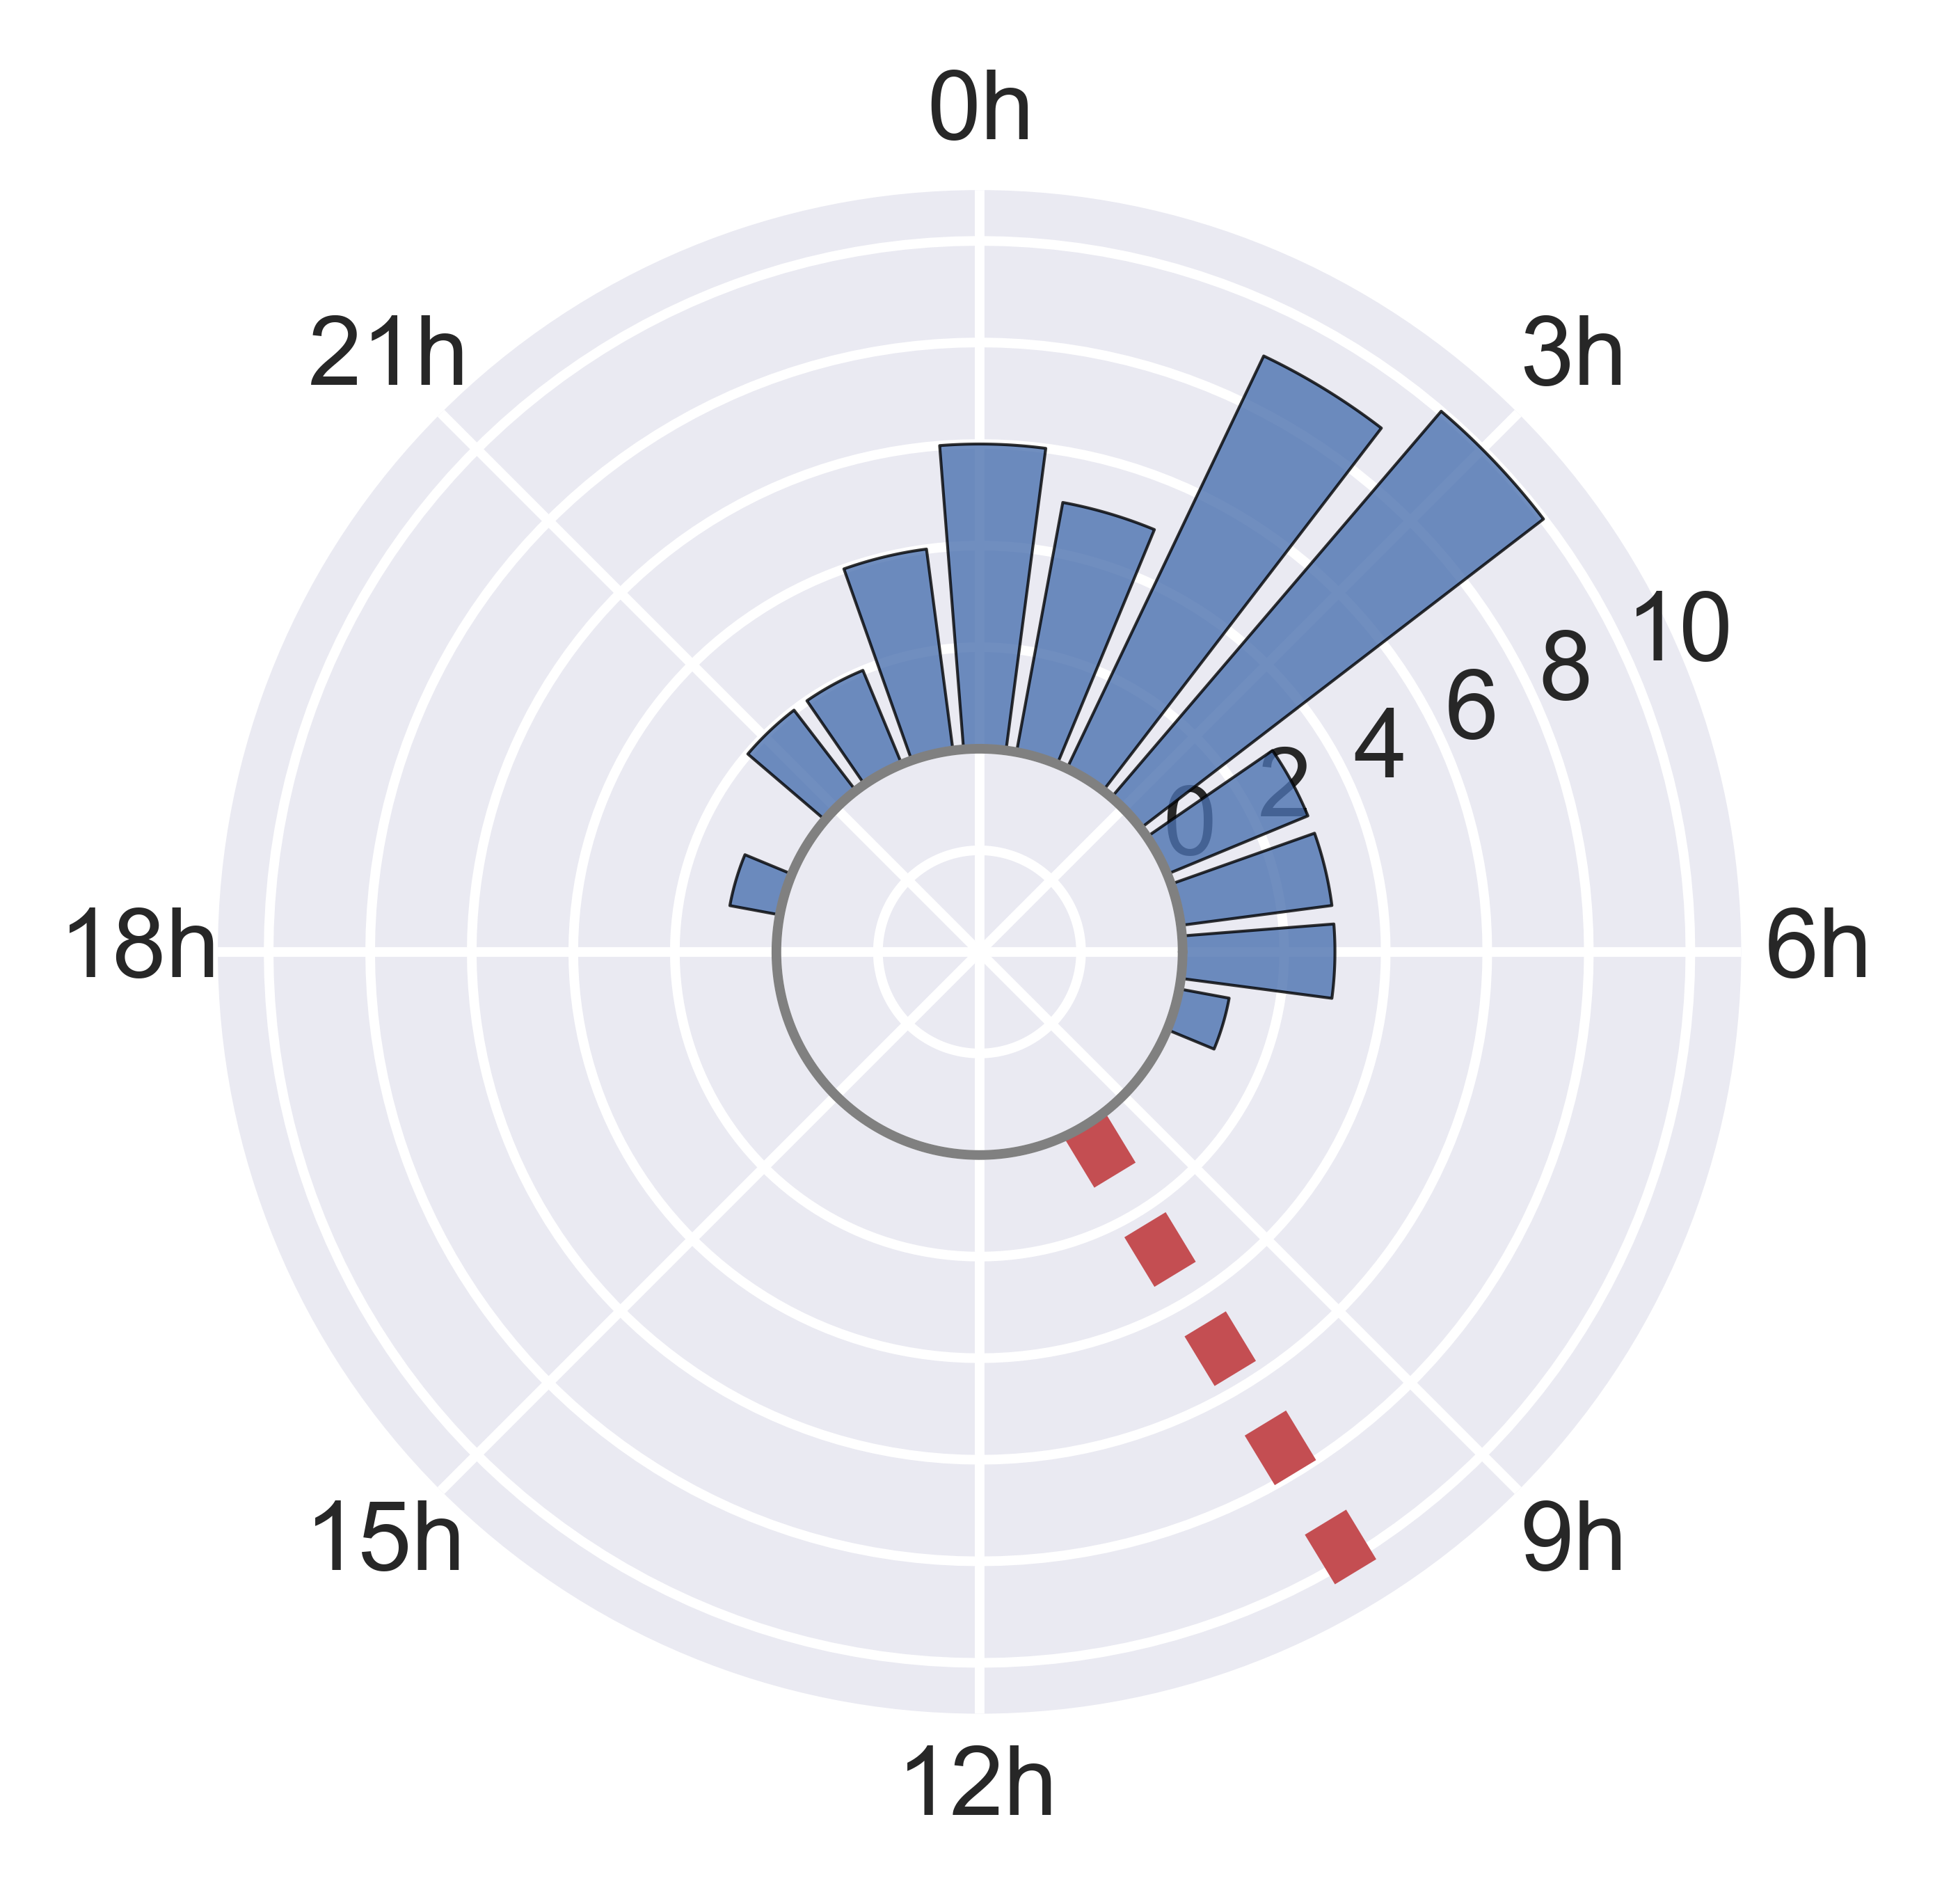
\includegraphics{ch4_fig_1c}
  \caption{Analysis of the time of a transaction using a 24 hour clock. The arithmetic mean of the 
  transactions time (dashed line) do not accurately represents the actual times distribution.}
  \label{fig:4:von1}
  \end{figure} 
  
  We propose to overcome this limitation by modeling the time of the transaction as a periodic 
  variable, in particular using the von Mises distribution \citep{Fisher1996}. The von Mises 
  distribution, also known   as the periodic normal distribution, is a distribution of a wrapped 
  normal distributed  variable across a circle. The von Mises probability distribution of a 
  set of examples $D=\{t_1,t_2,\cdots,t_N\}$ for a given angle $t_x$ is given by
  \begin{equation}
    f\left(t_x\vert \mu_{vM} , \sigma_{vM} \right) = \frac{e^{\frac{1}{\sigma_{vM}} \cos(t_x - 
\mu_{vM})}}{2 \pi I_0\left(\frac{1}{\sigma_{vM}}\right)}
  \end{equation}
%   \begin{equation}
%   D \sim vonmises\left( \mu_{vM} , \frac{1}{\sigma_{vM}} \right),
%   \end{equation}
  where  $I_0(\kappa)$ is the modified Bessel function of order 0, 
and   $\mu_{vM}$, $\sigma_{vM}$ are the periodic mean and periodic standard deviation, 
  respectively, and are defined as
  \begin{equation}
    \mu_{vM}(D) =  2\cdot \arctan\left(\frac{\phi}{\left(
    \sqrt{\psi^2 + \phi^2} +  \psi \right)} \right),
  \end{equation}
  and
  \begin{equation}
    \sigma_{vM}(D) = \sqrt{ ln\left( \frac{1}{
    \left(\frac{\phi}{N} \right)^2  + \left(\frac{\psi}{N} \right)^2 } \right) },
  \end{equation}
  respectively. Where $\phi=\sum_{t_j \in D} \sin(t_j)$ and $\psi=\sum_{t_j \in D }\cos(t_j)$ 
  \citep{Bishop2006}. 
  
  In particular we are interested in calculating a confidence interval ($CI$)   for the time of a 
  transaction. For doing that, initially we select a set of transactions made by  the same client 
  in the last $t_p$ hours,
  \begin{align}\label{eq:4:pe_features1}
    \mathcal{S}_{per} \equiv TRX_{vM}(\mathcal{S},i, t_p) & = \bigg\{ x_l^{time} \bigg\vert   
    \left(x_l^{id}=x_i^{id}\right)\wedge \nonumber \\
    &\left(hours(x_i^{time},x_l^{time})< t_p\right)    \bigg\}_{l=1}^N.
  \end{align}
  Afterwards, the probability distribution function of the time of the set of transactions is 
  calculated as:
  \begin{equation}
   x_i^{time} \sim vonmises\left(\mu_{vM}(\mathcal{S}_{per}), 
  \frac{1}{\sigma_{vM}(\mathcal{S}_{per})} \right).
  \end{equation}
  
  
  In \figurename{~\ref{fig:4:von2}}, the von Mises distribution calculation for the  earlier 
  example is shown. It is observed that the arithmetic mean is quite different from the periodic  
mean, the latter being a more realistic representation of the actual transactional times. Then, 
using the estimated distribution,   a new set of features can be extracted, ie., a binary  
  feature ($x_i^{p1}$) if a new transaction time is within the confidence interval range with 
  probability   $\alpha$. An example is presented in \figurename{~\ref{fig:4:von3}}. 
  Furthermore, other features can be calculated, as the confidence interval range can be calculated 
  for several values of $\alpha$, and also the time period can have an arbitrary size.

  \begin{figure}[!t]
  \centering
  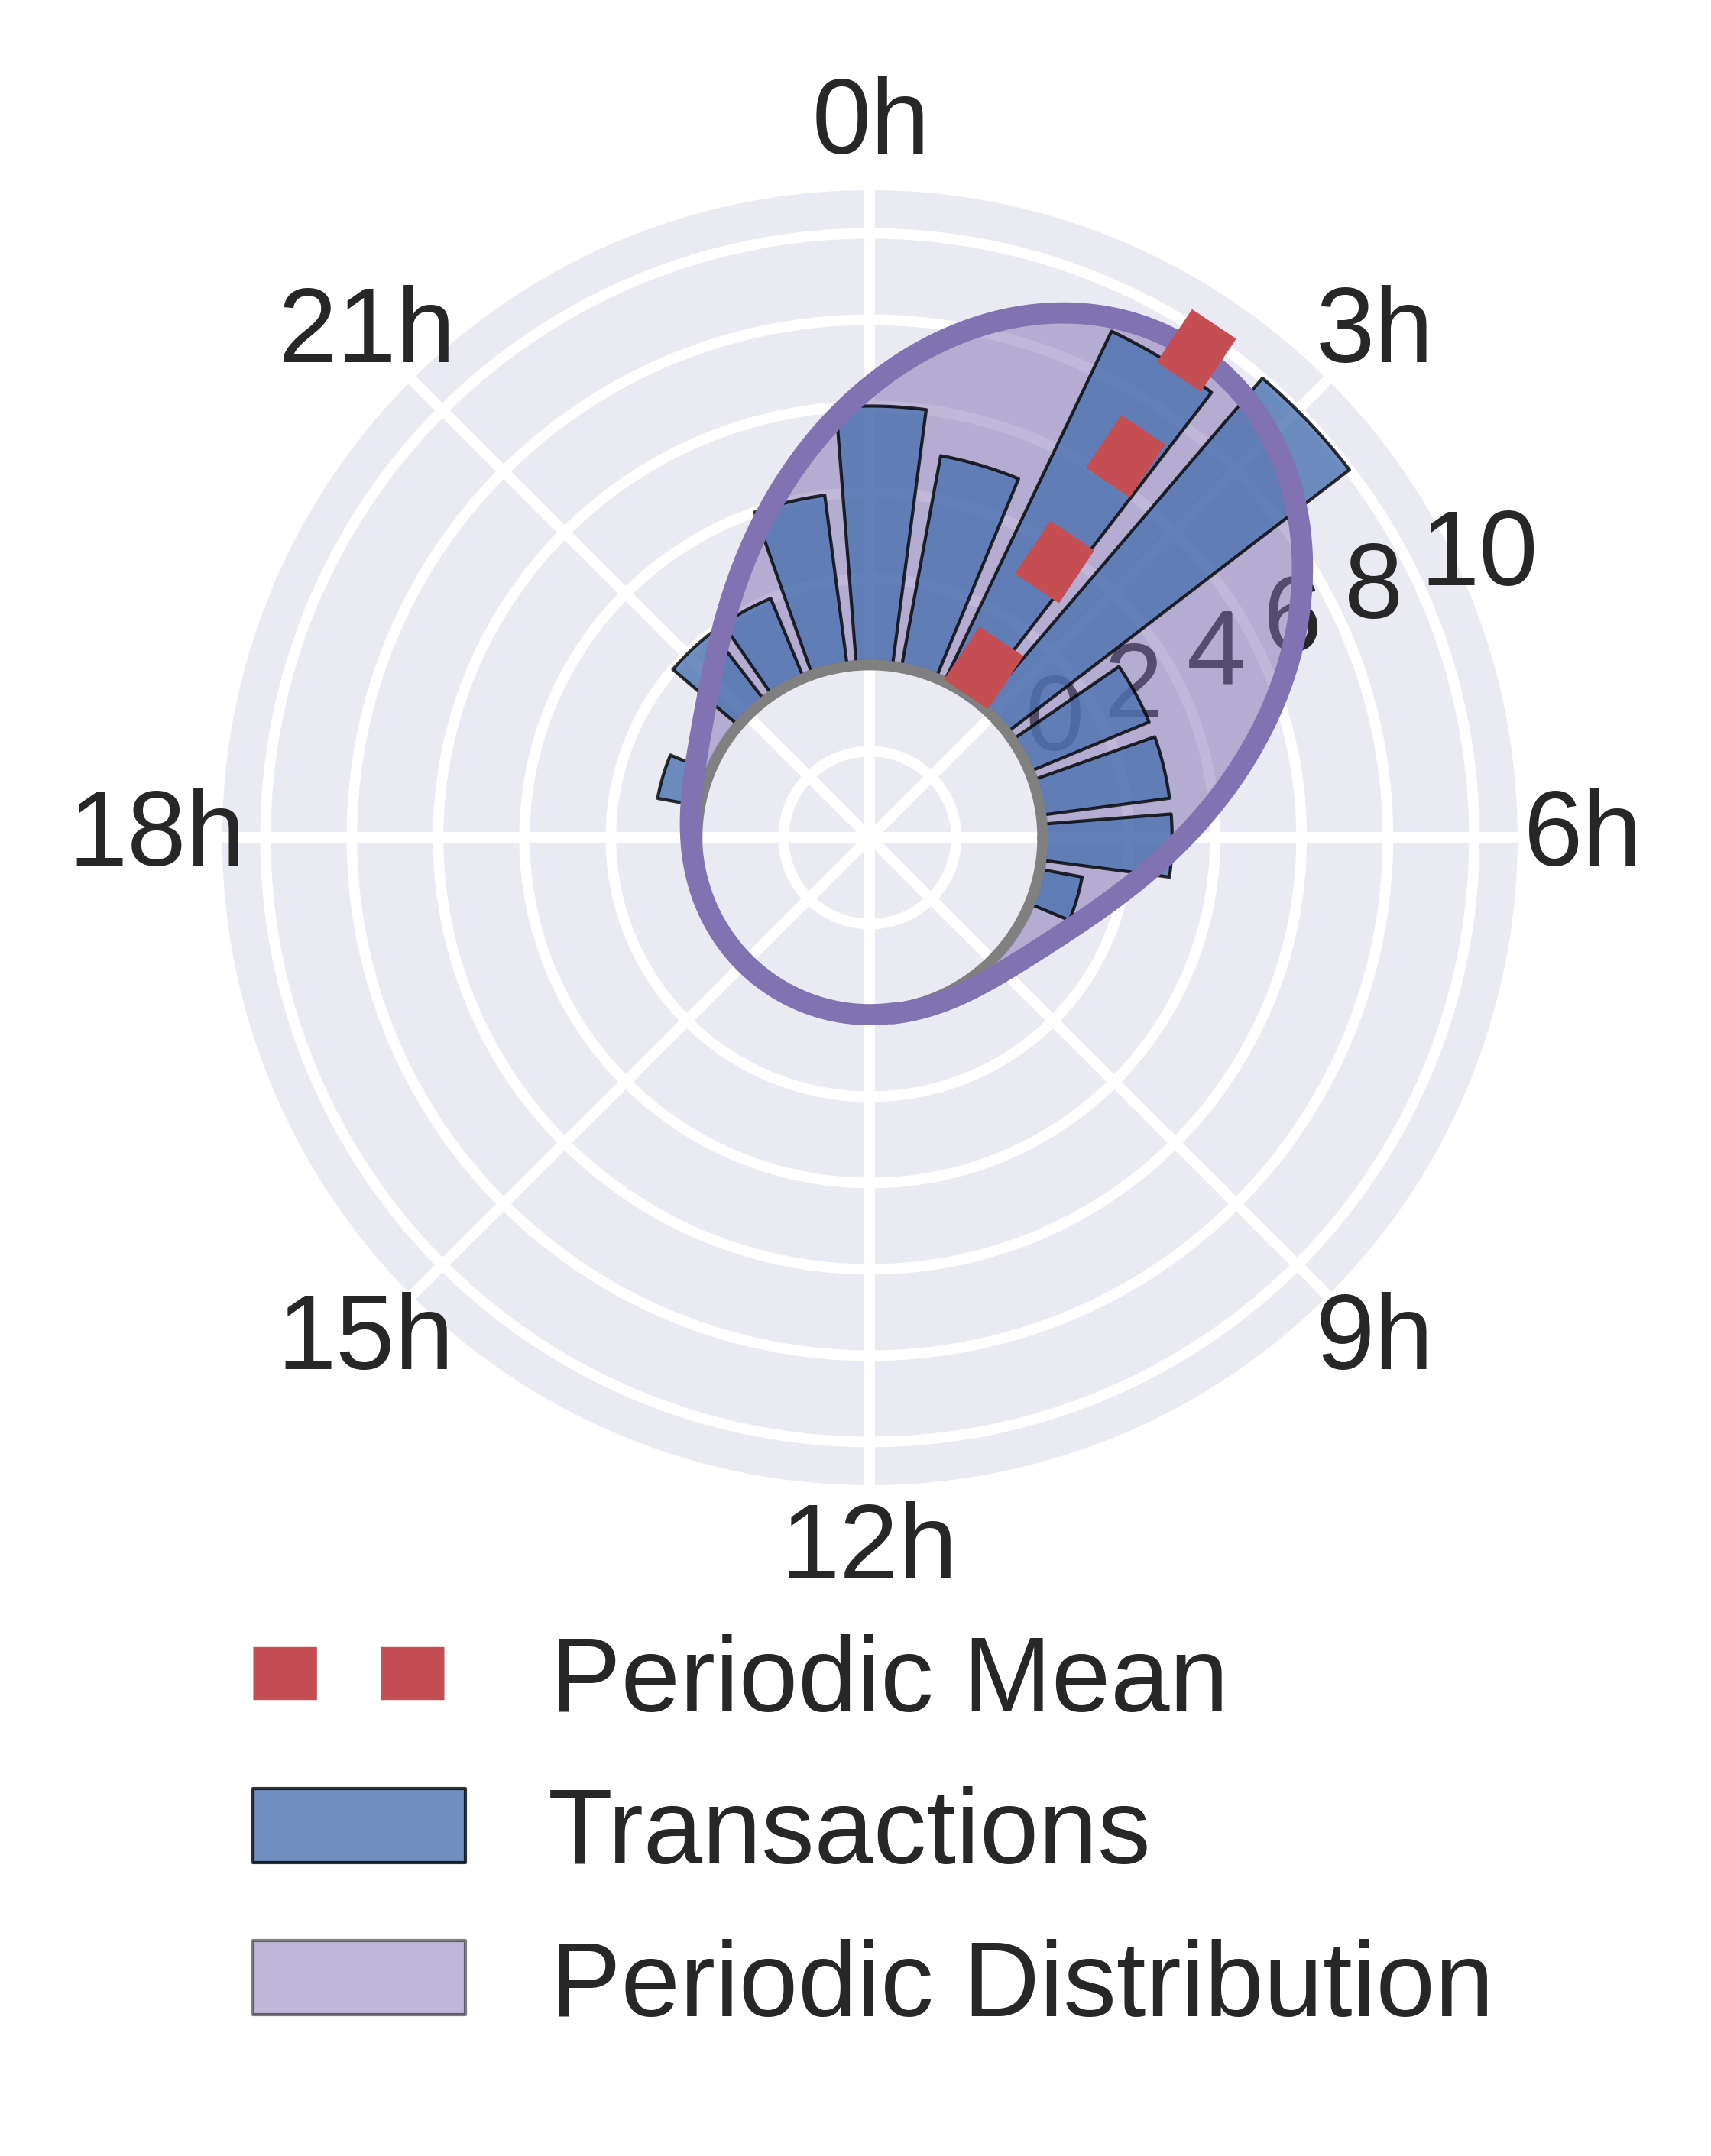
\includegraphics{ch4_fig_2c}
  \caption{Fitted von Mises distribution including the periodic mean (dashed line) and the 
    probability distribution (purple area).}
  \label{fig:4:von2}
  \end{figure} 
  
  \begin{figure}[!t]
  \centering
  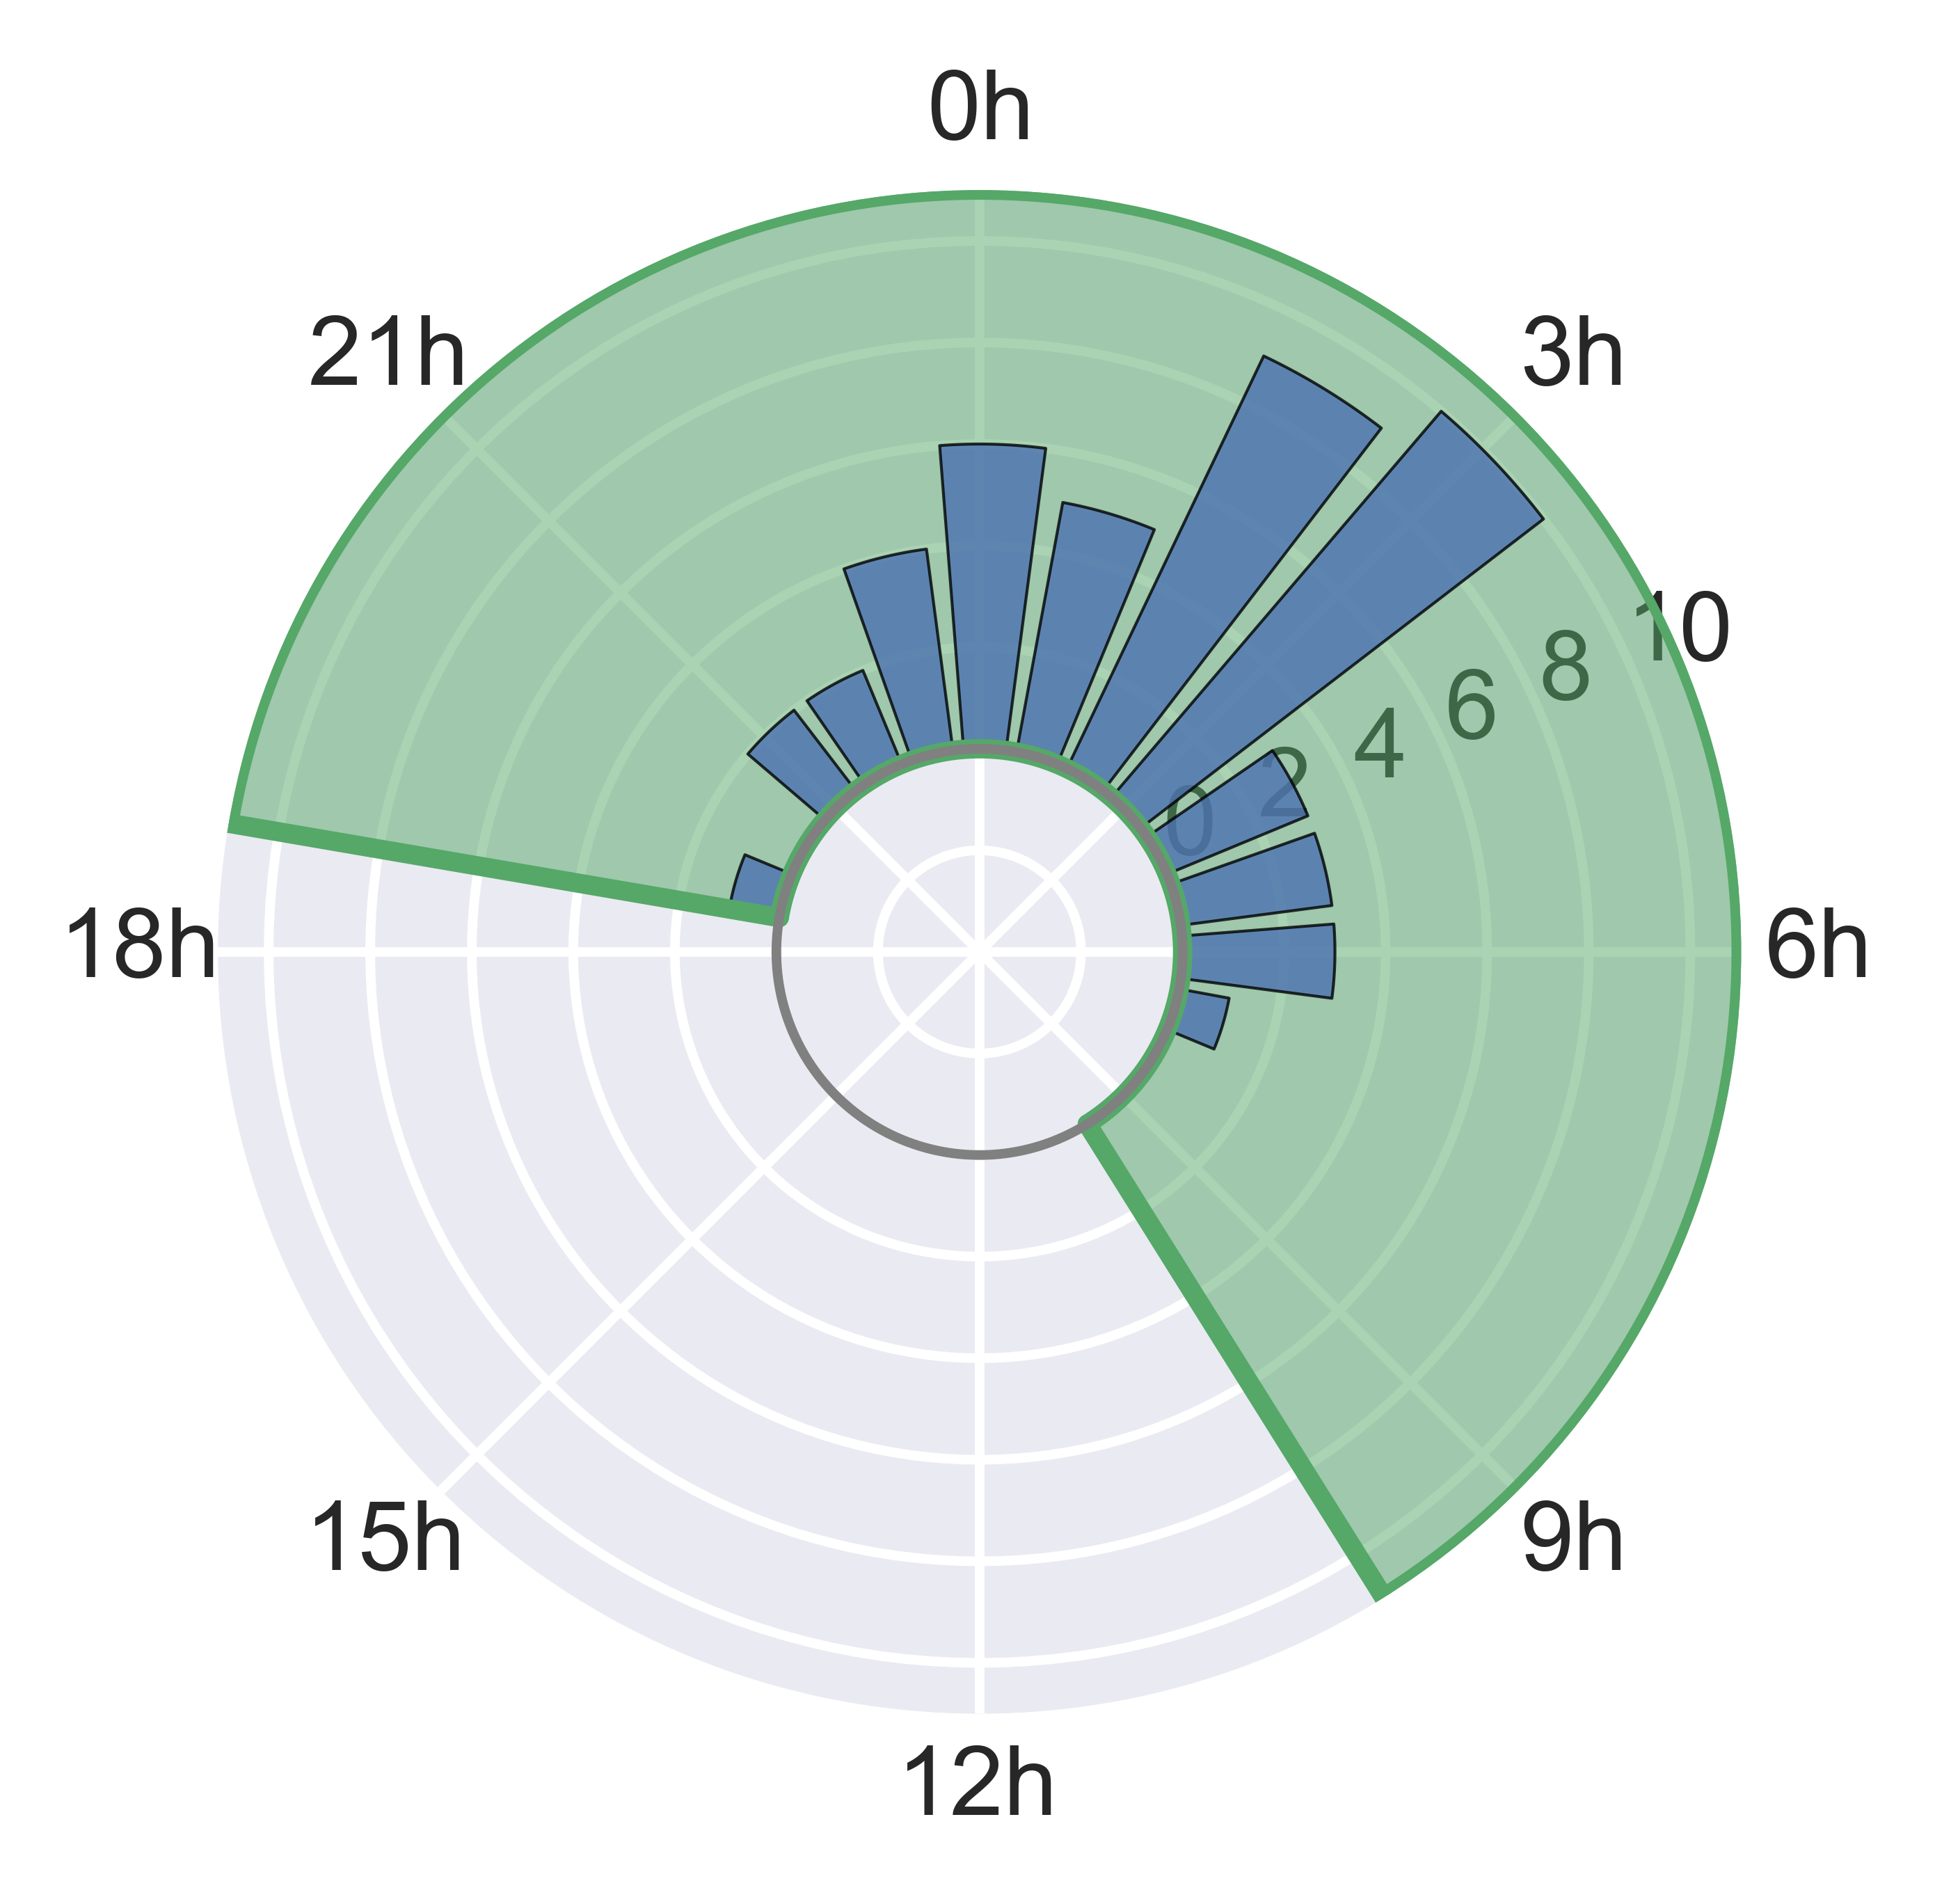
\includegraphics{ch4_fig_3c}
  \caption{Expected time of a transaction (green area). Using     the confidence interval, a  
  transaction can be flag normal   or   suspicious, depending     whether or  not the time of 
  the   transaction is within the   confidence  interval.}
  \label{fig:4:von3}
  \end{figure} 
	
Additionally, following the same example presented in 
\tablename{~\ref{tab:4:agg_features_example1}}, we calculate a feature $x_i^{p1}$, as a binary 
feature that takes the value of one if the current  time of the transaction is within the 
confidence interval of the time of the previous  transactions with a confidence of $\alpha=0.9$. 
The example is shown in \tablename{~\ref{tab:4:agg_features_example2}}, where the 
arithmetic and periodic   means differ, as for the last transaction both means are 
significantly different. Moreover, the  new feature helps to get a better understanding of 
when a customer is expected to make transactions.

	\begin{table}[!t]
   \centering
   \footnotesize
   \begin{tabular}{|c c | c | c c c|}
   \hline
   \multicolumn{2}{|c|}{\textbf{Raw features}} & \textbf{Arithmetic} & 
\multicolumn{3}{c|}{\textbf{Periodic features}} \\  \hline
   \textbf{Id} & \textbf{Time} & \textbf{mean} & \textbf{mean} & 
    \textbf{Confidence interval} & $x_i^{p1}$ \\
   \hline
		1& 01/01 18:20& --- & ---	 &	--- & ---\\
		2& 01/01 20:45& --- & ---	 &---	 & ---\\
		3& 01/01 22:40& 19:27 & 19:27 & 15:45 - 23:10 & True \\
		4& 02/01 00:50& 20:28 & 20:28 & 17:54 - 23:03 & False\\
		5& 02/01 19:18& 16:44 & 22:44 & 18:51 - 00:17 & True\\
		6& 02/01 23:45& 16:19 & 21:07 & 15:21 - 02:52 & True\\
		7& 03/01 06:00& 18:43 & 22:43 & 17:19 - 01:46 & False\\
   \hline
   \end{tabular}
   \caption{Example calculation of periodic features.}
   \label{tab:4:agg_features_example2}
   \end{table}
  
  Finally, when calculating the periodic features, it is important to use longer time frames $t_p$, 
  since if the distribution is calculated using only a couple of transactions it may not be as 
  relevant of a customer behavior patterns, compared against using a full year of transactions.
  Evidently, if $t_c$ is less than 24 hours, any transaction made afterwards will not be expected 
  to be within the distribution of previous transactional times. To avoid this, we recommend using 
  at least the previous 7 days of transactional information, therefore, having a better 
  understanding  of its behavioral patterns. Lastly, this approach can also be used to estimate 
  features such as  the expected day of the week  of transactions, as some customers may only use 
  their credit cards  during the weekend nights, or during working hours.
	
	\subsection{Database}

 	For this thesis we use a dataset provided by a large European card processing company. The 
	dataset consists of fraudulent and legitimate transactions made with credit and debit cards 
	between January 2012 and June 2013. The total dataset contains 120,000,000 individual 
	transactions, each one with 27 attributes, including a fraud label indicating whenever a 
	transaction is identified as fraud. This label was created internally in the card processing 
	company, and can be regarded as highly accurate. In the dataset only 40,000 transactions were 
	labeled as fraud, leading to a fraud ratio of 0.025\%. 

	
\section{Credit scoring}
\label{sec:4:creditscoring}

  In this section, we consider the second financial risk management application, namely, credit 
  scoring.
  In order to mitigate the impact of credit risk and make more objective and accurate decisions, 
  financial institutions use credit scores to predict and control their losses.
  The objective in credit scoring is to classify which potential customers are likely to default a 
  contracted financial obligation based on the customer's past financial experience, and with that 
  information decide whether to approve or decline a loan~\citep{Anderson2007}. This tool has 
  become a standard practice among financial institutions around the world in order to predict 
  and control their loans portfolios. When constructing credit scores, it is a common practice to 
  use standard cost-insensitive binary classification algorithms such as logistic regression, 
  neural networks, discriminant analysis, genetic programing, decision trees, among 
  others~\citep{Hand1997,Bahnsen2011}. 
  
  Formally, a credit score is a statistical model that allows the estimation of the probability 
  $\hat p_i=P(y_i=1|\mathbf{x}_i)$ of a customer $i$ defaulting a contracted debt. Additionally, 
since the 
  objective of credit scoring is to estimate a classifier $c_i$ to decide whether or not to grant a 
  loan to a customer $i$, a threshold $t$ is defined such that if $\hat p_i <t$, then the loan is 
  granted, i.e., $c_i(t)=0$, and denied otherwise, i.e., $c_i(t)=1$.
  
  There exists different approaches for defining the probability threshold. The sensitivity versus 
  specificity ($SvsS$) approach is the most widely used among financial institutions 
  \citep{Anderson2007}, where specificity is the true positive rate $F_0(t)$ for a threshold $t$, 
  and the sensitivity is one minus the false positive rate $F_1(t)$ given a threshold $t$ 
  \citep{Hernandez-Orallo2012}. In this method the objective is to fix the threshold at the point 
  where the sensitivity is equal to the specificity $F_0(t)=1-F_1(t)$, where $F_0(t)$ and $F_1(t)$ 
  are calculated using:
  \begin{equation}
   F_a(t)=\frac{1}{N_a}\vert \{ \mathbf{x}_i \vert \mathbf{x}_i \in \mathcal{S}_a \wedge \hat p_i 
  \le t \}\vert, \text{ for }  a\in\{0,1\}.
  \end{equation}
  Lastly, the $SvsS$ threshold $t_{SvsS}$ is found by using
  \begin{equation}
  t_{SvsS}= \argmin_t \vert F_0(t) - (1-F_1(t)) \vert.
  \end{equation}
  This process is further clarified in \figurename{ \ref{fig:ch4:4}}.
  
  \begin{figure}
  \centering
  \centering
  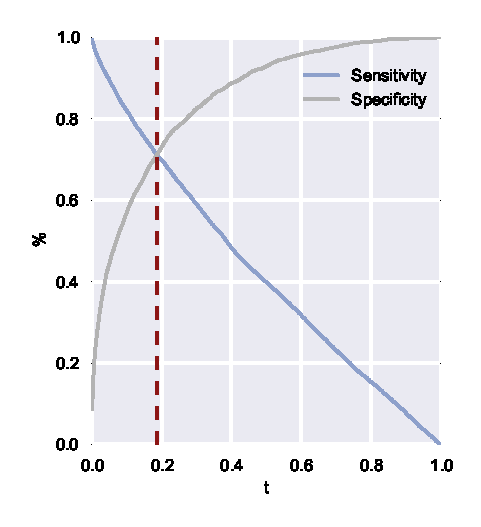
\includegraphics{ch4_fig_4}
  \caption{Credit scoring sensitivity versus specificity thresholding procedure.}
  \label{fig:ch4:4}
  \end{figure}
  
  After the classifier $c_i$ is estimated, there is a need to evaluate its performance. In 
  practice, many statistical evaluation measures are used to assess the performance of a credit 
  scoring model. Measures such as the area under the  receiver operating characteristic curve (AUC),
  Brier score, Kolmogorov-Smirnoff (K-S) statistic,  $F_1$-Score, and misclassification are among 
  the most common \citep{Beling2005}. Nevertheless, none of these measures takes into account the 
  business and economical realities that take place in credit scoring. Costs that the financial 
  institution had incurred to acquire customers, or the expected profit due to a particular client, 
  are not considered in the evaluation of the different models. This is explored in detail in the 
  next section.

  
  \subsection{Financial evaluation of a credit scorecard }
  
  Typically, a credit risk model is evaluated using standard cost-insensitive measures.
  However, in practice, the cost associated with approving 
  what is known as a bad customer, i.e., a customer who defaulted his credit loan, is quite 
  different from the cost associated with declining a good customer,  i.e., a customer who 
  successfully repaid his credit loan. Furthermore, the costs are not constant among customers. 
  This is because loans have different credit line amounts, terms, and even interest rates. Some 
  authors have proposed methods that include the misclassification costs in the credit scoring 
  context \citep{Verbraken2014,Alejo2013,Beling2005,Oliver2009}. However, they assume a constant 
  misclassification cost, which is not the case in credit scoring.
  
 
  Initial approaches to include the different costs have been published in recent years, 
  particularly the one proposed by Beling et al. \citep{Beling2005,Oliver2009}, in which the costs 
  of misclassification are assigned for each error. Specifically, setting the cost of a false 
  positive $C_{FP}$ to the loan's annual interest rate charged to the customer $int_r$, the cost of 
  a false negative $C_{FN}$ to the loss given default $L_{gd}$, which is the percentage of loss 
  over the total credit line when the customer defaulted, and setting to zero the costs of true 
  positive $C_{TP}$ and true negative $C_{TN}$. Using that, they proposed the expected cost (EC) 
  method to find the probability threshold that minimizes those costs, $t_{ec}= 
  \frac{C_{FN}}{C_{FN}+C_{FP}} =\frac{L_{gd}}{L_{gd}+int_r}.$ Nevertheless, this approach assumes 
  a constant cost within examples, which is a strong assumption, since in practice each example 
  carries a very different cost given by the different credit limits and conditions of each loan. 
  Consequently, there is a need for an example-dependent cost matrix that takes into account the 
  cost of misclassifying each example.
  
  
  \subsubsection{Example-dependent cost-sensitive evaluation measure}
  
  In order to take into account the varying costs that each example carries, we propose 
  a cost matrix with example-dependent misclassification costs as 
  given in \tablename{~\ref{tab:4:costmat2}}. First, we assume that the costs of a correct 
  classification, $C_{TP_i}$ and $C_{TN_i}$, are zero for every customer $i$. We define $C_{FN_i}$ 
   the losses if the customer $i$ defaults to be proportional to his credit line $Cl_i$. We 
  define the cost of a false positive per customer $C_{FP_i}$ as the sum of two real financial 
  costs $r_i$ and $C^a_{FP}$, where $r_i$ is the loss in profit by rejecting what would have been a 
  good customer. 
  
  \begin{table}
  \centering
  \footnotesize
    \begin{tabular}{c|c|c}
    %\cline{2-3}
      \multicolumn{1}{c|}{}  & Actual Positive& Actual Negative \\
      \multicolumn{1}{c|}{} & $y_i=1$& $y_i=0$ \\
      \hline
      Predicted Positive& \multirow{ 2}{*}{$C_{TP_i}=0$} & \multirow{2}{*}{$C_{FP_i}=r_i+C^a_{FP}$} 
      \\
      $c_i=1$ & &\\
      \hline
      Predicted Negative& \multirow{ 2}{*}{$C_{FN_i}=Cl_i \cdot L_{gd}$} & \multirow{
      2}{*}{$C_{TN_i}=0$} \\
      $c_i=0$ & &\\
    \end{tabular}
  \caption{Credit scoring example-dependent cost matrix}
  \label{tab:4:costmat2}
  \end{table}
  
  The profit per customer $r_i$ is calculated as the present value of the difference between the 
  financial institution gains and expenses, given the credit line $Cl_i$, the term $l_i$ and the 
  financial institution lending rate $int_{r_i}$ for customer $i$, and the financial institution 
  of cost funds $int_{cf}$.
  \begin{equation}
    r_i= PV(A(Cl_i,int_{r_i},l_i),int_{cf},l_i)-Cl_i,
  \end{equation}
  with $A$ being the customer monthly payment and $PV$ the present value of the monthly payments,
  which are calculated using the time value of money equations \citep{Lawrence2012},
  \begin{eqnarray}
    A(Cl_i,int_{r_i},l_i) &=&  Cl_i \frac{int_{r_i}(1+int_{r_i})^{l_i}}{(1+int_{r_i})^{l_i}-1},
  \end{eqnarray}
  and 
  \begin{eqnarray}
    PV(A,int_{cf},l_i) &=& \frac{A}{int_{cf}} \left(1-\frac{1}{(1+int_{cf})^{l_i}} \right).
  \end{eqnarray}
    
  The second term $C^a_{FP}$ is related to the assumption that the financial institution will not 
  keep the money of the declined customer idle. It will instead give a loan to an alternative 
  customer \citep{Nayak1997}. Since no further information is known about the alternative customer, 
  it is assumed to have an average credit line $\overline{Cl}$ and an average profit $\overline{r}$.
  Given that, the false positive cost for an alternative customer becomes 
  \begin{equation}
    C^a_{FP}=- \overline{r} \cdot \pi_0+\overline{Cl}\cdot L_{gd} \cdot \pi_1,
  \end{equation}
  in other words minus the profit of an average alternative customer plus the expected loss, 
  taking into account that the alternative customer will pay his debt with a probability equal to 
  the prior negative rate, and similarly will default with probability equal to the prior positive 
  rate.

  \subsubsection{Calculation of the credit limit}
  
  One key parameter of our model is the credit limit. There exists several strategies to calculate 
  the $Cl_i$ depending on the type of loans, the state of the economy, the current portfolio, 
  among others \citep{Anderson2007,Lawrence2012}. Nevertheless, given the lack of information 
  regarding the specific business environments of the considered datasets, we simply define 
  $Cl_i$ as
  \begin{equation}\label{eq:cli}
      Cl_i = \min \bigg\{ q \cdot Inc_i, Cl_{max}, Cl_{max}(debt_i) \bigg\},
  \end{equation}
  where $Inc_i$ and $debt_i$ are the monthly income and debt ratio of the customer $i$, 
  respectively, $q$ is a parameter that defines the maximum $Cl_i$ as a function of the $Inc_i$, 
  and  $Cl_{max}$ the maximum overall credit line. Lastly, the maximum credit line given the 
  current debt is calculated as the maximum credit limit such that the current debt ratio plus the 
  new  monthly payment does not surpass the customer monthly income. It is calculated as
  \begin{equation}
    Cl_{max}(debt_i)=PV\left(Inc_i \cdot P_{m}(debt_i),int_{r_i},l_i\right),
  \end{equation}
  and
  \begin{equation}
    P_{m}(debt_i)=\min \left\{ \frac{A(q \cdot Inc_i,int_{r_i},l_i)}{Inc_i},\left(1-debt_i 
    \right) \right\}.
  \end{equation}
  
  
  \subsection{Databases}

    For this thesis we use two different publicly available credit scoring datasets. The first 
    dataset is the \textbf{2011 Kaggle competition Give Me Some Credit}\footnote{ 
    http://www.kaggle.com/c/GiveMeSomeCredit/}, in which the objective is to identify those 
    customers of personal loans that will experience financial distress in the next two years.
    The second dataset is from the \textbf{2009 Pacific-Asia Knowledge Discovery and Data Mining 
    conference (PAKDD) competition}\footnote{http://sede.neurotech.com.br:443/PAKDD2009/}.
    Similarly, this competition had the objective of identifying which credit card applicants
    were likely to default and by doing so deciding whether or not to approve their applications.
    The Kaggle Credit and PAKDD Credit datasets contain information regarding the features, and 
    more importantly about the income of each example, from which an estimated credit limit 
    $Cl_i$ can be calculated.
    
    The Kaggle Credit dataset contains 112,915 examples, each one with 10 features and the class 
    label. The proportion of default or positive examples is 6.74\%. 
    On the other hand, the PAKDD Credit dataset contains 38,969 examples, with 30 features and the 
    class label, with a proportion of 19.88\% positives. This database comes from a Brazilian 
    financial institution, and as it can be inferred from the competition description, the data 
    was obtained around 2004.
   
   
\begin{table}
\centering
\footnotesize
\begin{tabular}{lcc}
\hline
\multirow{ 2}{*}{Parameter}&Kaggle& PAKDD \\
  & Credit& Credit \\
  \hline
  Interest rate ($int_r$) &  4.79\% & 63.0\% \\
  Cost of funds ($int_{cf}$) & 2.94\% & 16.5\% \\
  Term ($l$) in months & 24 & 24 \\
  Loss given default ($L_{gd}$) &75\% & 75\% \\
  Times income ($q$) & 3 & 3 \\
  Maximum credit line ($Cl_{max}$) & 25,000 & 25,000\\
  \hline
\end{tabular}
\caption{Credit scoring model parameters}
\label{tab:4:parameters}
\end{table}

    Since no specific information regarding the datasets is provided, we assume that they belong to 
    average European and Brazilian financial institutions. This enable us to find the different 
    parameters needed to calculate the cost measure. In Table~\ref{tab:4:parameters}, the different 
    parameters are shown. In particular, we obtained the average interest rates in Europe during 
    2013 from the European Central Bank \citep{ECB2014}, and the average interest and exchange 
    rates in Brazil during 2004 from Trading Economics \citep{Economics2014}. Because the income 
    is not in the same currency on both datasets, we convert the PAKDD Credit dataset to Euros.
    Additionally, we use a fixed loan term $l$ for both datasets, considering that in the Kaggle 
    Credit dataset the class was constructed to predict two years of credit behavior, and 
    because the PAKDD Credit dataset is related to credit cards the term is fixed to two years 
    \citep{Lawrence2012}. Moreover, we set the loss given default $L_{gd}$ using information from 
    the Basel II standard\footnote{http://www.bis.org/publ/bcbsca.htm.}, $q$ to 3 since it is the 
    average personal loan requests related to monthly income, and the maximum credit limit 
    $Cl_{max}$ to 25,000 Euros.

    
\section{Summary of the datasets}

For each dataset we used a pre-define cost matrix as shown in Section~\ref{sec:4:fraud} and 
Section~\ref{sec:4:creditscoring}. Additionally,  for each database, 3 different 
datasets are extracted: training, validation and testing. Each one containing 50\%, 25\% and 25\% of 
the examples, respectively. Afterwards, because classification algorithms suffer when the label 
distribution is skewed towards one of the classes \citep{Hastie2009}, an under-sampling of the 
positive examples is made, in order to have a balanced class distribution. Moreover, we perform the 
cost-proportionate rejection-sampling and cost proportionate over-sampling procedures, that we 
previously described in Section~\ref{sec:3:costsampling}. \tablename{~\ref{tab:4:databases}}, 
summarizes the different datasets. It is important to note that the sampling procedures were only 
applied to the training dataset since the validation and test datasets must reflect the real 
distribution.

\begin{table}[ht!]
  \centering
  \footnotesize
  \begin{tabular}{l l c c c } %sum 7.7
    \hline
    \textbf{Database}& \textbf{Set}&  $N$ & $\pi_1$ & Cost (Euros) \\
    \hline
    Fraud &Total&236,735&1.50&895,154\\
    Detection&  Training ($t$)&94,599&1.51&358,078\\
    &Under-sampled ($u$)&2,828&50.42&358,078\\
    &Rejection-sampled ($r$)&94,522&1.43&357,927\\
    &Over-sampled ($o$)&189,115&1.46&716,006\\
    &Validation&70,910&1.53&274,910\\
    &Testing&71,226&1.45&262,167\\
    \hline
    Credit  & Total&112,915&6.74&83,740,181\\
    Scoring 1 & Training ($t$)&45,264&6.75&33,360,130\\
    &Under-sampled ($u$)&6,038&50.58&33,360,130\\
    &Rejection-sampled ($r$)&5,271&43.81&29,009,564\\
    &Over-sampled ($o$)&66,123&36.16&296,515,655\\
    &Validation&33,919&6.68&24,786,997\\
    &Testing&33,732&6.81&25,593,055\\
    \hline
    Credit &Total&38,969&19.88&3,117,960\\
    Scoring 2&Training ($t$)&15,353&19.97&1,221,174\\
    &Under-sampled ($u$)&6,188&49.56&1,221,174\\
    &Rejection-sampled ($r$)&2,776&35.77&631,595\\
    &Over-sampled ($o$)&33,805&33.93&6,798,282\\
    &Validation&11,833&20.36&991,795\\
    &Testing&11,783&19.30&904,991\\
    \hline
  \end{tabular}
  \caption{Summary of the datasets. Where $N$ is the number of examples and $\pi_1$ is the 
  percentage of positives examples.}
  \label{tab:4:databases}
\end{table}

\makeatletter
\setlength{\@fptop}{0pt}
\makeatother\cleardoublepage
	\chapter{Marketing Analytics}\label{ch:5}

\begin{remark}{Outline}
In this chapter, we present two different marketing real-world example-dependent 
cost-sensitive problems, namely, churn modeling and direct marketing. Both problems deal 
with identifying those customers with certain characteristic with the objective to maximize the 
results of the different CRM strategies.
First, we introduce the churn modeling problem and present the propose financial evaluation 
measure for a churn campaign in Section \ref{sec:5:churn}. Lastly in Section 
\ref{sec:5:directmarketing}, the direct marketing problem is presented including the propose 
example-dependent cost-sensitive cost matrix for evaluating this problem.
\end{remark}


\section{Churn modeling}
\label{sec:5:churn}

Customer churn predictive modeling deals with predicting the probability of a customer defecting 
using historical, behavioral and socio-economical information. This tool is of great benefit to 
subscription based companies allowing them to maximize the results of retention campaigns. The 
problem of churn predictive modeling has been widely studied by the data mining and machine learning
communities. It is usually tackled by using classification algorithms in order to learn the 
different patterns of both the churners and non-churners. Nevertheless, current state-of-the-art 
classification algorithms are not well aligned with commercial goals, in the sense that, the models 
miss to include the real financial costs and benefits during the training and evaluation phases. In 
the case of churn, evaluating a model based on a traditional measure such as accuracy or predictive 
power, does not yield to the best results when measured by the actual financial cost, i.e., 
investment per subscriber on a loyalty campaign and the financial impact of failing to detect a 
real churner versus wrongly predicting a non-churner as a churner.

In this section, we propose a cost-sensitive framework for customer churn predictive 
modeling. First, in Section \ref{sec:5:1:intro}, we introduce 
the problem of chrun modeling. Then in Section \ref{sec:5:1:evaluation}, we present a financial 
based measure for evaluating the effectiveness of a churn campaign taking into account the 
available 
portfolio of offers, their individual financial cost and probability of offer acceptance depending 
on the customer profile. Finally, in Section~\ref{sec:5:1:data}, we describe the real-world churn 
modeling dataset that will be used during the experiments.


\subsection{Flow analysis of a churn campaign}
\label{sec:5:1:intro}

The two main objectives of subscription-based companies are to  acquire new subscribers and 
retain those they already have, mainly because profits are directly linked with the number of 
subscribers.  In order to maximize the profit, companies must increase the customer base by 
incrementing sales  while decreasing the number of churners. Furthermore, it is common knowledge 
that retaining a  customer is about five times less expensive than acquiring a new one 
\citep{Farris2010}, this creates  pressure to have better and more effective churn campaigns.

A typical churn campaign consists in identifying from the current customer base which ones are 
more likely to leave the company, and make an offer in order to avoid that behavior.
With this in mind the companies use intelligence to create and improve retention and collection
strategies. In the first case, this usually implies an offer that can be either a discount or a 
free upgrade during certain span of time. In both cases the company has to 	assume a cost for that 
offer, therefore, accurate prediction of the churners becomes important. The logic of this flow is 
shown in \figurename{ \ref{fig:ch5:1}}.

The churn campaign process starts with the sales that every month increase the customer 
base, however, monthly there is a group of customers that decide to leave the company for many 
reasons. Then the objective of a churn model is to identify those customers before they take the 
decision of defecting.

Using a churn model, those customers more likely to leave are predicted as churners and 
an offer is made in order to retain them. However, it is known that not all customers will accept 
the offer, in the case when a customer is planning to defect, it is possible that the offer is not 
good enough to retain him or that the reason for defecting can not be influenced by an offer.
Using historical information, it is estimated that a customer will accept the offer with 
probability $\gamma$.
On the other hand, there is the case in which the churn model misclassified a non-churner as 
churner, also known as false positives, in that case the customer will always accept the offer that 
means and additional cost to the company since those misclassified customers do not have the 
intentions of leaving.

  \begin{figure}[t]
    \centering
    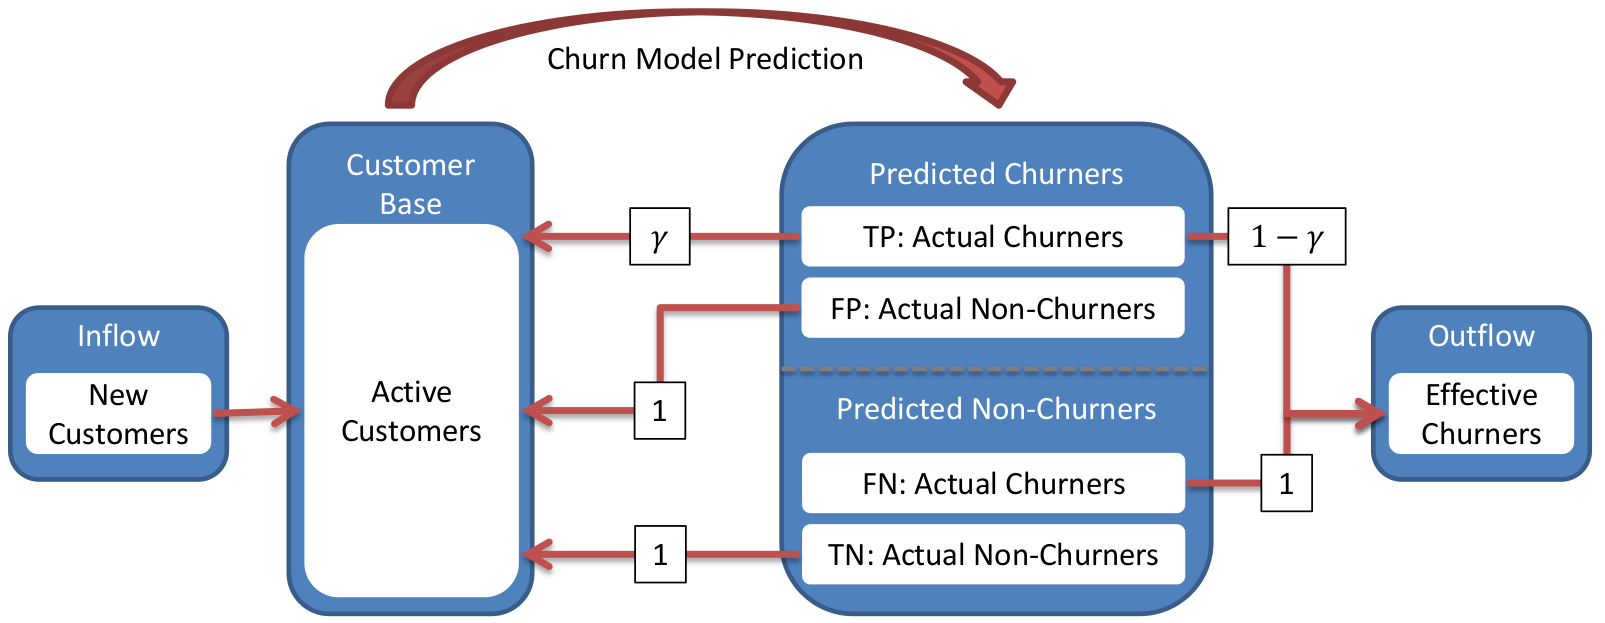
\includegraphics[width=11.5cm]{ch5_fig1}   %CHANGE TO 12cm
    \caption{Flow analysis of a churn campaign \citep{Verbraken2012}}
    \label{fig:ch5:1}
  \end{figure}
  
In the case were the churn model predicts customers as non-churners, there is also the possibility 
of a misclassification, in this case an actual churner is predicted as non-churner, since 
these customers do not receive an offer and they will leave the company, these cases are known as 
false negatives. Lastly, there is the case were the customers are actually non-churners, then 
there is no need to make a retention offer to these customers since they will continue to be part 
of the customer base.

It can be seen that a churn campaign (or churn model) has three main points. First, avoid false 
positives since there is a financial cost of making an offer where it is not needed. Second, find 
the right offer to give to those customers identified as churners. And lastly, to decrease 
the number of false negatives.

From a machine learning perspective, a churn model is a classification algorithm.
In the sense that using historical information, a prediction of which current customers 
are more likely to defect, is made. This model is normally created using one of a number of 
well established algorithms (Logistic regression, neural networks, random forests, among 
others) \citep{Ngai2009,KhakAbi2010}. Then, the model is evaluated using measures such as 
misclassification error, receiver operating characteristic ($ROC$),  Kolmogorov-Smirnov ($KS$) 
or \mbox{$F_1Score$} statistics \citep{Verbeke2012}. 
However, these measures may not be the most appropriate evaluation criteria when  
evaluating a churn model, because they tacitly assume that misclassification errors carry the 
same cost, similarly with the correct classified examples. This assumption does not hold in many 
real-world applications such as churn modeling, since  when misidentifying a churner the financial 
losses are quite different than when misclassifying a non-churner as churner \citep{Glady2009}. 
Furthermore, the accuracy measure also assumes that the class distribution 
among examples is constant and balanced \citep{Provost1998}, and typically the distributions of a 
churn data set are skewed \citep{Verbeke2012}.
	
In the next section, we propose a new financial based measure for evaluating the effectiveness of 
a voluntary churn campaign taking into account the available portfolio of offers, their 
individual 	financial cost and probability of acceptance depending on the customer profile. 


\subsection{Propose evaluation measure of a churn campaign}
\label{sec:5:1:evaluation}
	
Different studies have proposed measures to deal with these cost-sensitivity related to
evaluating a churn model. In \citep{Neslin2006}, a profit-based measure was proposed by starting 
with the confusion matrix and multiplying it with the expected profit of each case.

\begin{align}\label{eq:5:profit1}
 Profit_1 = (TP+FP)\bigg[ & \left(\gamma CLV + C_o(1-\gamma)(-C_a)\right)\pi_1\gamma \nonumber \\
 & -C_o-C_a\bigg]-N\cdot C_a,
\end{align}
with $C_a$ being the fixed administrative cost of running the campaign, $C_o$ the average 
cost of the retention offer, $C_a$ the cost of contacting the customer, $\pi_1$ the prior churn rate 
and $CLV$ the average customer lifetime value or the present value of the expected profit that a 
customer will generate. Moreover, as discussed in \citep{Verbraken2013}, if the average instead of 
the total profit is considered and the fixed cost $N\cdot C_a$ is discarded since it is irrelevant 
for the classifier selection, the profit can be expressed as:
\begin{align}\label{eq:5:profit2}
 Profit_2 = &TP\left(\gamma(CLV-C_o-C_a)+(1-\gamma)C_a \right) \nonumber \\
 &+FP(-C_o-C_a).
\end{align}

Nevertheless, equations (\ref{eq:5:profit1}) and (\ref{eq:5:profit2}) assume that every customer 
has the same $CLV$ and $C_o$, whereas this is not true in practice. In fact, different customers 
have a very different $CLV$, and not all offers can be made to every customer, neither do they have 
the same impact across customers. In order to obtain a more business oriented measure, we first 
analyze the financial impact of the different decisions, i.e., false positives, false negatives, 
true positives and true negatives, for each customer.	

\begin{figure}[t]
  \centering
  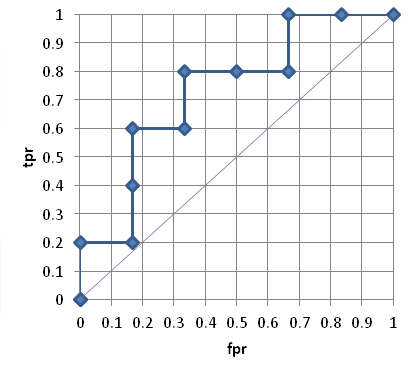
\includegraphics[width=12cm]{ch5_fig2}
  \caption{Financial impact of the different decisions, i.e., False positives, false negatives, 
  true 	positives and true negatives}
	\label{fig:ch5:2}
\end{figure}

In \figurename{ \ref{fig:ch5:2}}, the financial impact of a churn model is shown. Note than we take 
into account the costs and not the profit in each case.
When a customer is predicted to be a churner, an offer is made with the objective of avoiding 
the customer defecting. However, if a customer is actually a churner, he may or not accept the 
offer with a probability $\gamma_i$. If the customer accepts the offer, the financial impact is 
equal to the cost of the offer ($C_{o_i}$) plus the administrative cost of contacting the 
customer ($C_a$). On the other hand, if the customer declines the offer, the cost is the 
expected 	income that the clients would otherwise generate, also called customer lifetime value 
($CLV_i$), 	plus $C_a$. Lastly, if the customer is not actually a churner, he will be happy to 
accept the 	offer and the cost will be $C_{o_i}$ plus $C_a$.
	
In the case that the customer is predicted as non-churner, there are two possible outcomes. 
Either the customer is not a churner, then the cost is zero, or the customer is a churner and the 
cost is $CLV_i$. 


  \begin{table}[b]
	  \centering
	  \footnotesize
     \begin{tabular}{c|c|c}
        \multicolumn{3}{c}{}\\
			\multicolumn{1}{c|}{}  & Actual Positive& Actual Negative \\
			\multicolumn{1}{c|}{} & $y_i=1$& $y_i=0$ \\
			\hline
			Predicted Positive 		& $C_{TP_i}=\gamma_iC_{o_i}$ & 
\multirow{2}{*}{$C_{FP_i}=C_{o_i}+C_a$}\\
%       Predicted Positive    & \multirow{ 
% 2}{*}{$C_{TP_i}=\gamma_iC_{o_i}+(1-\gamma_i)(CLV_i+C_a)$} & 
% \multirow{2}{*}{$C_{FP_i}=C_{o_i}+C_a$}\\
			$c_i=1$ & $+(1-\gamma_i)(CLV_i+C_a)$ &\\
			\hline
			Predicted Negative  	& \multirow{ 2}{*}{$C_{FN_i}=CLV_i$} & \multirow{ 
			2}{*}{$C_{TN_i}=0$} \\
			$c_i=0$ & &\\
			%\hline
		\end{tabular}
		\caption{Proposed churn modeling example-dependent cost matrix}
    \label{tab:ch5:1}
  \end{table}

The different costs are summarized in \tablename{ \ref{tab:ch5:1}}.	Then using the cost 
matrix, and the example-dependent cost-sensitive framework as described in Section 
\ref{sec:3:csmeasures}, an example-dependent cost statistic is calculated as:

\begin{align}
  Cost_i &= y_i(c_i C_{TP_i} + (1-c_i)C_{FN_i})& \nonumber \\
         &  + (1-y_i)(c_i C_{FP_i} + (1-c_i)C_{TN_i})& \nonumber \\
%          &=y_i(c_i (\gamma_iC_{o_i}+(1-\gamma_i)(CLV_i+C_a))& \nonumber \\
%          & + (1-c_i)CLV_i)& \nonumber \\
%          & +  (1-y_i)(c_i (C_{o_i}+C_a) + (1-c_i)(0)) &\nonumber \\
         &= y_i(c_i\left(\gamma_i(C_{o_i}-CLV_i-C_a)-C_{o_i}\right)+CLV_i)&\nonumber \\
         & +c_i(C_{o_i}+C_a),&
	\end{align}
leading to a total cost of:
\begin{equation}
    Cost = \sum_{i=1}^N Cost_i.
\end{equation}
Furthermore, using (\ref{eq:3:savings}), the savings are calculated as:
\begin{equation}
  Savings = \frac{Cost_l - Cost}{Cost_l},
\end{equation} 
In almost all cases the costless class ($Cost_l$) will be the negative class, as typically the 
distribution of a churn dataset is skewed towards the non-churners \citep{Verbeke2012}. Given that 
$Cost_l$ can be expressed as $Cost(f_0)$, or simply $Cost$ with $c_i=0$ $\forall i$:
\begin{equation}
 Cost_l = \sum_{i=1}^{N} y_i CLV_i.
\end{equation}
This is consistent with the notion that if no model is used, the total cost would be the 
sum of the customer lifetime values of the actual churners, which gives the insight 
that the $Savings$ measure consists in comparing the financial impact of the campaign of using a 
classification model against not using a model at all.


\subsubsection{Customer lifetime value}

Lastly, one of the key values to calculate the $Savings$ is the customer lifetime value. Within 
marketing there exists a common misconception between customer profitability and customer lifetime 
value. The two terms are usually used in an interchangeable way, 
creating confusion of what the actual objective of a churn modeling campaign should be. Several 
studies have proposed models providing a unique definition of both terms 
\citep{Neslin2006,Pfeifer2004,Milne1999a,VanRaaij2003}. Customer 
profitability indicates the difference between the income and the cost 
generated by a customer $i$ during a financial period $t$. It is defined as: 
\begin{equation}
	CP_{i,t} = \mu  \cdot s_{i,t},
\end{equation}
where  $s_{i,t}$ refers to the consumption of customer $i$ during time period $t$, and $\mu$ refers 
to the average marginal profit by unit product usage.  

Moreover, we are interested to see what is the expected income that a particular customer will 
generate in the future, in other words, calculating the expected sum of 
discount future earnings \citep{Neslin2006}. Therefore, the $CLV_i$ is defined as:
\begin{equation}
	CLV_i = \sum_{t=1}^T\frac{\mu \cdot s_{i,t}}{(1+r)^t},
\end{equation}
where $r$ is the discount rate, and $T$ the number of time period.
Typically $T$ should be considered large enough since without prior 
knowledge a customer is expected to keep being a customer for the foreseeable future. In practice 
$T$ is set up to be infinity~\citep{Glady2009}. Also, for simplicity, it can be assumed that 
$s_{i,t+1}=s_{i,t}\cdot (1+g)$ $\forall {i,t}$, which means that there is a constant growth $g$ in 
the customer consumption. Given that, the customer lifetime value can be re-written as
\begin{equation}
 CLV_i = \sum_{t=1}^\infty\frac{ (1+g)^t}{(1+r)^t}\cdot \mu\cdot s_{i,1},
\end{equation}
which in the case of $g<r$, this is a geometric series and can be expressed as
\begin{equation}
 CLV_i = \frac{\mu\cdot s_{i,1}}{(r-g)}.
\end{equation}


\subsection{Churn modeling database}
\label{sec:5:1:data}

For our experiments we use a dataset provided by a TV cable provider. 
The dataset consists of active customers during the first semester of 2014. 	
The total dataset contains 9,410 individual registries, each one with 45 attributes, 
including a churn label indicating whenever a customer is a churner.
This label was created internally in the company, and can be regarded as highly accurate. 
In the dataset only 455 customers are churners, leading to a churn ratio of 4.83\%.
	
\subsubsection{Offer acceptance calculation}

In practice companies have a set of offers to make to a customer as part of the retention 
campaign. They vary from discounts to upgrades, among others. In the particular case of a TV cable 
provider, the offers include adding a new set of channels, changing the TV receiver to one with new 
technology (i.e., high definition, video recording, 4K),  or to offer a discount on the monthly 
bill. Unsurprisingly, not all offers apply to all clients. For instance, a customer that already 
has all  the channels can not be offered a new set of channels. Moreover, an offer usually means an 
additional cost to the company and not all offers have the same cost or the same impact in 
reducing churn.

Taking into account the cost and the implication of the offers, the problem can be 
summarized in making each customer the offer that will maximize the acceptance rate and more 
importantly reduce the overall cost. 

\begin{figure}[t!]
  \centering
   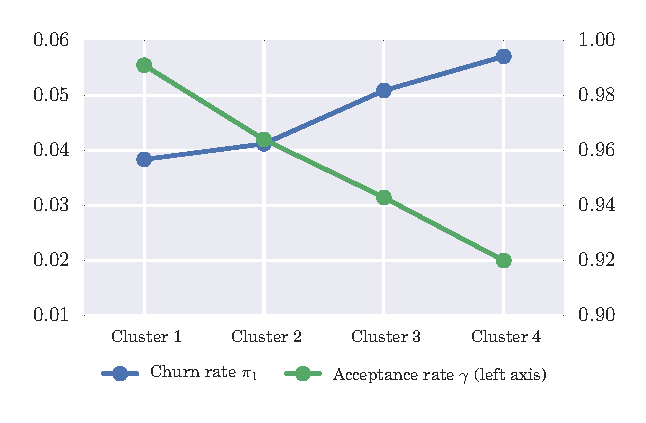
\includegraphics[width=10cm]{ch5_fig3}
  \caption{Acceptance rate ($\gamma$) of the best offer for each customer profile. As expected, 
	the higher the churn rate the lower the acceptance rate, as it is more difficult to make a 
	good offer to a customer which is more likely to defect. }
  \label{fig:ch5:3}
\end{figure}

In order to calculate the acceptance probability $\gamma_i$ a champion-challenger process was made. 
First, the customers were grouped into clusters according to their behavioral and socio-economical 
characteristics. In particular the K-means algorithm was used \citep{Marslan2009}.
Then for a period of two months, randomly selected offers were made to the customers and their 
response was evaluated. Unfortunately, for confidentiality reasons we can not describe the 
different clusters, or the actual offer made to each customer. Nevertheless, in 
\figurename{~\ref{fig:ch5:3}}, the average churn rate and acceptance rate $\gamma_i$ per cluster is 
shown. As expected, the higher the churn rate the lower the acceptance rate, as it is more difficult 
to make a good offer to a customer that is more likely to defect.


\section{Direct marketing}
\label{sec:5:directmarketing}

In direct marketing the objective is to classify those customers who are more likely to have a 
certain response to a marketing campaign \citep{Ngai2009}. We used a direct marketing dataset 
\citep{Moro2011} available on the UCI machine learning repository \citep{UCI2013}. The dataset 
contains 45,000 clients of a Portuguese bank who were contacted by phone between March 2008 and 
October 2010 and received an offer to open a long-term deposit account with attractive interest 
rates.  The dataset contains features such as age, job, marital status, education, average yearly 
balance and current loan status and the label indicating whether or not the client accepted 
the offer.

This problem is example-dependent cost sensitive, since there are different costs of false 
positives and false negatives. Specifically, in direct marketing, false positives have the cost 
of contacting the client, and false negatives have the cost due to the loss of income by failing 
to contact a client that otherwise would have opened a long-term deposit. 
  
\begin{table}[b]
  \centering
  \footnotesize
  \begin{tabular}{c|c|c}
    \multicolumn{1}{c|}{}  & Actual Positive& Actual Negative \\
    \multicolumn{1}{c|}{} & $y_i=1$& $y_i=0$ \\
    \hline
    Predicted Positive    & \multirow{ 2}{*}{$C_{TP_i}=C_a$} & \multirow{ 2}{*}{$C_{FP_i}=C_a$} 
    \\
    $c_i=1$ & &\\
    \hline
    Predicted Negative    & \multirow{ 2}{*}{$C_{FN_i}=Int_i$} & \multirow{ 2}{*}{$C_{TN_i}=0$} 
    \\
    $c_i=0$ & &\\
    %\hline
  \end{tabular}
  \caption{Direct marketing example-dependent cost matrix}
  \label{tab:5:d_mat}
\end{table}

We propose a direct marketing example-dependent cost matrix as shown in \mbox{\tablename{ 
\ref{tab:5:d_mat}}}. Where $C_a$ is the administrative cost of contacting the client, as is credit 
card fraud,  and $Int_i$ is the expected income when a client opens a long-term deposit. This last 
term is defined as the long-term deposit amount times the interest rate spread.
 
In order to estimate $Int_i$, first the long-term deposit amount is assumed to be a 20\% of the 
average yearly balance, and lastly, the interest rate spread is estimated to be 2.463\%,  which 
is the average between 2008 and 2010 of the retail banking sector in Portugal as reported by the 
Portuguese central bank. Given that, the $Int_i$ is equal to $\left( balance * 20\% \right) * 
2.463\%$.


\section{Summary of the datasets}

For each dataset we used a pre-define cost matrix as shown in Section~\ref{sec:5:churn} and 
Section~\ref{sec:5:directmarketing}. Additionally,  for each database, 3 different 
datasets are extracted: training, validation and testing. Each one containing 50\%, 25\% and 25\% 
of the examples, respectively. Afterwards, because classification algorithms suffer when the label 
distribution is skewed towards one of the classes \citep{Hastie2009}, an under-sampling of the 
positive examples is made, in order to have a balanced class distribution. Moreover, we perform the 
cost-proportionate rejection-sampling and cost proportionate over-sampling procedures, that we 
previously described in Section~\ref{sec:3:costsampling}. \tablename{~\ref{tab:5:databases}}, 
summarizes the different datasets. It is important to note that the sampling procedures were only 
applied to the training dataset since the validation and test datasets must reflect the real 
distribution.
\newpage

\begin{table}[ht!]
  \centering
  \footnotesize
  \begin{tabular}{l l c c c } %sum 7.7
    \hline
    \textbf{Database}& \textbf{Set}&  $N$ & $\pi_1$ & Cost (Euros) \\
    \hline
    Churn&Total&9,410&4.83&580,884\\
    Modeling&Training ($t$)&3,758&5.05&244,542\\
    &Under-sampled ($u$) &374&50.80&244,542\\
    &Rejection-sampled ($r$)&428&41.35&431,428\\
    &Over-sampled ($o$) &5,767&31.24&2,350,285\\
    &Validation&2,824&4.77&174,171\\
    &Testing&2,825&4.42&162,171\\
    \hline
    Direct &Total&37,931&12.62&59,507\\
    Marketing&Training ($t$)&15,346&12.55&24,304\\
    &Under-sampled ($u$)&3,806&50.60&24,304\\
    &Rejection-sampled ($r$)&1,644&52.43&20,621\\
    &Over-sampled ($o$)&22,625&40.69&207,978\\
    &Validation&11,354&12.30&16,154\\
    &Testing&11,231&13.04&19,048\\
    \hline
  \end{tabular}
  \caption{Summary of the datasets. Where $N$ is the number of examples and $\pi_1$ is the 
  percentage of positives examples.}
  \label{tab:5:databases}
\end{table}
 
 \makeatletter
\setlength{\@fptop}{0pt}
\makeatother\cleardoublepage

\part{Proposed Cost-Sensitive Classification Methods}

	
\chapter{Bayes minimum risk}
\todo{change notation}

\begin{remark}{Outline}
\todo{outline}
In this chapter, we present the well-known family of \textit{random forests}
methods. In Section~\ref{sec:4:bias-variance}, we first describe the bias-variance
decomposition of the prediction error and then present, in
Section~\ref{sec:4:ensemble}, how aggregating randomized models through
ensembles reduces the prediction error by decreasing the variance term in this
decomposition. In Section~\ref{sec:4:random-forests}, we revisit random forests
and its variants and study how randomness introduced into the decision trees
reduces prediction errors by decorrelating the decision
trees in the ensemble. Properties and features of random forests are then outlined
in Section~\ref{sec:4:features} while their consistency
is finally explored in Section~\ref{sec:4:consistency}.
\end{remark}

\todo{INTRO BMR}

  In this paper two different methods for calibrating probabilities are evaluated and analyzed in 
the context
  of credit card fraud detection, with the objective of finding the model that minimizes the real 
losses due to fraud.
  First, the method proposed \mbox{in \citep{Elkan2001}} to adjust the probabilities based on the 
difference in
  bad rates between the training and testing datasets is used.
  Second, it is compared against the method proposed \mbox{in \citep{Hernandez-Orallo2012}},
  in which calibrated probabilities are extracted after modifying the receiver operating 
characteristic (ROC) curve
  to a convex one using the ROC convex hull methodology.
  
\section{BMR Model}

   We use Bayes minimum risk as a method for cost sensitive credit card fraud detection.
   As defined in \citep{Ghosh2006}, the Bayes minimum risk classifier is a decision model based on
   quantifying tradeoffs between various decisions using probabilities and the costs that accompany 
such decisions.
   In the case of credit card fraud detection, there are two decisions, either predict a 
transaction as fraud $p_f$ or as legitimate $p_l$.
   The risk associated with predicting a transaction as fraud is defined as
   \begin{equation}
    R(p_{f}|x)=L(p_{f}|y_{f})P(p_{f}|x)+L(p_{f}|y_{l})P(p_{l}|x),
    \label{Bayes_min1}
   \end{equation}
   and when the transaction is predicted as legitimate it is
   \begin{equation}
    R(p_{l}|x)=L(p_{l}|y_{l})P(p_{l}|x)+L(p_{l}|y_{f})P(p_{f}|x),
    \label{Bayes_min2}
   \end{equation}
   where %$p_f$ and $p_l$ indicate whether a transaction is predicted as fraud or legitimate, and
   $y_f$ and $y_l$ are the real labels for fraudulent and legitimate transactions respectively. 
$P(p_l|x)$ is the 
   estimated probability of a transaction being legitimate given $x$, similarly 
   $P(p_f|x)$ is the probability of a transaction being fraud given $x$.
   Finally $L(a,b)$ is the loss function when a transaction is predicted as $a$ and the
   real label is $b$.
   Once both risks are calculated, %the decision will be made by choosing the one with the lowest 
cost
   a transaction is classified as fraud if $R(p_{f}|x)\le R(p_{l}|x)$, meaning if the risk 
associated with
   that decision is lower than the risk associated with classifying it as legitimate. % as defined 
in (\ref{Bayes_min3}).
   
   %\noindent 
   Since in the credit card fraud detection case the losses are equal to the cost, first we use 
   the cost matrix with fixed cost for $FN$ as defined in \tablename{ 
\ref{table_measure_cost_hand}}.
   Then a transaction will be classified as fraud if: $C_aP(p_{f}|x)+C_aP(p_{l}|x) \le 
100C_aP(p_{f}|x)$, 
   %the Bayes minimum risk classifier using this cost matrix is defined in (\ref{Bayes_min4}).
   \begin{equation}
    C_aP(p_{f}|x)+C_aP(p_{l}|x) \le 100\cdot C_aP(p_{f}|x),
    \label{Bayes_min4}
   \end{equation}
   and as legitimate otherwise.
  
\section{Calibration of probabilities}

  When using the output of a binary classifier as a basis for decision making,
  there is a need for a probability that not only separates well between 
  positive and negative examples, but that also assesses the real probability of the event 
	\citep{cohen2004}.
  
  In this section two methods for calibrating probabilities are explained.
  First, the method proposed in [6] to adjust the probabilities based on the difference in bad rates
  between the training and testing datasets.
  Then, the method proposed in [8], in which calibrated probabilities are extracted after
  modifying the ROC curve using the ROC convex hull methodology, is described.
  
  \subsection{Brier score and reliability diagrams}
  \todo{Figure of the reliabily diaframs or calibration map}
  
  \subsection{Calibration of probabilities due to a change in base rates.}
  One of the reasons why a probability may not be calibrated is because 
  the algorithm is trained using a dataset with a different base rate than the one on
  the evaluation dataset. 
  This is something common in machine learning since
  using under-sampling or over-sampling is a typical method to solve problems such as
  class imbalance and cost sensitivity \citep{Hulse2007}.
  
  In order to solve this and find probabilities that are calibrated, in \citep{Elkan2001} a formula
  that corrects the probabilities based on the difference of the base rates is proposed.
  The objective is using $p=P(j=1|x)$ which was estimated using a population with base rate 
\mbox{$b=P(j=1)$},
  to find $p'=P'(j=1|x)$ for the real population which has a base rate $b'$.
  A solution for $p'$ is given as follows:
  \begin{equation}
  p'=b'\frac{p-pb}{b-bp+b'p-bb'}.
  \label{cal_prob_br}
  \end{equation}
  Nevertheless, a strong assumption is made by taking: 
  \mbox{$P'(x|j=1)=P(x|j=1)$} and \mbox{$P'(x|j=0)=P(x|j=0)$}, meaning that there
  is no change in the example probability within the positive and negative
  subpopulations density functions.
  
  \subsection{Calibrated probabilities using ROC convex hull.}
  In order to illustrate the ROC convex hull approach proposed in \citep{Hernandez-Orallo2012},
  let us consider the set of probabilities given in \figurename{ \ref{table_example_prob}}.
  Their corresponding  ROC curve of that set of probabilities is shown in \figurename{ 
\ref{ROC_1}}.  It can be seen that this set of probabilities is not calibrated, since at 0.1 there 
is a positive example  followed by 2 negative examples. That inconsistency is represented in the ROC 
curve as a non convex segment  over the curve.
  
  In order to obtain a set of calibrated probabilities, first the ROC curve must be modified in 
order to be convex.
  The way to do that, is to find the convex \mbox{hull \citep{Hernandez-Orallo2012}}, 
  in order to obtain the minimal convex set containing the different points of the ROC curve.
  In \figurename{ \ref{ROC_2}}, the convex hull algorithm is applied to the previously evaluated 
ROC curve.
  It is shown that the new curve is convex, and includes all the points of the previous ROC curve.
  
  Now that there is a new convex ROC curve or ROCCH, the calibrated probabilities can be extracted 
as shown
  in  \figurename{ \ref{cal_prob}}. The procedure to extract the new probabilities is to first group 
the
  probabilities according to the points in the ROCCH curve, and then make the calibrated
  probabilities be the slope of the ROCCH for each group.
  
\begin{figure}[!t]
\hskip 0.5cm
\hbox{
  \vtop{
    \hbox{
      \subfloat[Set of probabilities and their respective class label]{
	\begin{tabular}{cc}
	\hline
	Probability & Label\\
	\hline
	0.0&	0\\
	0.1&	1\\
	0.2&	0\\
	0.3&	0\\
	0.4&	1\\
	0.5&	0\\
	0.6&	1\\
	0.7&	1\\
	0.8&	0\\
	0.9&	1\\
	1.0&	1\\
	\hline
	\end{tabular}\label{table_example_prob}
      }
    }
  }\hskip 0.5cm
  \vtop{\vskip -2.5cm
    \subfloat[ROC curve of the set of probabilities]{
      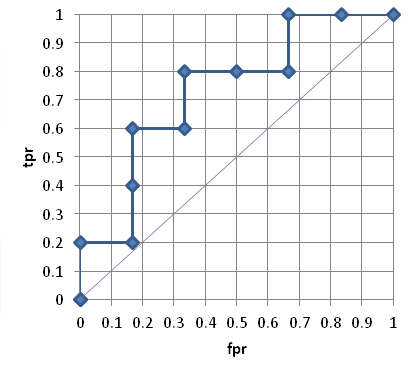
\includegraphics[scale=0.5]{ch6_fig2}\label{ROC_1}
    }%
  }%
}
\vskip 1.5cm

\hbox{ 
  \vtop{ \vskip 0.5cm
    \hbox{
      \subfloat[Convex hull of the ROC curve]{
	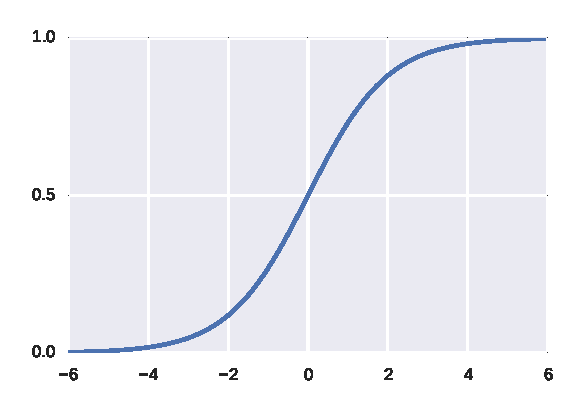
\includegraphics[scale=0.5]{ch6_fig1}\label{ROC_2}
      }
    }
  }\hskip 1cm
  \vtop{ \vskip -1cm
    \subfloat[Calibrated probabilities]{
	\begin{tabular}{cc}
	\hline
	Prob & Cal Prob\\
	\hline
	0.0&	0\\
	0.1&	0.333\\
	0.2&	0.333\\
	0.3&	0.333\\
	0.4&	0.5\\
	0.5&	0.5\\
	0.6&	0.666\\
	0.7&	0.666\\
	0.8&	0.666\\
	0.9&	1\\
	1.0&	1\\
	\hline
	\end{tabular}\label{cal_prob} 
    }
  }
}
\caption{Estimation of calibrated probabilities using the ROC convex hull 
\citep{Hernandez-Orallo2012}.}\label{fig1}

\end{figure}
   
\section{Experiments}
\cleardoublepage
	\chapter{Cost-sensitive decision trees}\label{ch:7}

\begin{remark}{Outline}
In this chapter, we introduce the decision tree algorithm in Section \ref{sec:7:dt}. Then, in 
Section \ref{sec:7:csdt}, we described our previously proposed cost-sensitive decision tree. For 
this, we first shown the new cost-sensitive impurity measure, that introduces the diferent costs 
when evaluating the performance of a split. Then, we introduce a new cost-sensitive pruning 
criteria. Finally, in Section \ref{sec:7:experiments}, we compare the results of the proposed 
algorithm, against state-of-the-art methods, using the five real-world cost-sensitive databases.
\end{remark}

\section{Decision trees}
\label{sec:7:dt}

Decision trees are one of the most widely used machine learning algorithms \citep{Lior2008}. 
The technique is considered to be white box, in the sense that is easy to interpret, and has a 
very low computational cost, while maintaining a good performance as compared with more complex 
techniques \citep{Hastie2009}. There are two types of decision tree depending on the objective of 
the model. They work either for classification or regression. In this section we focus on
binary classification decision tree.

\subsection{Construction of classification trees}

Classification trees is one of the most common types of decision tree, in which the objective 
is to find the $Tree$ that best discriminates between classes. In general the decision tree 
represents a set of splitting rules organized in levels in a flowchart structure.

\subsubsection{Splitting criteria}

In the $Tree$, each rule is shown as a node, and it is represented as $(\mathbf{x}^j,l^j)$, meaning 
that the 
set $\mathcal{S}$ is split in two sets $\mathcal{S}^l$ and $\mathcal{S}^r$ according to 
$\mathbf{x}^j$ and $l^j$:
\begin{equation}
  \mathcal{S}^l = \{\mathbf{x}^a_i \vert \mathbf{x}^a_i \in \mathcal{S} \wedge x^j_i \le l^j \},
\end{equation}
and
\begin{equation}
  \mathcal{S}^r = \{\mathbf{x}^a_i \vert \mathbf{x}^a_i \in \mathcal{S} \wedge x^j_i > l^j \},
\end{equation}
where $\mathbf{x}^j$ is the $j^{th}$ feature represented in the vector 
$\mathbf{x}^j=[x_1^j,x_2^j,...,x_N^j]$, and $l^j$ is a value such that $min(\mathbf{x}^j) \le l^j < 
max(\mathbf{x}^j)$. Moreover, $\mathcal{S} = \mathcal{S}^l \cup \mathcal{S}^r$.

After the training set have been split, the percentage of positives in the different sets is 
calculated. First, the number of positives in each set is estimated by
\begin{equation}
 \mathcal{S}_1 = \{\mathbf{x}^a_i \vert \mathbf{x}_i^a \in \mathcal{S} \wedge y_i =1 \},
\end{equation}
then the percentage of positives is calculates as
\begin{equation}
 \pi_1=\vert \mathcal{S}_1 \vert / \vert \mathcal{S} \vert.
\end{equation}

Then, the impurity of each leaf is calculated using either a misclassification error, 
entropy or Gini measures:
\begin{itemize}
 \item  Misclassification
 \begin{equation}
 I_m(\pi_1)=1-max(\pi_1,1-\pi_1)
 \end{equation}
 
 \item Entropy
 \begin{equation}
 I_e(\pi_1)=-\pi_1\log \pi_1 -(1-\pi_1) \log (1-\pi_1)
 \end{equation}
 
 \item Gini
 \begin{equation}
 I_g(\pi_1)=2\pi_1(1-\pi_1)
 \end{equation}
\end{itemize}

In \figurename{ \ref{fig:7:impurity}}, the three measures are shown. All measures are similar, with 
the exception that the gini index and the cross-entropy are differentiable, which makes them
more suitable for numerical optimization.
\begin{figure}[t!]
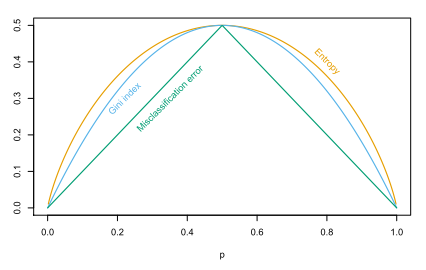
\includegraphics[scale=0.85]{ch7_fig1}
\caption{Impurity measures for a binary classification, as a function of the proportion of
positive examples in the set (Cross-entropy is scaled) \citep{Hastie2009}.}
\label{fig:7:impurity}
\end{figure} 

Finally the gain of the splitting criteria using the rule $(\mathbf{x}^j,l^j)$ is calculated as the 
impurity of $\mathcal{S}$ minus the weighted impurity of each leaf:
\begin{equation}\label{eq:7:gain}
  Gain(\mathbf{x}^j,l^j)=I(\pi_1)-\frac{\vert \mathcal{S}^l \vert}{\vert \mathcal{S} 
\vert}I(\pi^l_1)  -\frac{\vert \mathcal{S}^r \vert}{\vert \mathcal{S} \vert}I(\pi^r_1),
\end{equation} 
where $I(\pi_1)$ can be either of the impurity measures $I_e(\pi_1)$ or $I_g(\pi_1)$.

Subsequently, the gain of all possible splitting rules is calculated. The rule with maximal 
gain is selected
\begin{equation}
  (best_x, best_l) = \argmax_{(\mathbf{x}^j,l^j)}Gain(\mathbf{x}^j,l^j),
\end{equation}
and the set $\mathcal{S}$ is split into $\mathcal{S}^l$ and $\mathcal{S}^r$ according to that rule. 


\subsubsection{Tree growing}
In order to grow a tree typical algorithms use a top-down induction using a greedy search in each
iteration \citep{Rokach2010}. In each iteration, the algorithms evaluates all possible splitting 
rules and pick the one that maximizes the splitting criteria. After the selection of a splitting 
rule, each leaf is further selected and it is subdivides into smaller leafs, until one of the 
stopping criteria is meet. In Algorithm \ref{alg:7:tree_grow}, the pseudocode of the tree 
growing procedure is presented.

\begin{algorithm}\label{alg:7:tree_grow}
Pseudocode of the tree growing procedure.
\textnormal{
\begin{algorithmic}[1]
\Function{TreeGrow}{$\mathcal{S}$}
    \State $Tree = Empty$
    \If{\Call{Stopping}{$Tree, \mathcal{S}$}}
      \State \Return $Tree$
     \EndIf
    \State \# For all features
    \For{$j=1 \  to \ k$}
      \State \# For all possible thresholds
      \For{$m=1 \ to N_k$}
        \State $Gains(j,m) = $ \Call{Gain}{$\mathbf{x}^j,l^j_m, \mathcal{S}$}
      \EndFor
    \EndFor
    \State \# Select the threshold with the highest gain
    \State $(j^*, l^*) = argmax_{(j,m)}Gains$
    \State \# Split the set using the best rule
    \State $\mathcal{S}^l = \{\mathbf{x}^a_i \vert \mathbf{x}_i^a \in \mathcal{S} 
            \wedge \mathbf{x}_i^{j^*} \le l^* \}$
    \State $\mathcal{S}^r = \{\mathbf{x}^a_i \vert \mathbf{x}_i^a \in \mathcal{S} 
            \wedge \mathbf{x}_i^{j^*} > l^* \}$
    \State \# Recursively continue growing tree
    \State \Call{TreeGrow}{$\mathcal{S}^l$}
    \State \Call{TreeGrow}{$\mathcal{S}^r$}
    \State \# Return the tree
    \State \Return $Tree$
\EndFunction
\end{algorithmic}
}
\end{algorithm}

  
\subsubsection{Stopping criteria}
As the growing phase of the algorithm continue, at each iteration the stopping criteria are 
evaluated \citep{Rokach2010}. The most common stopping criteria are:
 \begin{itemize}
   \item All examples in the set belong to the same class. Meaning that either $\pi_1=1$ or 
    $\pi_1=0$.

  \item The maximum number of iterations have been reached.
  
  \item The number of examples in $\mathcal{S}$ are less than the minimum number of examples 
defined for a split.
  
  \item The number of examples in $\mathcal{S}^l$ or $\mathcal{S}^r$ are less than the minimum 
number of examples defined for a leaf.
  
  \item The best splitting rule has a Gain lower than a defined threshold.
\end{itemize}


\subsubsection{Pruning techniques}
After a decision tree has been fully grown, there is the big chance that  the algorithm generates a 
large tree that is probably over fitting the  training data. In order to solve this in 
\citep{Breiman1984a} originally suggest the use of pruning techniques after the tree growing phase.
The overall objective of pruning is to eliminate branches that are not contributing
to the generalization accuracy of the \mbox{tree \citep{Rokach2010}.}
 
In general pruning techniques start from a fully grown tree, and recursively check if by eliminating 
a $Branch$ there is an $Improvement$ in the error rate $\epsilon$ of the $Tree$.  There are two main 
methods to calculate the $Improvement$ of the error rate $\epsilon$ of the $Tree$, cost-complexity 
and  error based pruning:
  
\begin{itemize}
\item Cost-complexity pruning:
  
Initially proposed by Breiman  \citep{Breiman1984a}, this method evaluate iterative if the removal 
of a $Branch$ improve the error rate $\epsilon$ of a $Tree$, weighted by the difference of the 
number of leafs trees.
\begin{equation}\label{eq:7:pruning}
PC_{cc} = \frac{\epsilon(EB(Tree,branch),S)-\epsilon(Tree,\mathcal{S}) }
{\vert Tree\vert-\vert EB(Tree,branch)\vert}
\end{equation} 
where $\epsilon(Tree,\mathcal{S})$ calculate the error rate of the $Tree$ in set $\mathcal{S}$ and 
$EB(Tree,branch)$ is an auxiliary function that removes $branch$ from $Tree$ and return a new 
$Tree$. At each iteration, the current $Tree$ is compared against all possible $Branches$.
    
\item Error based pruning:
  
This method proposed by Quinlan  \citep{Quinlan1992} is more pessimistic and instead of  using the 
error rate $\epsilon$ calculate the upper bound of the confidence interval   of the error 
$\epsilon_{UB}$ calculated assuming a normal distribution with a defined significance level 
$Z_\alpha$.
\begin{equation}
PC_{eb} = \frac{\epsilon_{UB}(EB(Tree,branch),\mathcal{S})-\epsilon_{UB}(Tree,\mathcal{S}) }
    {\vert Tree\vert-\vert EB(Tree,branch)\vert}
\end{equation} 
where 
\begin{align}
    \epsilon_{UB}(Tree,&\mathcal{S})= \epsilon(Tree,\mathcal{S}) & \nonumber \\
    &+Z_\alpha \sqrt{  
\frac{\epsilon(Tree,\mathcal{S})(1-\epsilon(Tree,\mathcal{S}))}{\vert \mathcal{S} \vert}} &
\end{align}   
Moreover, as a difference from cost-complexity pruning, in the error based method, at each 
iteration not all the branches are compared, but only the ones on the same level. Meaning leafs 
are only compared against other leafs that are in the same level of iterations when the $Tree$ 
was constructed. This allows for much faster pruning procedure.
\end{itemize}

In Algorithm~\ref{alg:7:tree_pruning}, the general method of pruning is shown. The pruning 
procedure consists in evaluating the $Improvement$ of eliminating all possible branches in a $Tree$, 
and then eliminate the one with the higher $Improvement$ and repeat the process until a stopping 
criteria is meet.

\begin{algorithm}\label{alg:7:tree_pruning}
Pseudocode of the tree pruning procedure.
\textnormal{
\begin{algorithmic}[1]
\Function{TreePruning}{$\mathcal{S}, Tree$}
    \State \# For all branches
    \For{$branch \  in \ Tree.branches$}
      \State \# Evaluate the pruning criteria
      \State $Improvements(branch) = $ \Call{PC}{$\mathcal{S}, Tree, branch$}
    \EndFor
    \State \# Select the branch to prune
    \State $branch^* = argmax_{branch} Improvements$
    \State \# Prune selected branch
    \State $Tree = $ \Call{EB}{$TreeTree,branch^*$}
    \State \# Recursively continue pruning the tree
    \State \Call{TreePruning}{$\mathcal{S}, Tree$}
    \State \Return $Tree$
\EndFunction
\end{algorithmic}
}
\end{algorithm}

 
\subsubsection{Categorical features}
When using continuous features the splitting is done by testing all possible thresholds on the 
database and  selecting the one that maximizes the desired measure. Nevertheless, this is not 
straight forward when using a  categorical feature, since testing all possible ways of binning the 
feature becomes prohibitively time  consuming the feature has many categories. Instead, a common 
method for doing this is to calculate $\pi_1$ of each category, then sort it, and applied the 
method as a continuous feature \citep{Marslan2009}.



\subsection{Decision tree algorithms}
% \begin{remark}{Decision tree algorithms}
Two main branches of decision trees has being studied in the last years. The main difference is 
the  impurity measure used when splitting. First the CART algorithm that is based in the Gini 
index, and  later the ID3 and C4.5 which uses the entropy measure.

\begin{itemize}
 \item 
  CART or classification and regression trees was introduced by Brieman et al. in 1984 
\citep{Breiman1984a}. It is based on using the Gini index as the impurity measure and the tree is 
grow until all examples in  each leaf belong to the same class. Afterwards, the tree is pruned using 
the cost-complexity  method \citep{Rokach2010,Marslan2009}.
  
\item ID3
  algorithm uses entropy as the impurity measure. The growing of the tree stop when all 
examples belong  of each leaf belongs to the same class. In ID3 no pruning is applied 
\citep{Quinlan1992}.
  
\item C4.5
  the extension of ID3 both proposed by Quinlan \citep{Quinlan1992}.  Both are similar 
regarding the measure used, but C4.5 define the stopping criteria during the growth process
  to be when the number of examples in a set is less than a threshold. Moreover, after the tree is 
created  a error based pruning is applied \citep{Rokach2010}.
\end{itemize} 
% \end{remark}


\section{Example-Dependent Cost-sensitive Decision Trees}
\label{sec:7:csdt}

Standard decision tree algorithms focus on inducing trees that maximize accuracy. However this is 
	not optimal when the misclassification costs are unequal \citep{Elkan2001}. This has led to many 
	studies that develop algorithms that aim to introduce the cost-sensitivity into the algorithms 
	\citep{Lomax2013}. These studies have focused on introducing the class-dependent costs  
	\citep{Draper1994,Ting2002,Ling2004,Li2005,Kretowski2006,Vadera2010}, which is not optimal for 
	some applications. For example in credit card fraud detection, it is true that false positives 
	have a different cost than false negatives, nevertheless, false negatives may vary significantly, 
	which makes class-dependent cost-sensitive methods not suitable for this problem.
      
  In this section, we first propose a new method to introduce the costs into the decision tree 
	induction stage, by creating new-cost based impurity measures. Afterwards, we propose a new 
	pruning method based on minimizing the cost as pruning criteria.

	\subsection{Cost-sensitive impurity measures}

		Standard impurity measures such as misclassification, entropy or Gini, take into account the 
		distribution of classes of each leaf to evaluate the predictive power of a splitting rule,
		leading to an impurity measure that is based on minimizing the misclassification rate. However, 
		as has been previously shown \citep{CorreaBahnsen2013}, minimizing misclassification does not 
		lead to the same results than minimizing cost. Instead, we are interested in measuring how good 
		is a splitting rule in terms of cost not only accuracy. For doing that, we propose a new 
		example-dependent cost based impurity measure that takes into account the cost matrix of each 
		example.

		We define a new cost-based impurity measure taking into account the costs when all the examples
		in a leaf are classified both as negative using $f_0$ and positive using $f_1$
		\begin{equation}\label{eq:cost_impurity}
			I_c(\mathcal{S}) = \min \bigg\{ Cost(f_0(\mathcal{S})), Cost(f_1(\mathcal{S})) \bigg\}.
		\end{equation}
		The objective of this measure is to evaluate the lowest expected cost of a splitting rule.
		Following the same logic, the classification of each set is calculated as the prediction that 
		leads to the lowest cost
	  \begin{equation}\label{eq_pred}
	    f(\mathcal{S}) = 
	    \begin{cases}
	      \phantom{-}0 \phantom{-} \mbox{if} \phantom{-} Cost(f_0(\mathcal{S})) \le 
        Cost(f_1(\mathcal{S}))\\
	      \phantom{-}1 \phantom{-}\mbox{otherwise}
	    \end{cases}
	  \end{equation}

		Finally, using the cost-based impurity, the splitting criteria cost based gain of using the 
		splitting rule $(\mathbf{x}^j,l^j)$ is calculated with (\ref{eq:7:gain}). 

	\subsection{Cost-sensitive pruning}
 
		Most of the literature in class-dependent cost-sensitive decision tree focuses on using the 
		misclassification costs during the construction of the algorithms \citep{Lomax2013}. Only few 
		algorithms such as AUCSplit \citep{Ferri2002} have \mbox{included} the costs both during and 
		after the construction of the tree. However, this approach only used the class-dependent costs, 
		and not the example-dependent costs.
 
		We propose a new example-dependent cost-based impurity measure, by replacing the error rate 
		$\epsilon$ in (\ref{eq:7:pruning}) with the cost of using the $Tree$ on $\mathcal{S}$ i.e. by 
    replacing with 	$Cost(f(\mathcal{S}))$.
		\begin{equation}\label{eq:cost_pruning}
			PC_{c} = \frac{ Cost(f(\mathcal{S})) - Cost(f^*(\mathcal{S})) }
		  {\vert Tree\vert-\vert EB(Tree,node)\vert} ,
		\end{equation}
		where $f^*$ is the classifier of the tree without the selected node $EB(Tree,node)$.
 
		Using the new pruning criteria, nodes of the tree that do not contribute to the minimization of 
		the cost will be pruned, regardless of the impact of those nodes on the accuracy of the
		algorithm. This follows the same logic as in the proposed cost-based impurity measure, since 
		minimizing the misclassification is different than minimizing the cost, and in several 
		real-world applications the objectives align with the cost not with the misclassification error.
		
\section{Experiments}
\label{sec:7:experiments}

\cleardoublepage
	\chapter{Ensembles of cost-sensitive decision trees}

\begin{remark}{Outline}
In this chapter, we introduce the framework of ensembles of example-dependent cost-sensitive 
decision-trees, by training example-dependent cost-sensitive decision trees using four different 
random inducer methods and then blending them using three different combination approaches.
First, in Section \ref{sec:8:ensemble}, we give the background behind ensemble learning. Then, in 
Section \ref{sec:8:ecsdt}, we present our previously proposed ensembles of cost-sensitive 
decision-trees framework. Moreover, in Section \ref{sec:8:theoretical}, we prove theoretically that 
combining individual cost-sensitive classifiers achives better  results in the sense of higher 
financial savings. Afterwards, in Section \ref{sec:8:experiments}, we compare the results of the 
proposed algorithm, against state-of-the-art methods, using the five real-world cost-sensitive 
databases. Finally, in Section \ref{sec:8:experiments_all}, we compare the results of the different 
algorithms presented in this Thesis, using the different databases.
\end{remark}


\section{Ensemble methods}
\label{sec:8:ensemble}

  Ensemble learning is a widely studied topic in the machine learning community. The main
  idea behind the ensemble methodology is to combine several individual base classifiers in
  order to have a classifier that outperforms each of them \citep{Rokach2009}. Nowadays, 
  ensemble methods are  one of the most popular and well studied machine learning techniques 
  \citep{Zhou2012}, and it can be noted that since 2009 all the first-place and 
  second-place winners of the KDD-Cup competition\footnote{https\://www.sigkdd.org/kddcup/} used 
  ensemble methods. The core principle in ensemble learning, is to induce random perturbations into 
  the learning procedure in order to produce several different base classifiers from a single 
  training set, then combining the base classifiers in order to make the final prediction.
  In order to induce the random permutations and therefore create the different base classifiers, 
  several methods have been proposed, in particular: bagging \citep{Breiman1996}, 
  pasting~\citep{Breiman1999}, random forests \citep{Breiman2001} and random patches 
  \citep{Louppe2012}. Finally, after  the base   classifiers are trained, they are typically 
  combined using either   majority voting,  weighted  voting    or  stacking~\citep{Zhou2012}.

As shown in \figurename{~\ref{fig:8:1}, there are three main reasons regarding why ensemble 
methods perform better than single models: statistical, computational and representational 
\citep{Dietterich2000a}. First, from a statistical point of view, when the learning set is too 
small, an algorithm can find several good models withing the search space, that arise to the same 
performance on the training set $\mathcal{S}$. Nevertheless, without a validation set, there is 
the risk of choosing the wrong model. The second reason is computational; in general, algorithms 
rely on some local search optimization and may get stuck in a local optima. Then, an ensemble may 
solve this by focusing different algorithms to different spaces across the training set. The last 
reason is representational. In most cases, for a learning set of finite size, the  true function 
$f$ cannot be represented by any of the candidate models. By combining several  models in an 
ensemble, it may be possible to obtain a model with a larger coverage across the  space of 
representable functions.
  
\begin{figure}[t!]
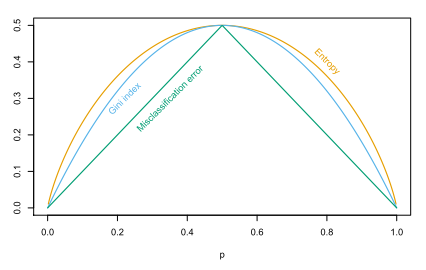
\includegraphics[scale=.5]{ch8_fig1}
\caption{Main reasons regarding why ensemble methods perform better than 
  single models: statistical, computational and representational \citep{Dietterich2000a}.}
\label{fig:8:1}
\end{figure} 
  
  The most typical form of an ensemble is made by combining $T$ different base classifiers.
  Each  base classifier $M(\mathcal{S}_j)$ is trained by applying algorithm $M$ to a random subset 
  $\mathcal{S}_j$ of the training set $\mathcal{S}$.  %  $\mathcal{S_j} = RI(\mathcal{S})$
  For simplicity we define $M_j \equiv  M(\mathcal{S}_j)$ for $j=1,\dots,T$, and 
  $\mathcal{M}=\{M_j\}_{j=1}^{T}$ a set of base classifiers.
  Then, these models are combined using majority voting to create the ensemble $H$ as follows
  \begin{align}\label{eqn:majority-vote}
    f_{mv}(\mathcal{S},\mathcal{M}) = \argmax_{c \in \{0,1\}} \sum_{j=1}^T 
    \mathbf{1}_c(M_j(\mathcal{S})).
  \end{align}

  \newpage
  \begin{remark}{Theoretical performance of an ensemble}
%   Moreover, i
  If we assume that each one of the $T$ base classifiers have a probability $\rho$ of 
  being correct, the probability of an ensemble making the correct decision, denoted by $P_c$,
  can be calculated using the binomial \mbox{distribution \citep{Hansen1990}}
  \begin{equation}\label{eq:prob}
    P_c = \sum_{j>T/2}^{T} {{T}\choose{j}} \rho^j(1-\rho)^{T-j}.
  \end{equation}
  Furthermore, as shown in \citep{Lam1997}, if $T\ge3$ then:
  \begin{itemize}
    \item If $\rho>0.5$, then $ \lim_{T \to  \infty} P_c=1 $
    \item If $\rho<0.5$, then $ \lim_{T \to  \infty} P_c=0 $
    \item If $\rho=0.5$, then $P_c=0.5$ for any $T$.
  \end{itemize}
  Leading to the conclusion that $P_c\ge \rho$ if $\rho \ge 0.5$ for any $T$.
  \end{remark}
  
\subsection{Cost-sensitive ensembles}

  In the context of cost-sensitive classification, some authors have proposed methods for using 
  ensemble techniques. In \citep{Masnadi-shirazi2011}, the authors proposed a framework for 
  cost-sensitive boosting that is expected to minimized the losses by using optimal cost-sensitive 
  decision rules. In \citep{Street2008}, a bagging algorithm with adaptive costs was proposed. In 
  his doctoral thesis, Nesbitt \citep{Nesbitt2010}, proposed a method for cost-sensitive 
  tree-stacking. In this method different decision trees are learned, and then combined in a way 
  that a cost function is minimized. Lastly in \citep{Lomax2013}, a survey of application of 
  cost-sensitive learning with decision trees is shown, in particular including other methods that 
  create cost-sensitive ensembles. However, in all the previously presented method, the 
  misclassification costs only dependent on the class, therefore, assuming a constant cost across 
  examples. Given that, these methods are not  well suited for example-dependent cost-sensitive 
  problems. 

      
\section{Ensembles of cost-sensitive decision trees}
\label{sec:8:ecsdt}

In this section we shown our previously proposed framework of ensembles of  example-dependent 
cost-sensitive  decision-trees \citep{CorreaBahnsen2015b}, by training example-dependent 
cost-sensitive decision trees using four different  random inducer methods and then blending them 
using three different combination approaches. Moreover, we propose two new cost-sensitive 
combination approaches, cost-sensitive weighted  voting and cost-sensitive stacking. The latter 
being an extension of our previously proposed cost-sensitive logistic regression 
\citep{CorreaBahnsen2014b}. 

The remainder of the section is organized as follows: First, we introduce the example-dependent 
cost-sensitive decision tree. Then we present the different random inducers and combination 
methods. Finally, we define our proposed algorithms.
  
 
\section{Theoretical analysis of the ECSDT}
\label{sec:8:theoretical}

    
\section{Experiments}
\label{sec:8:experiments}

\section{Overall experiments}
\label{sec:8:experiments_all}\cleardoublepage

		
	\chapter{Ensembles of cost-sensitive decision trees}
		\section{Ensemble methods}
			\section{Random inducers}
				\subsection{Bagging}
				\subsection{Pasting}
				\subsection{Random forest}
				\subsection{Random patches}
			\section{Combination methods}
				\subsection{Majority voting}
				\subsection{Weighted voting}
				\subsection{Staking}
		\section{Cost-sensitive combination methods}
			\subsection{Cost-sensitive weighted voting}
			\subsection{Cost-section stacking}
		\section{ECSDT}
		\section{Theoretical analysis of the ECSDT}
		\section{Experiments}
			
 
\addtocontents{toc}{\protect\vspace*{\baselineskip}\protect}
\cleardoublepage
\makeatletter
\def\toclevel@chapter{-1}
\makeatother
\chapter{Conclusions}

% % Back pages ==================================================================
\appendix
\cleardoublepage
\part{Appendix}
	\chapter{Costcla - Python package}
		\section{Introduction}
			\subsection{PyEA}
		\section{API}
		\section{Examples}

% Notations ====================================================================

\chapter{Notations}
\todo{take notations from the ECSDT paper}
	
\begin{tabularx}{\textwidth}{ l X }
$\cal S$ 		& Set of examples 		\dotfill \pageref{ntn:ch2:1} \\ 
$\mathcal{S}_{train}$ 	& Training set	 		\dotfill \pageref{ntn:ch2:1} \\
$\mathcal{S}_{test}$ 	& Testing set	 		\dotfill \pageref{ntn:ch2:1} \\
$\mathbf{y}$ 		& Class labels 			\dotfill \pageref{ntn:ch2:1} \\  
$\mathbf{x}_i$ 		& Feature vector of example $i$ \dotfill \pageref{ntn:ch2:1} \\
$k$ 			& Number of features 		\dotfill \pageref{ntn:ch2:1} \\
$N $ 			& Number of examples 		\dotfill \pageref{ntn:ch2:1} \\
$y_i$ 			& Class label of example $i$ 	\dotfill \pageref{ntn:ch2:1} \\
$f(\mathcal{S})$ 	& A classification algorithm 	\dotfill \pageref{ntn:ch2:1} \\
$\mathbf{x}$ 		& Predicted class labels 	\dotfill \pageref{ntn:ch2:1} \\  
$c_i$ 			& Predicted class for example $i$  \dotfill \pageref{ntn:ch2:1} \\
\end{tabularx}
\cleardoublepage
%********************************************************************
% Bibliography
%*******************************************************
% work-around to have small caps also here in the headline
\manualmark
\markboth{\spacedlowsmallcaps{\bibname}}{\spacedlowsmallcaps{\bibname}} % work-around to have small
%\phantomsection 
\refstepcounter{dummy}
\addtocontents{toc}{\protect\vspace{\beforebibskip}} % to have the bib a bit from the rest in the 

\addcontentsline{toc}{chapter}{\tocEntry{\bibname}}
\bibliographystyle{myabbrvnat}
\label{app:bibliography} 
\bibliography{bibliography}
\cleardoublepage
\end{document}
